\documentclass{classes/fiboThesis}

\begin{document}

\title{Structure Design and Platform Development of Universal Template\break for Humanoid Algorithm Interface (UTHAI)}
\titleTH{การออกแบบโครงสร้างและพัฒนาระบบพื้นฐานสำหรับหุ่นยนต์ฮิวมานอยด์\break เพื่อการศึกษาและวิจัย}

\author{นายจิรัฏฐ์ ศรีรัตนอาภรณ์}
\authorTwo{นายเจษฎากร ทาไชยวงค์}
\authorThree{นายวุฒิภัทร โชคอนันตทรัพย์}

\majoradvisor{นายธนัชชา ชูพจน์เจริญ}
\coadvisor{รศ.ดร.ชิต เหล่าวัฒนา}
\committeeOne{ดร.อาบทิพย์ ธีรวงศ์กิจ}
\committeeTwo{ดร.ปิติวุฒญ์ ธีรกิตติกุล}
\committeeThree{ดร.สุภชัย วงศ์บุณย์ยง}

\academicyearTH{2560}

\maketitle
\frontmatter
\maketitleinner
\makeapproval
% ************************** Thesis Abstract **********************************
\begin{abstract}
    งานวิทยานิพนธ์นี้เป็นงานที่เกี่ยวกับการออกแบบและจัดทำแพลตฟอร์มหุ่นยนต์ฮิวมานอยด์ด้วยเครื่องพิมพ์สามมิติ
จุดประสงค์คือเพื่อ
\end{abstract}
% ************************** Thesis Acknowledgements **************************
% \majoradvisor{นายธนัชชา ชูพจน์เจริญ}
% \coadvisor{รศ.ดร.ชิต เหล่าวัฒนา}
% \committeeOne{ดร.อาบทิพย์ ธีรวงศ์กิจ}
% \committeeTwo{ดร.ปิติวุฒญ์ ธีรกิตติกุล}
% \committeeThree{ดร.สุภชัย วงศ์บุณย์ยง}
\begin{acknowledgements}
ขอขอบพระคุณอาจารย์ ธนัชชา ชูพจน์เจริญ อาจารย์ที่ปรึกษาวิทยานิพนธ์หลัก
ที่ได้สละเวลามาให้คำปรึกษา ชี้แนะแนวทาง ให้ความรู้ในด้านต่างๆ ที่จำเป็นต่องานวิจัย รวมถึงการให้การสนับสนุนในเรื่องอุปกรณ์ในการทำวิจัย
ตลอดจนช่วยตรวจและแก้ไขวิทยานิพนธ์ให้เป็นไปอย่างสมบูรณ์

ขอขอบพระคุณรองศาสตราจารย์ ดร.ชิต เหล่าวัฒนา อาจารย์ที่ปรึกษาวิทยานิพนธ์ร่วม
ที่ได้ชี้แนะแนวทาง ให้คำแนะนำ และให้เกียรติเข้าร่วมการสอบวิทยานิพนธ์

ขอขอบพระคุณอาจารย์ ดร.ถวิดา มณีวรรณ และนายวิษณุ จูธารี ที่ได้ให้คำแนะนำในการแก้ไขปัญหาด้านต่างๆ
ที่เกิดขึ้นระหว่างการทำการวิจัย และได้ให้การสนับสนุนอุปกรณ์สำคัญที่ใช้ในการทำวิจัย

ขอขอบพระคุณอาจารย์ อาบทิพย์ ธีรวงศ์กิจ ที่กรุณาให้เกียรติเป็นประธานกรรมการสอบวิทยานิพนธ์
ให้คำแนะนำที่เป็นประโยชน์ต่อการจัดทำวิทยานิพนธ์ให้ดำเนินไปอย่างสมบูรณ์

ขอขอบพระคุณอาจารย์ ดร.ปิติวุฒญ์ ธีรกิตติกุล ที่กรุณาให้เกียรติเป็นกรรมการสอบวิทยานิพนธ์ 
ให้คำแนะนำที่เป็นประโยชน์ต่อการวิจัย และการแก้ไขปรับปรุงงานวิจัย ตลอดจนตรวจแก้วิทยานิพนธ์ให้ดำเนินไปอย่างสมบูรณ์

ขอขอบพระคุณอาจารย์ ดร.สุภชัย วงศ์บุณย์ยง ที่กรุณาให้เกียรติเป็นกรรมการสอบวิทยานิพนธ์ 
ให้คำแนะนำที่เป็นประโยชน์ต่อการวิจัย และการแก้ไขปรับปรุงงานวิจัย ตลอดจนตรวจแก้วิทยานิพนธ์ให้ดำเนินไปอย่างสมบูรณ์

ขอขอบพระคุณคณาจารย์ และบุคลากรในสถาบันวิทยาการหุ่นยนต์ภาคสนามทุกท่าน
ที่ได้ให้คำปรึกษาและช่วยเหลือด้านสถานที่พร้อมทั้งสิ่งอำนวยความสะดวกต่างๆ ในระหว่างการทำวิทยานิพนธ์

ขอขอบคุณนักศึกษาปริญญาตรี สถาบันวิทยาการหุ่นยนต์ภาคสนามทุกท่าน
ที่ได้ให้คำแนะนำ ถามไถ่ และเป็นกำลังใจมาโดยตลอด

และสุดท้ายนี้ ขอน้อมรำลึกถึงพระคุณบิดา มารดา และครอบครัว ที่ส่งเสริมให้กำลังใจ
และให้การสนับสนุนในเรื่องต่างๆ จนกระทั่งข้าพเจ้าประสบความสำเร็จในการศึกษา
\end{acknowledgements}
\tableofcontents
\listoffigures
\listoftables
% ***************************** Thesis Symbols ********************************
\begin{symbols}
    \noindent
    \begin{tabular*}{\textwidth}{@{}p{0.18\textwidth}p{0.8\textwidth}@{}}
        {$\theta$} & {เซต้า} \\
        {$d$} & {distance} \\
        {kg} & {Kilogram} \\
        {m$^{2}$} & {Square Metre} \\
    \end{tabular*}
\end{symbols}
% ************************** Thesis Abbreviations **************************
\begin{abbreviations}
    \noindent
    \begin{tabular*}{\textwidth}{@{}p{0.18\textwidth}p{0.8\textwidth}@{}}
        {UTHAI} & {Universal Template for Humanoid Algorithm Interface} \\
        {ROS} & {Robot Operating System} \\
        {IMU} & {Inertial Measurement Unit} \\
        {DoF} & {Degree of Freedom} \\
        {CoM} & {Center of Mass} \\
        {ZMP} & {Zero Moment Point} \\
        {PLA} & {Polylactic acid} \\
        {ABS} & {Acrylonitrile butadiene styrene} \\
        {KMUTT} & {King Mongkut's University of Technology Thonburi} \\
        {Liews} & {วุฒิภัทร โชคอนันตทรัพย์} \\
        {$\theta$} & {เซต้า}
    \end{tabular*}
\end{abbreviations}


\mainmatter
% ************************** Thesis Chapter1 **********************************
\chapter{บทนำ}
%%%%%%%%%%%%%%%%%%%%%%%%%%%%%%%%%%%%%%%%%%%%%%%%%%%%%%%%%%%%%%%%%%%%%%%%%%%%%%%
\section{ที่มาและความสำคัญ}

หุ่นยนต์ฮิวมานอยด์เป็นหุ่นยนต์ที่สร้างขึ้นเพื่อเลียนแบบสรีระร่างกายของมนุษย์ 
ซึ่งมีข้อจำนวนมากเพื่อให้มีการเคลื่อนไหวคล้ายมนุษย์ ลักษณะเด่นของหุ่นยนต์ฮิวมานอยด์คือ
การเคลื่อนที่ด้วยขาสองข้างด้วยการเคลื่อนที่โดยการใช้ขานั้น ทำให้หุ่นยนต์ฮิวมานอยด์สามารถเคลื่อนที่ได้
อย่างคล่องแคล่วในทุกสภาพพื้นผิว ทั้งทางเรียบ ทางขรุขระหรือพื้นต่างระดับ
\footnote{การเคลื่อนที่ของหุ่นยนต์รูปแบบต่างๆ ราชภัฏสวนดุสิต}
ซึ่งนั่นทำให้หุ่นยนต์ที่เดินสองขาแตกต่างจากหุ่นยนต์ที่เคลื่อนที่ด้วยล้อ ด้วยโครงสร้างของหุ่นยนต์ที่คล้ายมนุษย์นั้นเอง 
จึงทำให้หุ่นยนต์ฮิวมานอยด์สามารถทำงานได้หลากหลายและยืดหยุ่น สามารถที่จะใช้อุปกรณ์ทั่วไปที่ถูกออกแบบขึ้นมาเพื่อใช้กับมนุษย์ได้
ซึ่งหมายความว่าในอนาคตนั้นหุ่นยนต์ฮิวมานอยด์สามารถที่จะทำงานทดแทนแรงงานของมนุษย์ได้
\footnote{ณัฐพงษ์ วารีประเสริฐ และณรงศ์ ล่ำดี (2552: 374)}
งานที่หุ่นยนต์ฮิวมานอยด์จะเข้ามาทดแทนแรงงานของมนุษย์นั้น จะเป็นงานที่ต้องทำซ้ำๆ จนเกินความเมื่อยล้า
งานที่อยู่ในพื้นที่อันตรายหรือที่เสี่ยงต่อการเกิดอุบัติเหตุ

สถาบันวิจัยหลายแห่งทั่วโลกกำลังให้ความสนับสนุนด้านการศึกษาวิจัยและพัฒนาหุ่นยนต์ฮิวมานอยด์
เพื่อให้ทำภารกิจต่างๆ ยกตัวอย่างเช่น DARPA Robotics Challenge (DRC)
\footnote{DARPA 2015 [https://www.darpa.mil/about-us/about-darpa]}
เป็นรายการแข่งขันหุ่นยนต์กึ่งอัตโนมัติเพื่อทำภารกิจกู้ภัยในสถานการณ์ภัยพิบัติที่อันตราย
ซึ่งสถาบันวิจัยหุ่นยนต์ทั่วโลกได้ส่งหุ่นยนต์ฮิวมานอยด์ของตนเข้าร่วมการแข่งขัน ในปัจจุบันได้มีการพัฒนาหุ่นยนต์ฮิวมานอยด์ขึ้นมาหลากหลายตัวเช่น
ASIMO, HRP-3, LOLA และ WATHLETE-1 การพัฒนาหุ่นยนต์ฮิวมานอยด์นั้นได้ก่อให้เกิดงานศึกษาวิจัย
และทฏษฏี ต่อยอด ต่างๆมากมาย เช่น
การวางแผนการเดิน การเดินแบบสถิต การเดินแบบพลวัต การติดต่อสื่อสารของระบบ การมองเห็นและการประมวลผลภาพ
การพูดคุยโต้ตอบกับมนุษย์ ปัญญาประดิษฐิ์ ฯลฯ ซึ่งงานวิจัยเหล่านี้สามารถที่จะนำไปประยุกต์ใช้กับระบบหุ่นยนต์ระบบอื่นๆได้ 
แม้ว่าจะมีการพัฒนาหุ่นยนต์ฮิวมานอยด์มามากมายแล้ว แต่การเริ่มต้นทำงานวิจัยที่มีความเกี่ยวข้องกับหุ่นยนต์ฮิวมานอยด์นั้น
ต้องใช้ความรู้ความสามารถ เครื่องมือ ระยะเวลา งบประมาณ และ
ความพยายามเป็นอย่างมาก การสร้างหุ่นยนต์ฮิวมานอยด์ขึ้นมาใหม่นั้นต้องใช้งบประมาณสูง ดั้งนั้นการสร้างระบบจำลองของหุ่นยนต์ฮิวมานอยด์ขึ้นมาเป็นระบบพื้นฐาน 
ให้มีความพร้อมสำหรับการพัฒนาต่อยอดแก่นักศึกษาหรือนักวิจัย จะช่วยประหยัดเวลาและงบประมาณที่ต้องใช้ได้อย่างมาก
ซึ่งนั่นหมายความว่านักวิจัยจะสามารถทำงานวิจัยได้อย่างมีประสิทธิภาพมากขึ้น

ในงานวิจัยนี้เป็นการออกแบบหุ่นยนต์ฮิวมานอยด์และพัฒนาระบบพื้นฐานของหุ่นยนต์ฮิวมานอยด์
สำหรับให้นักศึกษาหรือนักวิจัยสามารถพัฒนาต่อยอดได้ โดยหุ่นยนต์ฮิวมานอยด์ที่ออกแบบมานั้น 
สามารถที่จะปรับปรุง แก้ไข ดัดแปลงได้ง่าย ตัวโครงสร้างจะใช้เป็น พลาสติก PLA ที่สามารถขึ้นรูปได้
โดยการใช้เครื่องพิมพ์สามมิติ มีเซนเซอร์ตรวจการสัมผัสพื้นที่ฝ่าเท้าของหุ่นยนต์ มีเซนเซอร์สำหรับการวัดมุมเอียง
ที่ลำตัวของหุ่นยนต์ และเพื่อที่จะทำให้ง่ายต่อการศึกษาทำความเข้าใจ บำรุงรักษา 
จึงได้มีการจัดทำคู่มือและเอกสารวิธีการใช้งานอย่างชัดเจน โดยจะเก็บในรูปแบบของเอกสารออนไลน์

%%%%%%%%%%%%%%%%%%%%%%%%%%%%%%%%%%%%%%%%%%%%%%%%%%%%%%%%%%%%%%%%%%%%%%%%%%%%%%%
\clearpage
\section{วัตถุประสงค์}
ผู้วิจัยมีวัตถุประสงค์ในการทำวิทยานิพนธ์เกี่ยวกับหุ่นยนต์ฮิวมานอยด์แพลตฟอร์มนี้ขึ้นมาก็เพื่อที่จะ
ออกแบบโครงสร้างของหุ่นยนต์ฮิวมานอยด์ที่สามารถแก้ไขปรับเปลี่ยนได้ง่าย พัฒนาระบบพื้นฐาน
ระบบจำลองสำหรับหุ่นยนต์ฮิวมานอยด์เพื่อใช้ในการศึกษาวิจัย รวบรวมเครื่องมือที่เป็นประโยชน์ต่อการพัฒนาหุ่นยนต์
และจัดทำเอกสารออนไลน์ ให้บุคคลที่สนใจสามารถเข้ามาศึกษาได้

%%%%%%%%%%%%%%%%%%%%%%%%%%%%%%%%%%%%%%%%%%%%%%%%%%%%%%%%%%%%%%%%%%%%%%%%%%%%%%%
\section{ประโยชน์ที่คาดว่าจะได้รับ}
\begin{enumerate}[label=\thesection.\arabic*, leftmargin=1.5cm]
	\setlength\itemsep{-0.25em}
	\item มีต้นแบบหุ่นยนต์ฮิวมานอยด์สำหรับใช้ในงานวิจัยแขนงต่างๆ
	\item มีระบบพื้นฐานสำหรับพัฒนาหุ่นยนต์ฮิวมานอยด์รุ่นใหม่ในสถาบัน
	\item มีระบบจำลองสำหรับจำลองการทำงานของหุ่นยนต์ฮิวมานอยด์
	\item มีแหล่งรวบรวมเครื่องมือสำหรับการพัฒนาหุ่นยนต์
	\item มีคู่มือ เอกสาร วิธีการใช้งาน และรายละเอียดของหุ่นยนต์สำหรับพัฒนาต่อยอด
\end{enumerate}

%%%%%%%%%%%%%%%%%%%%%%%%%%%%%%%%%%%%%%%%%%%%%%%%%%%%%%%%%%%%%%%%%%%%%%%%%%%%%%%
\section{ขอบเขตการดำเนินงาน}
\begin{enumerate}[label=\thesection.\arabic*, leftmargin=1.5cm]
	\setlength\itemsep{-0.25em}
	\item ใช้ ROS เป็นกรอบการทำงานสำหรับพัฒนาระบบพื้นฐาน
	\item ออกแบบโครงสร้างให้มีความแข็งแรง สามารถรองรับน้ำหนักอุปกรณ์ที่ติดตั้งอยู่บนตัวหุ่นยนต์ได้
	\item น้ำหนักของหุ่นยนต์รวมกันทั้งตัว ไม่เกิน 5 กิโลกรัม
	\item ใช้ Solidworks 3D เป็นโปรแกรมสำหรับออกแบบโครงสร้าง และคำนวณ
	\item หุ่นยนต์มีความสูงไม่ต่ำกว่า 100 เซนติเมตร และสูงไม่เกิน 120 เซนติเมตร
	\item หุ่นยนต์มี 2 แขน 2 ขา มีองศาอิสระของขาข้างละ 6 และแขนข้างละ 2 องศาอิสระ
	\item หุ่นยนต์สามารถทำงานได้ภายในสภาพแวดล้อมแบบปิด
	\item หุ่นยนต์ใช้พลังงานจากแหล่งจ่ายพลังงานที่มีขนาดแรงดันไฟฟ้า 12 โวลต์
	\item หุ่นยนต์ใช้ตัวขับเคลื่อนแบบดิจิตอลสำหรับแต่ละข้อต่อเป็น Dynamixel Digital Servo
	\item ใช้ Gazebo สำหรับจำลองระบบของหุ่นยนต์
	\item ติดตั้งเซนเซอร์วัดการกด (Ground contact) ที่ฝ่าเท้าของหุ่นยนต์
	\item ติดตั้งเซนเซอร์วัดมุมเอียง (IMU) ที่บริเวณลำตัวของหุ่นยนต์
	\item จัดทำคู่มือ เอกสารการใช้งาน และรายละเอียดส่วนประกอบของหุ่นยนต์
\end{enumerate}

%%%%%%%%%%%%%%%%%%%%%%%%%%%%%%%%%%%%%%%%%%%%%%%%%%%%%%%%%%%%%%%%%%%%%%%%%%%%%%%
\clearpage
\section{ภาพรวมของระบบและขั้นตอนการดำเนินงาน}
งานวิจัยนี้การดำเนินงานวิจัยถูกแบ่งออกเป็นสามส่วน คือ ส่วนที่หนึงส่วนโครงสร้างของหุ่นยนต์ฮิวมานอยด์ เป็นส่วนที่ทำในส่วนของการขึ้นรูปชิ้นงาน
ออกแบบโมเดลสามมิติ รวมไปถึงระบบอิเล็กทรอนิกส์ ติดตั้งบอร์ดและเซนเซอร์ไว้ตามจุดต่างๆ เพื่อสร้างโครงสร้างของหุ่นยนต์ให้สามารถรองรับการเดินได้
ส่วนที่สองส่วนโปรแกรมของหุ่นยนต์ฮิวมานอยด์ เป็นส่วนที่ทำในส่วนของการสั่งการตัวขับเคลื่อนต่างๆ อ่านค่าสถานะเซนเซอร์จากคอนโทลเลอร์
รวมไปถึงระบบจำลองการทำงานของหุ่นยนต์ และส่วนที่สามส่วนการออกแบบระบบพื้นฐานเพื่อการพัฒนาต่อยอด ส่วนนี้จะเป็นส่วนที่ทำให้ผู้ที่จะมาวิจัยต่อยอดสามารถทำงานได้ง่ายขึ้น
จัดการเอกสารคู่มือการใช้งานต่างๆให้เป็นระบบระเบียบ สามารถแยกขั้นตอนการทำงานของแต่ละส่วนออกเป็นข้อดังนี้

\subsection*{ศึกษาค้นคว้าเอกสารและงานวิจัยที่เกี่ยวข้อง}
\begin{itemize}\setlength\itemsep{-0.3em}
	\setlist{leftmargin=1.5cm}
	\item ศึกษาเกี่ยวกับส่วนประกอบของหุ่นยนต์ฮิวมานอยด์
	\item ศึกษาทฤษฏีที่เกี่ยวข้องกับของมนุษย์
	\item ศึกษาทฤษฏีที่เกี่ยวข้องกับหุ่นยนต์ฮิวมานอยด์
	\item ศึกษาความแตกต่างระหว่างมนุษย์กับหุ่นยนต์ฮิวมานอยด์
	\item ศึกษาวิธีการและวัสดุที่ใช้ในการสร้างหุ่นยนต์
	\item ศึกษาระบบที่ใช้ช่วยในการพัฒนาหุ่นยนต์
	\item ศึกษาระบบที่ใช้ในการจำลองการทำงานของหุ่นยนต์
	\item ศึกษาการใช้งาน ROS พื้นฐาน
\end{itemize}
\subsection*{1) ส่วนโครงสร้างของหุ่นยนต์ฮิวมานอยด์}
\begin{itemize}\setlength\itemsep{-0.3em}
	\setlist{leftmargin=1.5cm}
	\item ออกแบบโครงสร้างของหุ่นยนต์ฮิวมานอยด์
	\item จัดสร้างโครงสร้างหุ่นยนต์ฮิวมานอยด์
	\item ทดสอบการทำงานของหุ่นยนต์ฮิวมานอยด์
\end{itemize}
\subsection*{2) ส่วนโปรแกรมของหุ่นยนต์ฮิวมานอยด์}
\begin{itemize}\setlength\itemsep{-0.3em}
	\setlist{leftmargin=1.5cm}
	\item ออกแบบโปรแกรมของหุ่นยนต์ฮิวมานอยด์
	\item สร้างโปรแกรมส่วนล่างสำหรับหุ่นยนต์ฮิวมานอยด์
	\item สร้างโปรแกรมส่วนบนสำหรับหุ่นยนต์ฮิวมานอยด์
	\item ทดสอบการทำงานของโปรแกรม
\end{itemize}
\subsection*{3) ส่วนการออกแบบระบบพื้นฐานเพื่อการพัฒนาต่อยอด}
\begin{itemize}\setlength\itemsep{-0.3em}
	\setlist{leftmargin=1.5cm}
	\item ติดตั้งระบบ
	\item วางระบบพื้นฐาน
	\item จัดทำคู่มือ
	\item สื่อการสอน	
\end{itemize}

%%%%%%%%%%%%%%%%%%%%%%%%%%%%%%%%%%%%%%%%%%%%%%%%%%%%%%%%%%%%%%%%%%%%%%%%%%%%%%%
\clearpage
% \section{นิยามศัพท์}
% \paragraph*{Gain Pattern}
% 	% \textbf{Gait Pattern}
% คือ รูปแบบการเดินของขาทั้งสองข้างให้เป็นรูปแบบการก้าวเดินเดียวกัน

% \paragraph*{Embedded System}
% คือ ระบบสมองกลฝังตัว ใช้ในการควบคุมอุปกรณ์ต่างๆ สามารถนำไปใช้ในการควบคุมเฉพาะทาง
% การควบคุมแบบแยกส่วน โดยอาศัยตัวประมวลผล ที่ทำหน้าที่วิเคราะห์และประมวลผลข้อมูลตามโปรแกรมที่ได้ออกแบบไว้

% ************************** Thesis Chapter2 **********************************
\chapter{ทฤษฏีและหลักการ}

\section{ทฤษฎีและงานวิจัยที่เกี่ยวข้อง}
\subsection{หุ่นยนต์ฮิวมานอยด์}
หุ่นยนต์ฮิวมานอยด์ คือ หุ่นยนต์ที่ถูกสร้างขึ้นมาให้มีรูปร่างคล้ายคลึงกับสรีระโครงสร้างของมนุษย์
มักถูกออกแบบขึ้นมาเพื่อจุดประสงค์เฉพาะอย่าง เช่น เพื่อให้ใช้เครื่องมือต่างๆของมนุษย์ เพื่อให้อยู่ในสภาพแวดล้อมของมนุษย์
เพื่อศึกษาการเคลื่อนไหนของร่ายกายมนุษย์ เพื่อศึกษาการมองเห็นของมนุษย์ เพื่อทำงานในสิ่งที่มนุษย์ทำได้ยาก
หรือเพื่อวัตถุประสงค์อื่นๆ โดยทั่วไปแล้ว หุ่นยนต์ฮิวมานอยด์จะประกอบไปด้วย 4 ส่วนคือ ส่วนของหัว ส่วนของลำตัว ส่วนของแขน
และส่วนของขา แต่การสร้างหุ่นยนต์ฮิวมานอยด์นั้นก็ไม่จำเป็นที่จะต้องมีส่วนประกอบทุกส่วนดังที่กล่าวไป
ในบางครั้งอาจมีเพียงแค่ส่วนบนเท่านั้น ดังรูปที่ \ref{fig:namo} หุ่นยนต์นะโมจากสถาบันวิทยาการหุ่นยนต์ภาคสนาม
เป็นหุ่นยนต์ที่มีส่วนบนเหมือนมนุษย์ แต่มีส่วนล่างเป็นล้อ หรือหุ่นยนต์ฮิวมานอยด์ที่มีเพียงแค่ส่วนล่าง ดังรูปที่ \ref{fig:somjook}
หุ่นยนต์ส้มจุก เป็นหุ่นยนต์ฮิวมานอยด์ที่มีเพียงแค่ส่วนขาเท่านั้น หรือหุ่นยนต์ฮิวมานอยด์ที่มีเพียงใบหน้าเหมือนมนุษย์ ดังรูปที่
\ref{fig:sophia} หุ่นยนต์โซเฟีย เป็นแอนดรอยด์ที่มีหน้าตาคล้ายมนุษย์มาก มีตา มีปาก สามารถพูดปฏิสัมพันธ์กับมนุษย์ได้

\begin{figure}[!ht]
    \centering
    \begin{subfigure}[b]{0.3\textwidth}
        \centering
        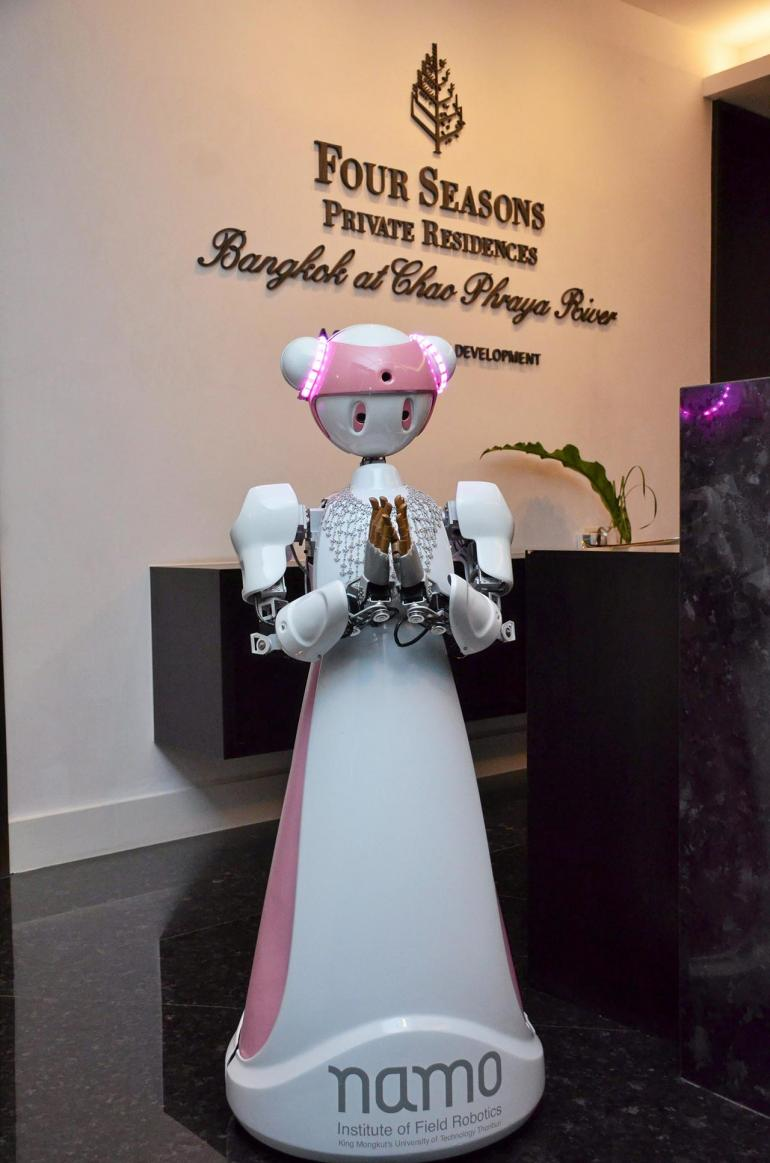
\includegraphics[width=\textwidth]{chapter2/images/namo.jpg}
        \caption{หุ่นยนต์ประชาสัมพันธ์นะโม}
        \label{fig:namo}
    \end{subfigure}
    \hfill
    \begin{subfigure}[b]{0.3\textwidth}
        \centering
        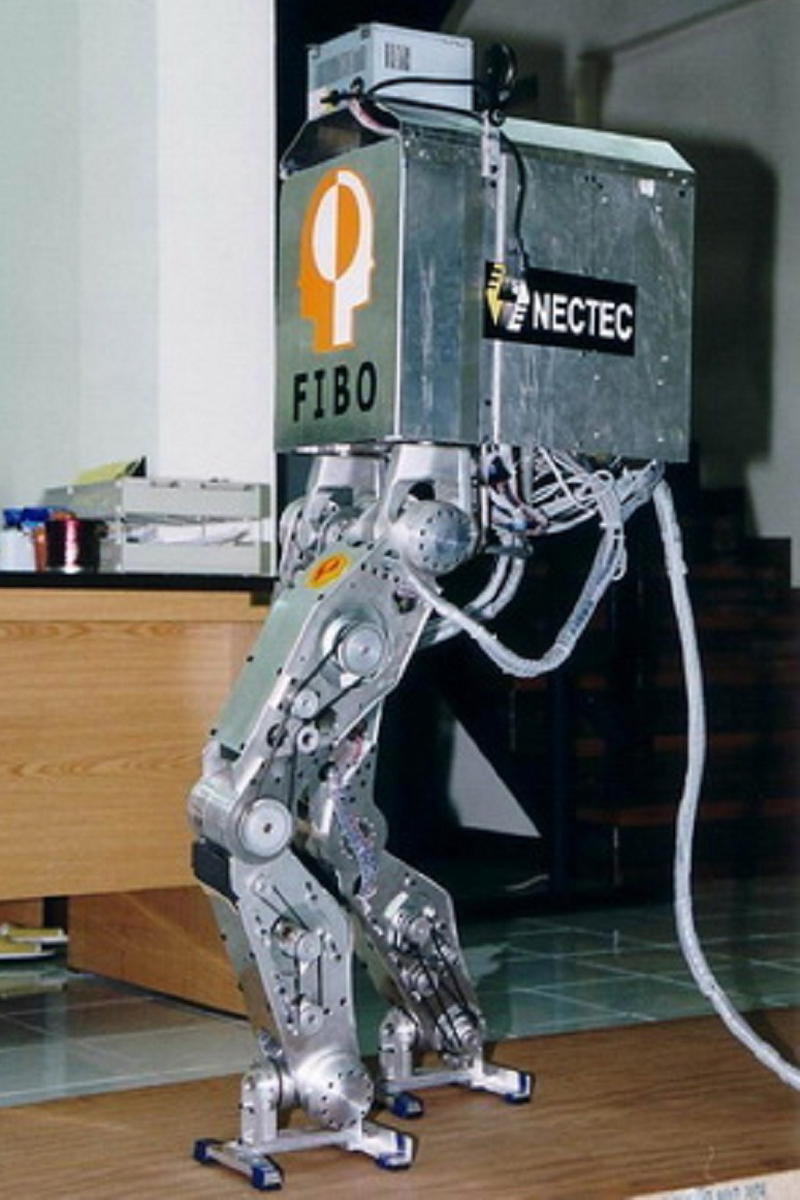
\includegraphics[width=\textwidth]{chapter2/images/ส้มจุก.jpg}
        \caption{หุ่นยนต์เดินสองขาส้มจุก}
        \label{fig:somjook}
    \end{subfigure}
    \hfill
    \begin{subfigure}[b]{0.3\textwidth}
        \centering
        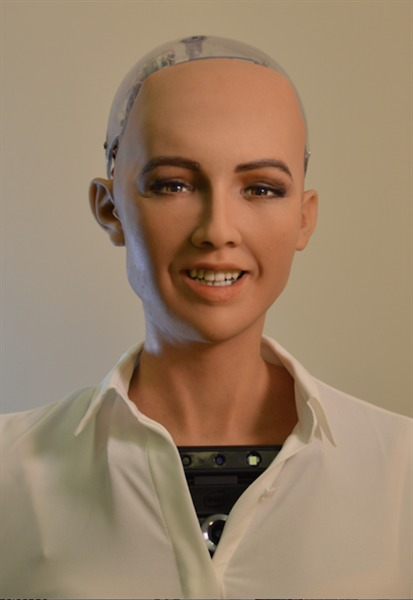
\includegraphics[width=\textwidth]{chapter2/images/โซเฟีย.jpg}
        \caption{หุ่นยนต์แอนดรอยด์โซเฟีย}
        \label{fig:sophia}
    \end{subfigure}
    \caption{แสดงความแตกต่างของหุ่นยนต์ฮิวมานอยด์แต่ละประเภท}
    \label{fig:diff_humanoid}
\end{figure}

งานวิจัยทางด้านหุ่นยนต์ฮิวมานอยด์จากอดีตจนถึงปัจจุบันส่วนใหญ่จะเป็นการพัฒนาความสามารถของการเดินของหุ่นยนต์
เช่น เริ่มต้นจากแรกสุดจะเป็นการพัฒนาให้หุ่นยนต์สามารถเดินหน้าได้ ต่อมาก็เพิ่มความสามารถให้หุ่นยนต์สามารถเดินบนพื้นเอียง พื้นขรุขระ
เดินเลี้ยวซ้ายขวา เดินขึ้นลงบันได ฯลฯ เป็นต้น นอกจากนี้ยังมีการพัฒนาปรับปรุงสมดุลของการเดินแบบสองขาอีกด้วย สมดุลของการเดินสามารถแบ่งได้สองแบบหลัก
คือ การเดินแบบสมดุลสถิต และการเดินแบบสมดุลพลวัต งานในยุคแรกนั้นจะพัฒนาให้เดินได้แบบสมดุลสถิต ต่อมาเป็นสมดุลกึ่งพลวัต
และเป็นสมดุลพลวัต การพัฒนาตัวควบคุมการเดินของหุ่นยนต์ จำเป็นที่จะต้องใช้ความรู้ทางด้านกลศาสตร์ค่อนข้างมาก มีการใช้สมการที่มีความซับซ้อน

Zheng และคณะ (1988) พัฒนาหุ่นยนต์สองขาที่สามารถเดินบนพื้นราบได้ ให้สามารถเดินต่อเนื่องไปบนพื้นเอียงได้ด้วย
พื้นเอียงที่ใช้มีลักษณะเป็นพื้นเอียงขึ้น หุ่นยนต์ที่ใช้ในงานนี้มีข้อต่อสะโพก (hip), ข้อเท้า (ankle) และลำตัว (torso) มีเซนเซอร์วัดแรงกด (force sensor)
ติดตั้งอยู่ที่ปลายเท้าและส้นเท้าแต่ละข้างเพื่อใช้วัดตำแหน่งของน้ำหนักโดยรวม (center of gravity) ของหุ่นยนต์ การเดินของงานวิจัยจะพิจารณาเฉพาะการเดินในแนวหน้าหลัง
โดยมีหลักการคือ การเดินบนพื้นเอียงโดยที่หุ่นยนต์ยังเดินในท่าทางเหมือนกับตอนที่เดินบนพื้นราบจะทำให้น้ำหนักโดยรวมของหุ่นยนต์เลื่อนไปข้างหลัง
ดังนั้นการที่หุ่นยนต์ขยับลำตัวไปด้านหน้าจำทำให้น้ำหนักโดยรวมของหุ่นยนต์กลับมาอยู่ตรงกลางของพื้นที่รับน้ำหนักเหมือนเดิม
ซึ่งจะทำให้หุ่นยนต์มีความสมดุลได้ ดั้งนั้นข้อมูลที่ได้จากหน่วยวัดแรงกดที่เท้าจะถูกนำมาคำนวณตลอดการเดินเพื่อใช้ในการปรับเปลี่ยนมุมการขยับของลำตัว
การเดินบนพื้นราบเป็นแบบสมดุลสถิตและการเดินบนพื้นเอียงก็ยังคงเป็นแบบสมดุลสถิตเช่นกัน

Inaba และคณะ (1995) สร้างหุ่นยนต์เลียนแบบลิง (ape-like biped) ประกอบด้วยสองมือและสองขา มีการเดินแบบสมดุลสถิต
งานวิจัยนี้มีความคิดว่านอกจากการทำให้หุ่นยนต์สองขาเดินได้โดยไม่ล้มแล้ว ควรจะทำหุ่นยนต์ที่สามารถลุกขึ้นเองได้หลังจากที่ล้มแล้วด้วย
ดังนั้นในงานนี้ หุ่นยนต์ถูกพัฒนาให้สามารถเดิน เมื่อล้มแล้วก็สามารถพลิกตัวและลุกขึ้นมาเดินให้ได้

Kun และ Miller (1996) ได้นำโครงข่ายประสาทเทียม มาประยุกต์ใช้ในการปรับเปลี่ยนท่าทางการเดินโดยอัตโนมัติของหุ่นยนต์สองขา
การที่หุ่นยนต์สามารถปรับเปลี่ยนท่าทางได้โดยอัตโนมัตินี้มีประโยชน์ทำให้หุ่นยนต์เดินได้บนพื้นผิวหลากหลายลักษณะมากขึ้น
ในงานนี้พิจารณาท้ังสมดุลในแนวหน้าหลัง (sigittal plane) และแนวซ้ายขวา (frontal plane) และการเดินของหุุ่นยนต์เป็นแบบสมดุลพลวัต
หลักการทำงานประกอบด้วยตัวสร้างท่าทางการเดินหนึ่งตัว และตัวปรับท่าทางการเดินทั้งแนวหน้าหลังและซ้ายขวาอีกหนึ่งตัว
โดยค่าการปรับเปลี่ยนนั้นจะได้มาจาก แรงกดที่เท้า ความยาวการก้าวเท้า ความสูงของการยกเท้า เป็นต้น นอกจากนี้
ในปีถัดมาทั้งสิงได้ใช้หลักการที่ใช้ในงานนี้ไปใช้กับการเดินของหุ่นยนต์อีกตัว (Kun and Miller, 1997)

Hirai และคณะ (1998) พัฒนาหุ่นยนต์ฮิวมานอยด์ ซึ่งตัวหุ่นยนต์มีความคล้ายมนุษย์มาก สามารถเดินได้อย่างราบลื่นคล้านมนุษย์มากที่สุด
เช่น สามารถเดินได้ในพื้นผิวชนิดต่างๆ เดินได้บนพื้นเอียงขึ้นเอียงลง เดินขึ้นลงบันได้ได้ เดินเข็นรถได้ เป็นต้น การเดินในทุกสถานการณ์เป็นการเดินแบบสมดุลพลวัต
หุ่นยนต์สามารถเดินได้ด้วยความเร็วสูงสุด 4.7 กิโลเมตรต่อชั่วโมง หุ่นยนต์ประกอบไปด้วย แขนข้างละ 9 องศาอิสระ ขาข้างละ 6 องศาอิสระ
ที่บริเวณหัวมีกล้องติดตั้งอยู่ 4 ตัว นอกจากนี้ยังมีอุปกรณ์ที่ใช้ในการรักษาสมดุลอื่นๆ อีกได้แก่ IMU ที่ติดตั้งบริเวณลำตัว และ Force sensor ที่ติดที่เท้าทั้งสองข้าง

องค์ประกอบของหุ่นยนต์ทั่วไปจะประกอบไปด้วยกระบวนการตอบสนองต่างๆที่เป็นระบบ
ซึ่งเราสามารถจำแนกกาออกเป็นส่วนหลักๆได้สามส่วนคือ ส่วนการรับรู้ ส่วนการประมวลผล
และส่วนการขับเคลื่อน ทั้งหมดเมื่อนำมารวมเข้าด้วยกันแล้ว เราสามารถที่จะควบคุมการทำงานของหุ่นยนต์ฮิวมานอยด์ได้

\begin{figure}[ht]
    \centering
    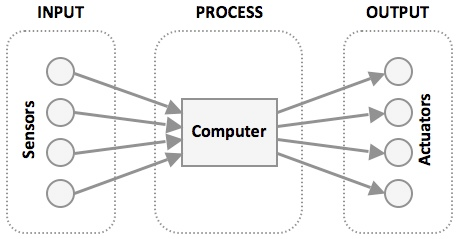
\includegraphics[width=0.45\textwidth]{chapter2/images/humanoid_combine.png}
	\caption{องค์ประกอบหลักการทำงานของหุ่นยนต์ฮิวมานอยด์}
    \label{fig:humanoid_combine}
\end{figure}

\clearpage
\subsubsection*{การรับรู้ของหุ่นยนต์ฮิวมานอยด์}
การรับรู้ของหุ่นยนต์ฮิวมานอยด์นั้นมีความยากมากกว่าหุ่นยนต์ชนิดอื่นๆเพราะหุ่นยนต์จะมีการเคลื่อนที่ และการเคลื่อนที่นั้นทำให้เซนเซอร์โดนรบกวนได้
ยกตัวอย่างเช่น ภาพที่ได้จากกล้องนั้นอาจจะเบลอได้ถ้าความเร็วของชัตเตอร์ช้าเกินไป หรือว่าภาพเปลี่ยนขณะที่กำลังกดชัตเตอร์
ข้อมูลตำแหน่งของตัวเองก็มีความแน่นอนที่น้อยกว่าหุ่นยนต์เคลื่อนที่ด้วยล้อ เพราะเซนเซอร์ที่วัดตำแหน่งเทียบกับเฟรมโลกไม่มีความเสถียร
หุ่นยนต์ที่เคลื่อนที่ด้วยล้อปกติถ้าติดกล้อง ตัวกล้องจะมีความสูงจากพื้นคงที่ แต่หุ่นยนต์ฮิวมานอยด์ไม่ใช่ โดยหุ่นยนต์ฮิวมานอยด์นั้นจะต้องมีการคำนวณ
forward kinematics จากเท้าที่สัมผัสกับพื้นมายังกล้องเพื่อหาตำแหน่งและการหมุนของกล้อง ส่วนการวัดตำแหน่งของตัวหุ่นยนต์นั้น
โดยทั่วไปแล้วจะใช้เซนเซอร์ inertia measurement unit (IMU) และเซนเซอร์ Encoders สำหรับหาตำแหน่งของข้อต่อต่างๆ
ปกติจะติดเซนเซอร์ IMU ไว้ที่ลำตัวของหุ่นยนต์ใกล้ๆกับ center of mass ของหุ่นยนต์ ส่วน Encoder นั้นจะติดไว้ที่ข้อต่อของหุ่นยนต์

\subsubsection*{การประมวลผลของหุ่นยนต์ฮิวมานอยด์}
ในปัจจุบันนี้หุ่นยนต์ฮิวมานอยด์มีความสามารถในการคำนวณที่สูงมากเมื่อเทียบกับเมื่อก่อน บอร์ดที่เราสามารถเห็นได้โดยทั่วไปเช่น
Raspberry Pi, Odroid, Intel NUCs ซึ่งตัวบอร์ดมีขนาดเล็กจึงทำให้เข้าไปอยู่ในตัวของหุ่นยนต์ได้ แถมบอร์ดพวกนี้ยังมี GPUs
และ CPU หลายคอร์อีกด้วย บางครั้งก็มีคนที่เอาพวกบอร์ดพวกนี้มาทำงานร่วมกันหลายๆตัว ประมวลผลแบบ pararell เพื่อที่จะเพิ่มประสิทธิภาพในการประมวลผล
โดยเชื่อมต่อระหว่างกันผ่าน Ethernet network 

\subsubsection*{การขับเคลื่อนของหุ่นยนต์ฮิวมานอยด์}
หุ่นยนต์ฮิวมานอยด์ส่วนใหญ่จะมีข้อต่ออยู่หลายๆจุด แต่ละข้อต่อจะมีตัวขับเคลื่อน ตัวขับเคลื่อนมีอยู่หลักๆสองแบบคือ
แบบกล้ามเนื่อของมนุษย์ และแบบมอเตอร์ที่ติดตรงที่ข้อต่อเลย ที่นิยมใช้คือแบบมอเตอร์ที่ติดที่ข้อต่อเลย เพราะทำให้ตัวของหุ่นยนต์มีขนาดเล็ก
ใช้พื้นที่น้อย การใช้เส้นเอ็นดึงนั้นจะการจะทำให้ข้อต่อไปยังตำแหน่งที่ต้องการได้ยากกว่า ตัวขับเคลื่อนนั้นต้องการแรงมากน้อยขึ้นอยู่กับ
น้ำหนักของตัวหุ่นยนต์ เพื่อที่จะทำให้หุ่นยนต์นั้นยังยืนได้


\clearpage
\subsection{ทฤษฏีที่เกี่ยวข้องกับมนุษย์}
\subsubsection{การวิเคราะห์การเดินของมนุษย์}
การเคลื่อนที่ของหุ่นยนต์ฮิวมานอยด์นั้นจะเลียนแบบมาจากการเดินของมนุษย์
ดั้งนั้นการวิเคราะห์ลักษณะการเดินของมนุษย์ จะเป็นการศึกษาเพื่อทำความเข้าใจถึงธรรมชาติการเดิน
ก่อนนำไปทำการออกแบบกลไกทางกลและระบบควบคุมของหุ่นยนต์ฮิวมานอยด์
การก้าวเดินของมนุษย์โดยปกติแล้ว จะมีลักษณะเป็นวัฏจักร วนซ้ำไปเรื่อยๆ ในทิศทางที่ต้องการจนกว่าจะทำการหยุดเดิน
การทรงตัวในระหว่างการยืนหรือการเดินนั้น เป็นไปตามสัญชาติญาณซึ่งเกิดจากการรักษาความสมดุลของระดับน้ำในหู\footnote{ Rose, J. and Gamble, J., 1993, Human Walking, Williams $\&$  Wilkins, Philadelphia, pp. 10-44. }
ส่งสัญญาณผ่านเส้นประสาทไปยังกล้ามเนื้อส่วนต่างๆ ที่ทำหน้าที่ให้เกิดการเคลื่อนที่

การเคลื่อนที่ของมนุษย์ในการเดินไปข้างหน้าสามารถแบ่งออกเป็นช่วงต่างๆดังนี้
\begin{figure}[!ht]
	\centering
	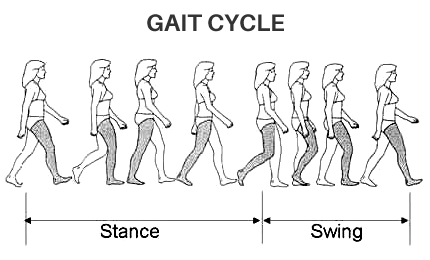
\includegraphics[width=0.65\textwidth]{chapter2/images/gaitcycle.png}
	\caption{วัฏจักรการเดินของมนุษย์}
	\label{fig:human_gait_cycle}
\end{figure}
\begin{enumerate}[label=\arabic*., leftmargin=1.5cm]
	\item ช่วงเริ่มการวางเท้าเพื่อเข้าสู่ช่วงเริ่มต้นเหวี่ยงเท้า เป็นช่วงที่เท้าเกิดการกระแทกลงบนพื้นหลังจากทำการเหวี่ยงมาจากด้านหลัง
	      โดยธรรมชาติมนุษย์จะทำการวางส้นเท้าลงเพื่อลดแรงกระแทกที่เกิดขึ้นในช่วงนี้
	      ดังนั้นทางกายภาพในส่วนของส้นเท้ามนุษย์จึงมีลักษณะอ่อนนุ่ม
	\item ช่วงเริ่มต้นเหวี่ยงเท้าเพื่อเข้าสู่ช่วงเหวี่ยงเท้า หลังจากทำการวางส้นเท้าลงกับพื้นแล้ว ข้อเข้าจะปรับมุมเพื่อให้ฝ่าเท้าแนบพื้นสนิท
	      ขณะเดียวกันขาอีกข้างจะยกสูงขึ้นเพื่อถ่ายเทน้ำหนักไปยังเท้าที่เพิ่งวางลง
	\item ช่วงเหวี่ยงเท้า เป็นช่วงที่ขาหนึ่งยกลอยอยู่ในอากาศและขาที่วางแนบกับพื้นจะรองรับน้ำหนักทั้งหมดของร่างกาย
	\item ช่วงเตรียมการวางเท้า เป็นช่วงที่ขาข้างที่ลอยอยู่เหวี่ยงไปข้างหน้าเพื่อเตรียมเข้าสู่ช่วงรองรับ 
	      ในขณะเดียวกันขาที่รับน้ำหนักอยู่จะทำการผลักตัวเพื่อเริ่มทำการถ่ายเทน้ำหนักไปข้างหน้า
\end{enumerate}

\clearpage
\subsubsection{การวิเคราะห์องศาอิสระของมนุษย์}
การที่มนุษย์สามารถเคลื่อนที่ได้เป็นผลเนื่องมาจากการเคลื่อนที่ของข้อต่อต่างๆ ซึ่งประกอบไปด้วย ข้อต่อส่วนสะโพก ส่วนหัวเข่า และส่วนข้อเท้า
แรงบิดที่เกิดขึ้นของแต่ละข้อต่อมีความสัมพันธ์ต่อกัน ส่งผลให้เกิดเสถียรภาพในการเดินของมนุษย์
เมื่อวิเคราะห์ลักษณะโครงสร้างในแต่ละส่วน พบว่าข้อต่อส่วนสะโพกมีลักษณะเป็นทรงกลม 
ทำให้ข้อต่อส่วนสะโพกสามารถหมุนได้ 3 องศาอิสระ ส่วนหัวเข่าของมนุษย์มีจุดต่อของข้อที่มีลักษณะเป็นทรงกลม
สองลูกประกอบเข้าด้วยกันทำให้การเคลื่อนที่ถูกบังคับให้สามารถเคลื่อนที่ได้เพียง 1 องศาอิสระ
ในส่วนของข้อเท้ามีลักษณะการเคลื่อนที่เหมือนสะโพกคือสามารถเคลื่อนที่ได้ 3 องศาอิสระ

จากทั้งหมดที่ได้ทำการวิเคราะห์มาข้างต้นพบว่าในขาหนึ่งข้างของมนุษย์ประกอบด้วย 7 องศาอิสระ
ซึ่งส่งผลให้การเคลื่อนที่ของมนุษย์มีความคล่องแคล่วสูง แต่ในทางออกแบบกลไกการเดินและการควบคุม
ของหุ่นยนต์สองขาถือว่ามีจำนวนองศาอิสระเกินความจำเป็นในการเคลื่อนที่บนปริภูมิ (space) และยากต่อการควบคุม
(underactuated) ดังนั้นการกำหนดจำนวนองศาอิสระเพื่อให้หุ่นยนต์เดินได้เสมือนมนุษย์จึงมีผลในการออกแบบกลไกทางกลและการควบคุมของหุ่นยนต์สองขา 

\begin{table}[!ht]
	\centering
	\begin{tabular}{|c|c|c|c|}
		\hline
		{ข้อต่อ}&{องศาอิสระ}&\multicolumn{2}{c|}{องศาการหมุน}\\
		\cline{3-4}
		{}                                     & {}         & {สูงสุด} & {ต่ำสุด} \\
		\hline
		\multirow{3}{*}{หัว}             & $\theta_x$ & +60                  & -30                  \\
		\cline{3-4}
		                                       & $\theta_y$ & +70                  & -70                  \\
		\cline{3-4}
		                                       & $\theta_z$ & +80                  & -80                  \\
		\hline
		\multirow{3}{*}{หลัง}          & $\theta_x$ & +30                  & -30                  \\
		\cline{3-4}
		                                       & $\theta_y$ & +55                  & -55                  \\
		\cline{3-4}
		                                       & $\theta_z$ & +45                  & -45                  \\
		\hline
		\multirow{3}{*}{หัวไหล่} & $\theta_x$ & +180                 & -80                  \\
		\cline{3-4}
		                                       & $\theta_y$ & +45                  & -135                 \\
		\cline{3-4}
		                                       & $\theta_z$ & +30                  & 0                    \\
		\hline
		{ศอก}                            & $\theta_x$ & 0                    & -155                 \\
		\hline
		\multirow{3}{*}{สะโพก}       & $\theta_x$ & +120                 & -40                  \\
		\cline{3-4}
		                                       & $\theta_y$ & +40                  & -50                  \\
		\cline{3-4}
		                                       & $\theta_z$ & +60                  & -50                  \\
		\hline
        {หัวเข่า}                & $\theta_x$ & 0                    & -130                 \\
        \hline
		\multirow{3}{*}{ข้อเท้า} & $\theta_x$ & +30                  & -60                  \\
		\cline{3-4}
		                                       & $\theta_y$ & +45                  & -20                  \\
		\cline{3-4}
		                                       & $\theta_z$ & +20                  & -60                  \\
		\hline
	\end{tabular}
	\caption{ความสามารถในการหมุนของแต่ละข้อต่อของมนุษย์}
	\label{tab:human_joint_limit}
\end{table}

ผู้เขียนได้ข้อสรุปในการออกแบบขาหนึ่งข้างของหุ่นยนต์ให้มีองศาอิสระเท่ากับ 6 องศาอิสระ และได้ใช้ดิจิตอลเซอร์โวของบริษัท Robotis เป็นตัวขับเคลื่อนข้อต่อ
เนื่องจากภายในเซอร์โวมีตัวรับรู้สถานะของตัวเอง และเซอร์โวนี้ถูกออกแบบมาให้สามารถติดตั้ง และสั่งการได้ง่าย



\clearpage
\subsection{ทฤษฏีที่เกี่ยวข้องกับหุ่นยนต์ฮิวมานอยด์}
\subsubsection{ส่วนประกอบของหุ่นยนต์ฮิวมานอยด์}
\begin{figure}[ht]
	\centering
	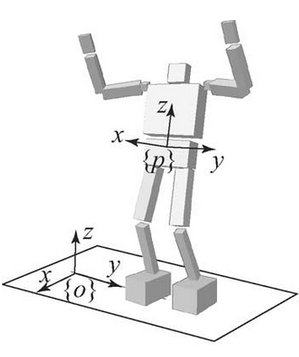
\includegraphics[width=0.4\textwidth]{chapter2/images/robot_component.png}
	\caption{ส่วนประกอบของหุ่นยนต์ฮิวมานอยด์}
	\label{fig:robot_component}
\end{figure}
หุ่นยนต์ฮิวมานอยด์ประกอบด้วยก้านต่อหลายๆก้านที่นำมาต่อกัน ลักษณะโครงสร้างนั้นจะเป็นแบบโซ่เปิด (Open kinematic chain)
และแต่ละก้านต่อจะเชื่อมต่อกันด้วยข้อต่อแบบหมุน เราสามารถแบ่งโครงสร้างของหุ่นยนต์ฮิวมานอยด์ออกเป็นส่วนหลักๆเป็น 2 ส่วน ส่วนแรกคือ
ส่วนก้านต่อของลำตัวหุ่นยนต์ (Torso) ซึ่งเราสามารถที่จะรวมไปถึงส่วนแขนกับหัวด้วย
และในส่วนที่สองคือ ส่วนก้านต่อของขาหุ่นยนต์ (Legs) ซึ่งเป็นส่วนขาของหุ่นยนต์ทั้งสองข้างที่สามารถนำไปที่สัมผัสกับพื้นได้
ทั้งสองก้านต่อนี้ถูกเชื่อมต่อกันด้วยส่วนของสะโพก (Hip) ที่อยู่ระหว่างส่วนลำตัวกับส่วนของขาหุ่นยนต์ ดังรูปที่ \ref{fig:robot_component}

\subsubsection{วัฏจักรการเดินของหุ่นยนต์ฮิวมานอยด์}
วัฏจักรการเดินของหุ่นยนต์ คือ การที่หุ่นยนต์จะต้องมีการถ่ายน้ำหนักไปมาระหว่างเท้าซ้ายและเท้าขวา
มีบางช่วงที่น้ำหนักตกลงบนเท้าข้างใดข้างหนึ่งหรือทั้งสองข้างพร้อมกัน สามารถแบ่งออกเป็นช่วงได้สองช่วง คือช่วงการยืนด้วยขาข้างเดียว
และช่วงการยืนด้วยขาทั้งสองข้าง
\begin{figure}[!ht]
	\centering
	\begin{subfigure}[b]{0.22\textwidth}
		\centering
		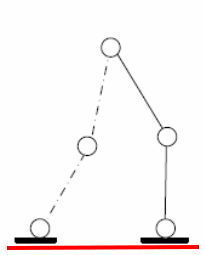
\includegraphics[width=\textwidth]{chapter2/images/doublesupport.png}
		\caption{ยืนด้วยขาสองข้าง}
		\label{fig:robot_walk_1}
	\end{subfigure}
	\hfill
	\begin{subfigure}[b]{0.45\textwidth}
		\centering
		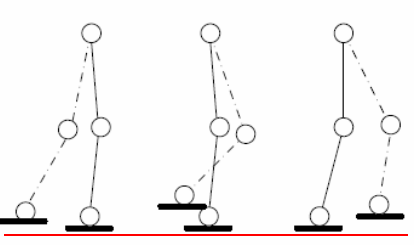
\includegraphics[width=\textwidth]{chapter2/images/singlesupport.png}
		\caption{ยืนด้วยขาข้างเดียว}
		\label{fig:robot_walk_2}
	\end{subfigure}
	\hfill
	\begin{subfigure}[b]{0.22\textwidth}
		\centering
		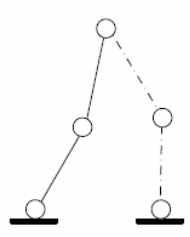
\includegraphics[width=\textwidth]{chapter2/images/doublesupport2.png}
		\caption{ยืนด้วยขาสองข้าง}
		\label{fig:robot_walk_3}
	\end{subfigure}
	\caption{วัฐจักรการเดินของหุ่นยนต์ฮิวมานอยด์}
	\label{fig:robot_walk_phase}
\end{figure}

\clearpage
\paragraph*{1) การยืนด้วยขาข้างเดียว :}
เป็นช่วงที่มีเท้าของหุ่นยนต์สัมผัสพื้นเพียงข้างเดียว ส่วนเท้าอีกข้างของหุ่นยนต์จะถูกยกลอยจากพื้น
โดยที่ไม่มีส่วนใดๆของขาข้างนั้นสัมผัสกับพื้นเลย ช่วงนี้จะเกิดขึ้นเมื่อมีการแกว่งเท้าจากข้างหลังไปข้างหน้า
ดังจากภาพที่ \ref{fig:robot_walk_2}

\paragraph*{2) การยืนด้วยขาสองข้าง :}
เป็นช่วงที่เท้าทั้งสองข้างของหุ่นยนต์สัมผัสกับพื้น ช่วงนี้จะเกิดตั้งแต่หุ่นยนต์วางเท้าขณะที่ส้นเท้าแตะกับพื้น
ไปจนถึง ปลายเท้าของขาอีกข้างหลุดออกจากพื้น

การเดินได้โดยไม่ล้มนั้น ตัวหุ่นยนต์จะต้องรักษาสมดุลของการเดินให้ได้ตลอดช่วงเวลาของการเดิน
ซึ่งสมดุลของการเดินแบบสองขาสามารถแบ่งตามลักษณะการเดินและการถ่ายน้ำหนักได้เป็น 2 รูปแบบหลัก คือ 
การเดินแบบสมดุลสถิต (static balance walking) และ การเดินแบบสมดุลพลวัต (dynamic balance walking)

\subsubsection{การสร้างและการควบคุมการเดินแบบสมดุลสถิต}
การเดินของหุ่นยนต์ในลักษณะนี้ จุดศูนย์กลางมวลตัวหุ่นยนต์จะไม่มีการเคลื่อนไหวออกนอกบริเวณฐานรับน้ำหนัก (Supporting Area)
ตลอดช่วงเวลาการเดิน ไม่ว่าจะเป็นช่วงเวลาที่รับน้ำหนักด้วยเท้าข้างเดียวหรือทั้งสองข้างก็ตาม หมายความว่า โครงสร้างของหุ่นยนต์จะไม่ล้มแน่นอน
เนื่องจากการสร้างรูปแบบการเดินด้วยวิธีนี้จะควบคุมให้ตำแหน่งของจุดรวมมวล (CoM) อยู่ภายในพื้นที่ฐานรับน้ำหนักของหุ่นยนต์ตลอดเวลา

\begin{figure}[ht]
	\centering
	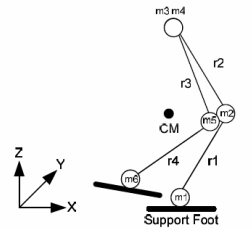
\includegraphics[width=0.4\textwidth]{chapter2/images/cominsupportpolygon.png}
	\caption{การควบคุมตำแหน่งของจุดรวมมวลให้อยู่ในพื้นที่ฐาน}
	\label{fig:robot_com_support}
\end{figure}

ข้อดีของการสร้างและควบคุมการเดินของหุ่นยนต์ด้วยวิธีนี้คือ สามารถสร้างรูปแบบการเดินได้โดยที่มีความซับซ้อนไม่มากนัก
สามารถสั่งให้หุ่นยนต์หยุดค้างในท่าทางใดๆก็ได้ตลอดเวลาโดยหุ่นยนต์ไม่ล้ม หุ่นยนต์ที่มีฝ่าเท้าใหญ่จะทำให้ง่ายต่อการก้าวเดินมากขึ้น
นอกจากการควบคุมการก้าวขาแล้วอาจเพิ่มการควบคุมส่วนลำตัวเพิ่มเติม เพื่อเป็นการเพิ่มเสถียรภาพในการเดินและการถ่ายเทน้ำหนัก
โดยที่อาจจะมีการเพิ่มเซนเซอร์วัดแรงที่ฝ่าเท้าเพื่อตรวจสอบการกระจายแรงกดที่ฝ่าเท้า เพื่อตรวจสอบว่าตำแหน่งของจุดรวมน้ำหนักอยู่บนพื้นที่ฝ่าเท้าหรือไม่
หรือเพื่อตรวจสอบเสถียรภาพของการเดินเพื่อแก้ไขท่าทางการเดินไม่ให้เกิดการล้ม

ข้อเสียของการควบคุมการเดินด้วยวิธีนี้คือ หุ่นยนต์จะใช้เวลาในการก้าวเดินมาก ใช้พลังงานในการเดินมากกว่าการเดินแบบสมดุลพลวัต
และท่าทางที่ได้จะมีความแตกต่างจากท่าทางการเดินของมนุษย์

\subsubsection{การสร้างและการควบคุมการเดินแบบสมดุลพลวัต}
การสร้างรูปแบบการเดินและควบคุมการเดินในลักษณะนี้ท่าทางการเดินของหุ่นยนต์นั้นจะคล้ายกับการเดินของมนุษย์มากกว่าแบบสถิต
เนื่องจากมีหลักการในการสร้างท่าทางที่เหมือนกับการเดินของมนุษย์ซึ่งมีขั้นตอนดังนี้คือ เอียงตัวให้ล้มไปในทิศทางที่ต้องการเดิน
เมื่อเริ่มเกิดการล้มขึ้นหุ่นยนต์จะเปลี่ยนตำแหน่งการวางเท้าไปยังตำแหน่งใหม่ เพื่อปรับให้โครงสร้างเข้าสู่สภาวะสมดุลอีกครั้ง

โดยธรรมชาติแล้วมนุษย์มีการถ่ายน้ำหนักในขณะที่เคลื่อนที่หรือยืนอยู่กับที่เพื่อรักษาสมดุลของท่าทางนั้นไว้
แต่หากการถ่ายโอนน้ำหนักนั้นเกิดสภาวะไม่สมดุล ร่างกายจะปรับสภาพโดยการเคลื่อนตำแหน่งของเท้าซึ่งเป็นพื้นที่ฐานออกจากเดิมไปยังตำแหน่งใหม่
เพื่อรักษาสมดุลไว้ หลักการดังกล่าวถูกนำมาใช้กับการควบคุมการเดินของหุ่นยนต์ฮิวมานอยด์ ในขณะที่หุ่นยนต์กำลังเคลื่อนไหว
ผลจากแรงเฉื่อยของการเคลื่อนที่และผลจากแรงดึงดูดของโลกมีผลต่อการเพิ่มและลดความเร่งให้การเดินของหุ่นยนต์
แรงเหล่านี้เรียกว่าแรงเฉื่อยรวมของการเคลื่อนที่ และเมื่อเท้าหุ่นยนต์สัมผัสกับพื้นจะได้รับผลกระทบของแรงนี้ เรียกว่า
แรงปฏิกิริยาจากพื้น

การตัดกันระหว่างแรงปฏิกิริยาจากพื้นและแนวแรงเฉื่อยรวม ตำแหน่งนั้นหากทำให้โมเมนต์เท่ากับศูนย์
เรียกจุดตัดนี้ว่าจุดโมเมนต์ศูนย์ ($ZMP_{robot}$) และจุดที่แรงปฏิกิริยาลงสู่พื้นว่า จุดปฏิกิริยาพื้นฐาน 
ท่าทางการเดินของหุ่นยนต์จะถูกกำหนดและถูกส่งให้กับชุดควบคุมข้อต่อจุดต่างๆของหุ่นยนต์ โดยให้สอดคล้องกับแรงเฉื่อยรวมที่เกิดขึ้นจากการคำนวณ
เรียกว่าแรงเฉื่อยรวมเป้าหมาย และจุดโมเมนต์ศูนย์ที่ได้จากการคำนวณเรียกว่าจุดโมเมนต์ศูนย์เป้าหมาย ($ZMP_{target}$)
เมื่อหุ่นยนต์เกิดสมดุลในขณะที่ทำการเดินได้อย่างสมบูรณ์ แนวแกนของแรงเฉื่อยรวมเป้าหมายและแรงปฏิกิริยาที่พื้นจะเป็นตำแหน่งเดียวกัน
แต่ในขณะที่หุ่นยนต์เดินผ่านพื้นผิวที่มีความขรุขระหรือไม่เรียบตำแหน่งสองจุดดังกล่าง จะไม่ใช่ตำแหน่งเดียวกันทำให้หุ่นยนต์เกิดการล้มได้
แรงที่ทำให้เกิดการล้มนี้เกิดจากตำแหน่งของจุดโมเมนต์ศูนย์และตำแหน่งแรงปฏิกิริยารวมที่พื้นไม่ตรงกัน ซึ่งเป็นสาเหตุหลักที่ทำให้เกิดความไม่สมดุลขึ้น
และเมื่อหุ่นยนต์เสียสมดุลระบบที่จะสามารถป้องกันการล้มและทำให้หุ่นยนต์เดินต่อไปได้อย่างต่อเนื่องคือ ระบบควบคุมแรงปฏิกิริยา
ระบบควบคุมจุดโมเมนต์ศูนย์ และระบบควบคุมการวางเท้า

\begin{figure}[!ht]
	\centering
	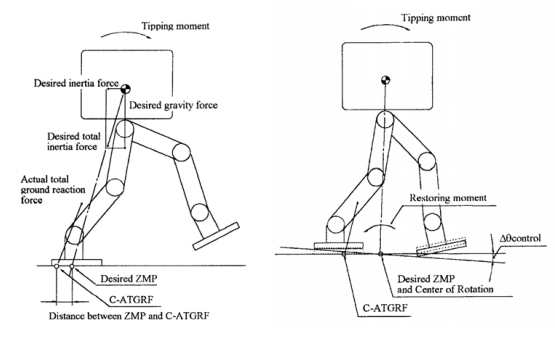
\includegraphics[width=0.7\textwidth]{chapter2/images/zmpdynamicwalking.png}
	\caption{การควบคุมตำแหน่งของจุดโมเมนต์ศูนย์ให้ตรงกับแรงปฏิกิริยารวม}
	\label{fig:robot_zmp_support}
\end{figure}

อย่างไรก็ตาม การสร้างท่าทางการเดินในลักษณะนี้ต้องใช้สมการในการคำนวณที่ซับซ้อนมาก
เนื่องจากต้องหาความสัมพันธ์ระหว่างองค์ประกอบหลายส่วน เช่น น้ำหนักของโครงสร้างในแต่ละส่วน 
แรงบิดที่แต่ละข้อต่อ และโมเมนต์โดยรวมของระบบ นอกจากนี้ยังต้องใช้อุปกรณ์การตรวจวัดต่างๆ เช่น เซนเซอร์วัดแรง
เซนเซอร์วัดมุม เซนเซอร์วัดแรงบิด ติดตั้งตามจุดต่างๆของโครงสร้างเพื่อวัดค่าออกมา ก่อนที่จะทำการคำนวณตำแหน่ง
และสร้างท่าทางการเดินของหุ่นยนต์ฮิวมานอยด์ ท่าทางการเดินที่ได้จากการควบคุมด้วยวิธีนี้ จะมีความคล้ายคลึงกับท่าทางการเดินของมนุษย์มาก

\subsubsection{จุดศูนย์กลางมวลของหุ่นยนต์}
หากต้องการให้หุ่นยนต์สามารถที่จะทรงตัวอยู่ได้โดยไม่ล้มนั้น จึงต้องรู้ตำแหน่งจุดศูนย์กลางมวลของหุ่นยนต์ตลอดเวลา
และต้องให้จุดศูนย์กลางมวลฉายตกในบริเวณฐานรับน้ำหนักของหุ่นยนต์โดยหาจากพื้นที่ที่ฝ่าเท้าสัมผัสกับพื้น
วิธีการนี้เป็นวิธีการทางสถิตศาสตร์

\clearpage
\subsection{ตัวอย่างหุ่นยนต์ฮิวมานอยด์}
\subsection*{Poppy Humanoid}
\begin{figure}[ht]
    \centering
    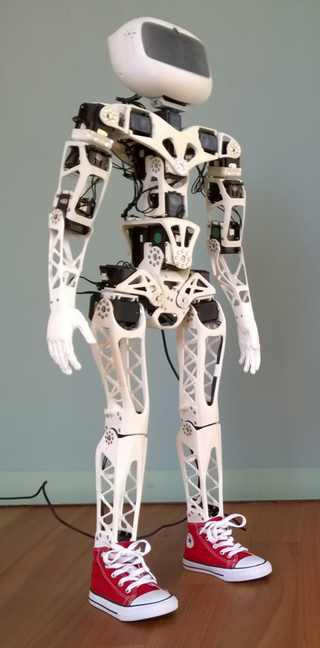
\includegraphics[width=0.35\textwidth]{chapter2/images/PoppyHumanoid1.png}
    \caption{หุ่นยนต์ฮิวมานอยด์ป๊อปปี้}
    \label{fig:poppy_humanoid}
\end{figure}
หุ่นยนต์ฮิวมานอยด์ป๊อปปี้ ถูกสร้างขึ้นมาเพื่อใช้ในงานศิลปะ การวิจัยและการศึกษาโดยเฉพาะ 
หุ่นยนต์ป๊อปปี้ประกอบด้วยส่วนของฮาร์ทแวร์และซอฟแวร์ที่เปิดเป็นโอเพนซอร์ซให้ผู้ที่สนใจสามารถเข้ามาศึกษาได้
โปรแกรมของหุ่นยนต์ใช้โมดูลที่มีชื่อว่า Pypot ที่เป็นส่วนเสริมของภาษา Python ในการพัฒนาซอฟแวร์
ทุกคนสามารถเข้าถึงข้อมูลเชิงเทคนิคของหุ่นยนต์ฮิวมานอยด์ป๊อปปี้ได้ เช่น ส่วนรายละเอียดการทำงาน
คลิปวีดีโอสอนการประกอบ การใช้ระบบจำลอง และการพัฒนาต่างๆผ่านทางเว็บไซต์ http://www.poppy-project.org 
หุ่นยนต์ป๊อปปี้มีส่วนของโครงสร้างที่ผลิตมาจากพลาสติด PLA และ ABS โดยใช้เทคนิคการขึ้นรูปด้วยเครื่องพิมพ์สามมิติ
ตัวขับเคลื่อนข้อต่อต่างๆใช้เป็น Dynamixel Digital Servo และควบคุมคำสั่งของตัวขับเคลื่อนด้วย 
คอมพิวเตอร์ขนาดเล็ก Odroid UX4 ใช้ระบบปฎิบัติการ Ubuntu 14.04 
ตัวของหุ่นยนต์มีความสูง 83 เซนติเมตร น้ำหนัก 3.5 กิโลกรัม 
ใช้เซนเซอร์วัดมุมเอียงเป็น IMU ที่มีองศาอิสระเท่ากับ 9 องศาอิสระ ในการควบคุมเสถียรภาพในการเดินของตัวเอง
มีองศาอิสระหรือจำนวนตัวขับเคลื่อนทั้งหมด 25 องศา ประกอบไปด้วย ขาข้างละ 6 องศาอิสระ แขนข้างละ 4 องศาอิสระ 
ลำตัว 3 องศาอิสระ และ หัว 2 องสาอิสระ

\clearpage
\subsection*{iCub Humanoid}
\begin{figure}[ht]
    \centering
    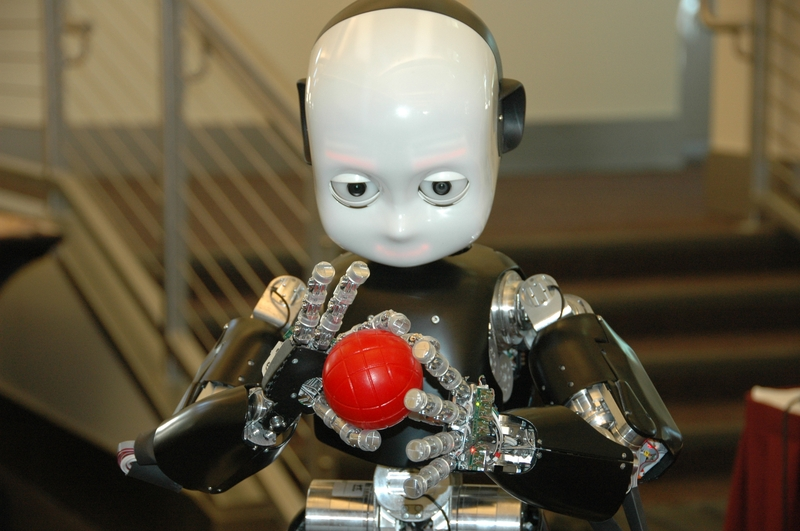
\includegraphics[width=0.6\textwidth]{chapter2/images/icub-1.jpg}
    \caption{หุ่นยนต์ฮิวมานอยด์ไอคัพ}
    \label{fig:icub_humanoid}
\end{figure}
หุ่นยนต์ฮิวมานอยด์ไอคัพ ถูกออกแบบโดยมหาวิทยาลัยหลายแห่งในยุโรปรวมกลุ่มกันขึ้นมาในชื่อ RobotCub
และถูกสร้างขึ้นโดย Istituto Italiano di Tecnologia (IIT) ตัวหุ่นยนต์ไอคัพนั้นมีความสูงอยู่ที่ 1 เมตร
น้ำหนักโดยรวมทั้งหมดประมาณ 22 กิโลกรัม วัสดุที่ใช้ในการสร้างแตกต่างกันไปในแต่ละส่วนของร่างกายโดยจะใช้
aluminum alloy AI6082 สำหรับส่วนที่ต้องรับภาระความเครียดน้อย ใช้ aluminum alloy 7075 (Ergal) สำหรับส่วนที่ต้องรับภาระความเครียดปานกลางถึงสูง
และใช้ Stainless Steel 17-4PH ในส่วนของเพลาข้อต่อต่างๆเพื่อให้มีความแข็งแรงสูง ตัวหุ่นยนต์ถูกออกแบบให้มีลักษณะเหมือนเด็กอายุ 3-4 ขวบ
ควบคุมโดยใช้บอร์ดไมโครคอนโทรเลอร์เป็นรุ่น PC104 Controller ภาษาที่ใช้ในการพัฒนาใช้เป็นภาษา C++ ในการเขียนโปรแกรม
การติดต่อสื่อสารกับตัวขับเคลื่อนหรือมอเตอร์ตามข้อต่อต่างๆ และเซนเซอร์ ผ่านทางโปรโตคอล CAN Bus เพื่อทำให้ใช้สายน้อยลง
ใช้เส้นเอ็นในการส่งถ่ายแรงขับเคลื่อนไปยังส่วนของข้อต่อส่วนมือและไหล่ นิ้วของหุ่นยนต์ถูกร้อยด้วย สายเคเบิลเคลือบ Teflon อยู่ภายใน
และคลายตัวกลับสู่สภาวะสมดุลได้ด้วยแรงของสปริง เซนเซอร์วัดมุมของข้อต่อแต่ละตัวใช้การออกแบบให้มี Hall-effect ติดอยู่
ช่วยในการอ่านค่าของตำแหน่งและความเร็วที่เกิดขึ้นที่ข้อต่อนั้น หุ่นยนต์ไอคัพมีองศาอิสระรวมกันทั้งหมด 53 องศาอิสระ
ประกอบไปด้วย แขนข้างละ 7 องศาอิสระ มือข้างละ 9 องศาอิสระ หัว 6 องศาอิสระ ลำตัว 3 องศาอิสระ และขาข้างละ 6 องศาอิสระ
ในส่วนของหัวจะประกอบไปด้วย กล้องสองตัวเพื่อทำสเตอริโอวิชั่น ไมโครโฟนสำหรับรับเสียงจากสภาพแวดล้อมภายนอก
และไฟแสดงอารมณ์บริเวณปากและคิ้ว หุ่นยนต์นี้ไม่ได้ถูกออกแบบให้มีการทำงานเป็นแบบอัตโนมัติ ซึ่งก็คือตัวหุ่นยนต์นั้นไม่มีแบตเตอรี่ภายในตัว
แต่ใช้แหล่งพลังงานจากภายนอกโดยการส่งเข้าไปผ่านสายเคเบิล และเชื่อมต่อกับอินเทอร์เน็ตผ่านสายแลน (LAN)

\clearpage
\subsection*{Darwin-OP Humanoid}
\begin{figure}[ht]
    \centering
    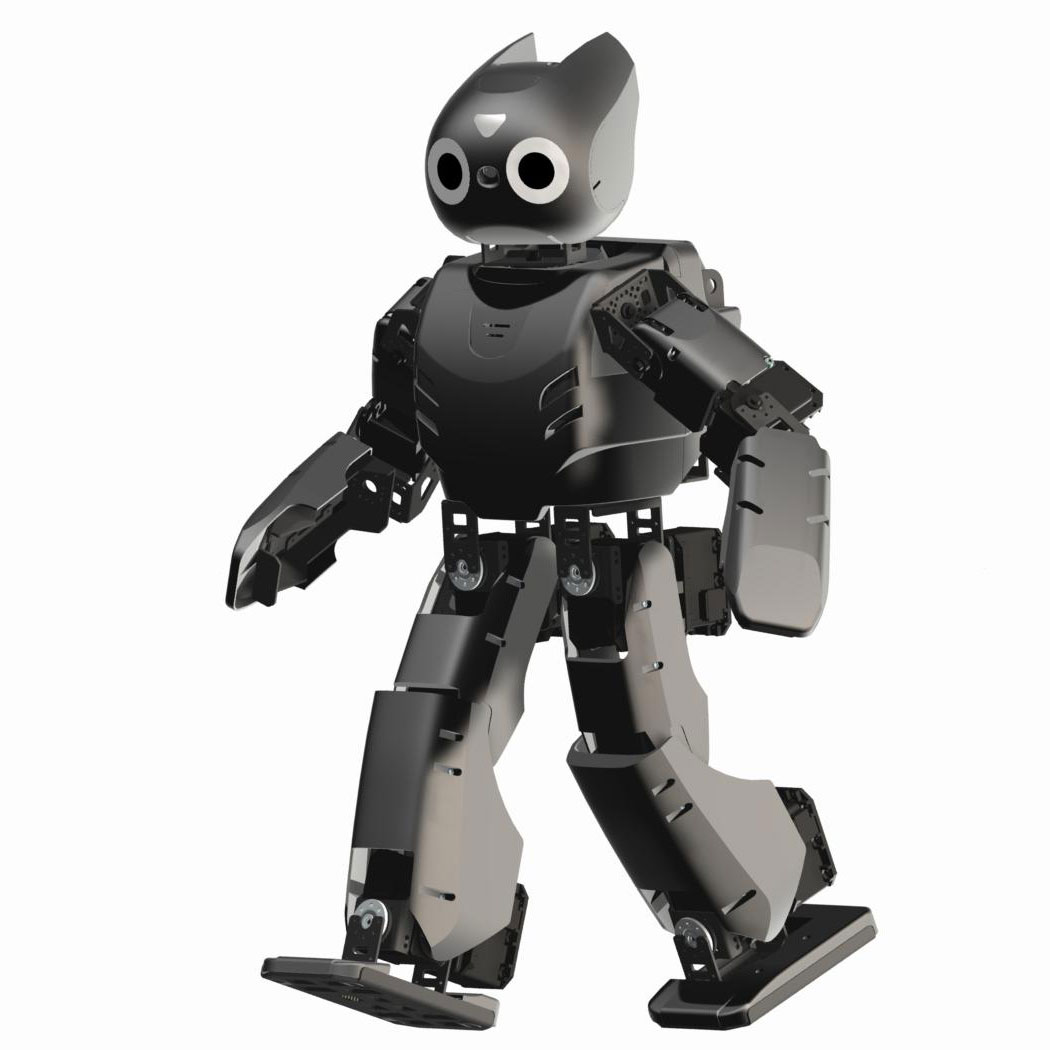
\includegraphics[width=0.55\textwidth]{chapter2/images/Darwin_OP_6.jpg}
    \caption{หุ่นยนต์ฮิวมานอยด์ดาร์วิน}
    \label{fig:darwin_humanoid}
\end{figure}
หุ่นยนต์ฮิวมานอยด์ดาร์วิน (Darwin-OP) เป็นชื่อที่ย่อมาจากคำว่า Dynamic Anthropomorphic Robot
with Intelligence–Open Platform
เป็น OpenSource Platform ที่ถูกออกแบบและพัฒนาโดย Korean robot manufacturer Robotis
โดยมีความร่วมมือกับ Virginia polytechnic institude and state university, Purdue university และ University of Pennsylvania
หุ่นยนต์ฮิวมานอยด์ดาร์วินมีความสามารถในการรับภาระโหลดได้สูง เนื่องจากมีการพัฒนามอเตอร์เป็นของตัวเอง อีกทั้งยังมีความสามารถในการเคลื่อนที่แบบ
พลวัต (Dynamic) หุ่นยนต์ดาร์วิน มีองศาอิสระทั้งหมด 20 องศาอิสระ ซึ่งประกอบไปด้วย ขาข้างละ 6 องศาอิสระ แขนข้างละ 3 องศาอิสระ และหัว 2 องศาอิสระ
ขับเคลื่อนข้อต่อต่างๆด้วยเซอร์โวมอเตอร์ Dynamixel MX-28T ที่มีการเชื่อมต่อแบบ RS485 ในการประหยัดสายที่ใช้ในการสั่งการ มอเตอร์แต่ละตัวมีเซนเซอร์วัดตำแหน่ง 
และความเร็วอยู่ภายใน ตัวหุ่นยนต์มีความสูงทั้งหมด 45 เซนติเมตร มีน้ำหนักโดยประมาณ 2.9 กิโลกรัม
ระบบภายในใช้คอมพิวเตอร์ขนาดเล็กเป็น 1.6 GHz Intel Atom Z530 (32 bit) ใช้คอนโทรเลอร์ ARM CortexM3 STM32F103RE 72 MHz 
และมีเซนเซอร์วัดมุมเอียงเป็น 3-axis gyro, 3-axis accelerometer เพื่อช่วยในการควบคุมเสถียรภาพในการเดิน

\clearpage
\subsection*{Nao Humanoid}
\begin{figure}[ht]
    \centering
    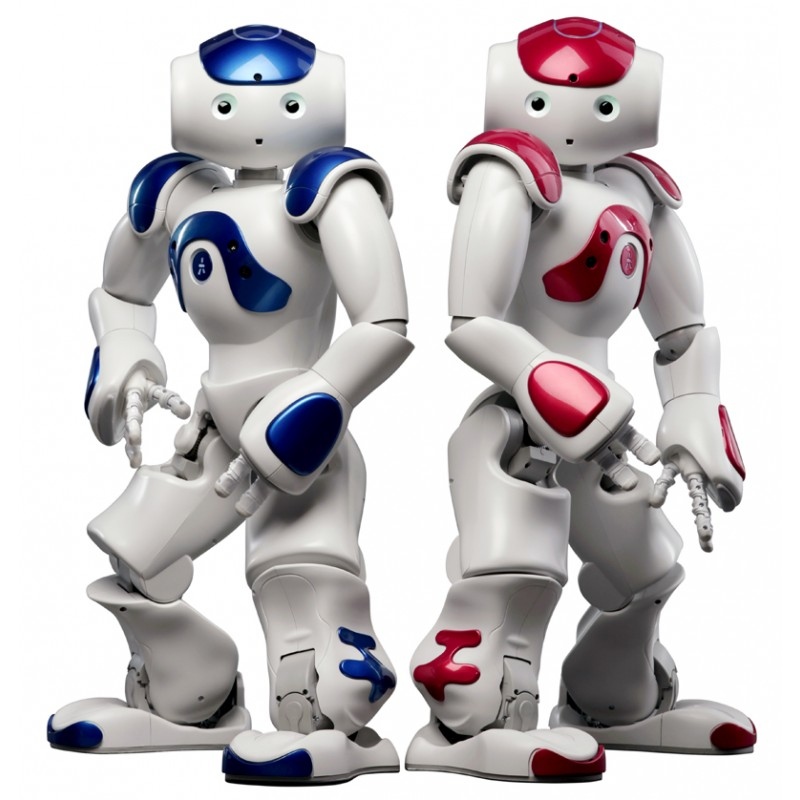
\includegraphics[width=0.55\textwidth]{chapter2/images/nao.jpg}
    \caption{หุ่นยนต์ฮิวมานอยด์นาโอะ}
    \label{fig:nao_humanoid}
\end{figure}
หุ่นยนต์ฮิวมานอยด์นาโอะ เป็นหุ่นยนต์ฮิวมานอยด์ขนาดกลาง ถูกผลิตมาจากประเทศฝรั่งเศษ พัฒนาโดยบริษัท Aldebaran Robotics เมื่อปี 2004 และในปี 2007
หุ่นยนต์ฮิวมานอยด์นาโอะได้นำไปแทนที่หุ่นยนต์สุนัขของ Sony ชื่อ Aibo ขณะถูกใช้ในรายการแข่งขัน RoboCup Standard Platform League (SPL) หุ่นยนต์นาโอะได้ถูกนำไปใช้ใน Robocup 2008 และ 2009 
หุ่นยนต์นาโอะถูกพัฒนาออกมาหลายรุ่นมีองศาอิสระตั้งแต่ 14 องศาอิสระ 21 องศาอิสระ และ 25 องศาอิสระ สำหรับเพื่องานวิจัยนั้นมีถึง 25 องศาอิสระ
โดยเพิ่มเติมมือสองข้างเอาเข้าไปเพื่อให้สามารถหยิบจับสิ่งของได้ ภายในหุ่นยนต์ถูกควบคุมด้วยระบบปฎิบัติการ NAO 2.0 (Linux-based) ตัวหุ่นยนต์มีความสูง 58 เซนติเมตร 
น้ำหนัก 4.3 กิโลกรัม ส่วนเซนเซอร์การรับรู้ต่างๆจะประกอบไปด้วย เซนเซอร์วัดมุมเอียง 3-axis gyro, 3-axis accelerometer, Ultrasound captors, ไมโครโฟน 4 ตัว ลำโพง 2 ตัว กล้อง 2 ตัว เพื่อใช้ประโยชน์ในการทำงานวิจัยต่างๆ
ตอนนี้ความสามารถของหุ่นยนต์นาโอะที่ทำได้คือ สามารถเทน้ำส้มได้ เดินขึ้นลงบันไดและทางลาดชันได้ ระหว่างการเดินนั้นสามารถวางแผนการวางเท้าได้อย่างรวดเร็ว
อีกทั้งยังสามารถที่จะเดินหลบหลีกสิ่งกีดขวางได้ด้วย

\clearpage
\subsection*{Wabot}
\begin{figure}[ht]
    \centering
    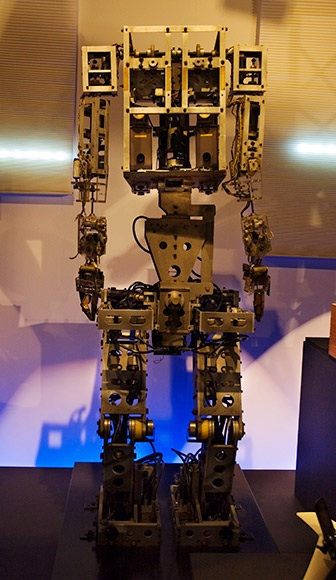
\includegraphics[width=0.45\textwidth]{chapter2/images/wabot.jpg}
    \caption{หุ่นยนต์ฮิวมานอยด์วาบอท}
    \label{fig:wabot_humanoid}
\end{figure}
หุ่นยนต์ฮิวมานอยด์มีการพัฒนาในช่วงแรกเริ่มมาตั้งแต่ปี 1973 หุ่นยนต์ฮิวมานอยด์ ตัวแรกชื่อ Wabot-1 เริ่มสร้างโดยมหาวิทยาลัย Waseda ที่ประเทศญี่ปุ่น ตัวของหุ่นยนต์มีความสูง 180 เซนติเมตร
น้ำหนัก 210 กิโลกรัม โดยหุ่นยนต์สามารถติดต่อสื่อสารกับมนุษย์ได้ด้วยภาษาญี่ปุ่น สามารถวัดระยะและทิศทางได้โดยใช้การรับรู้ผ่านทางตาและหูเทียม หุ่นยนต์ Wabot-1 นั้นสามารถเดินได้ด้วยขาของตนเองที่มีสองข้าง
สามารถหยิบและเคลื่อนย้ายวัตถุด้วยมือ ต่อมาในปี 1984 มหาวิทยาลัย Waseda ได้พัฒนาหุ่นยนต์ฮิวมานอยด์ที่ชื่อ Wabot-2 โดยหุ่นยนต์สามารถสื่อสารกับมนุษย์ได้ สามารถอ่านโน๊ตเพลงและเล่นดนตรีโดยใช้ electronic organ แบบง่ายๆได้
และในปี 1985 บริษัท Hitachi ได้สร้างหุ่นยนต์ WHL-11 ที่มีสองขาเหมือนมนุษย์ ซึ่งสามารถเดินแบบสมดุลสถิต (Static Walking) บนพื้นราบได้ด้วยความเร็ว 13 วินาทีต่อหนึ่งก้าว และสามารถเลี้ยวได้ซ้ายและขวาได้






\clearpage
\section{การออกแบบโครงสร้างของหุ่นยนต์}
\subsection{ความแตกต่างระหว่างโครงสร้างของมนุษย์กับโครงสร้างของหุ่นยนต์}

\subsubsection{ความแตกต่างขององศาเสรี}
เนื่องจากลักษณะข้อต่อของมนุษย์มีความซับซ้อนมากกว่าโครงสร้างของหุ่นยนต์
ทำให้ข้อต่อแต่ละจุดของมนุษย์นั้นสามารถหมุนได้หลายทิศทาง รวมถึงขอบเขตของการหมุนของข้อต่อในแต่จุดก็มีความแตกต่างกัน
ในการนำรูปแบบการเดินของมนุษย์ไปใช้กับหุ่นยนต์จึงต้องปรับค่ามุมที่ข้อต่อให้มีความเหมาะสมกับโครงสร้าง
และข้อจำกัดเกี่ยวกับการหมุนของข้อต่อจุดต่างๆของหุ่นยนต์ที่จะใช้ทดสอบด้วย

\subsubsection{ความแตกต่างของอัตราส่วน}
นอกจากความแตกต่างขององศาเสรี (DoF) ระหว่างมนุษย์กับหุ่นยนต์แล้ว
ความแตกต่างของอัตราส่วนระหว่างโครงสร้างแต่ละส่วนของมนุษย์กับหุ่นยนต์เป็นอีกสาเหตุหนึ่ง
ที่ต้องทำการปรับแต่งใหม่มีความเหมาะสม เนื่องจากความยาวของโครงสร้างแต่ละส่วน
รวมทั้งระยะห่างระหว่างจุดหมุนแต่ละจุดของมนุษย์กับหุ่นยนต์ที่มีความแตกต่างกัน
ดังนั้นจึงต้องกำหนดระบบพิกัดสำหรับหุ่นยนต์ฮิวมานอยด์ขึ้นมาใหม่ เพื่อใช้ในการอ้างอิงจุดหมุน
และความยาวของโครงสร้างในส่วนต่างๆ
\begin{figure}[!ht]
    \centering
    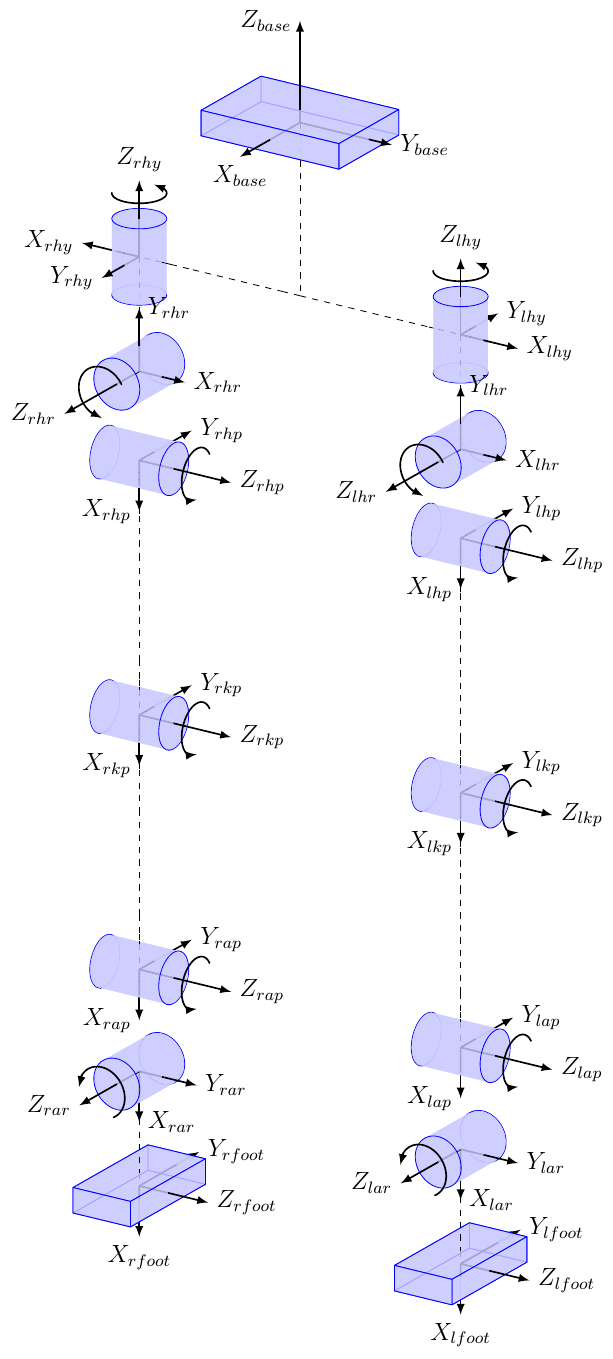
\includegraphics[width=0.40\textwidth]{chapter2/images/uthai_kinematics.png}
    \caption{ตัวอย่างตำแหน่งและการหมุนของข้อต่อของหุ่นยนต์เพื่อการอ้างอิง}
    \label{fig:robot_frame}
\end{figure}

\subsubsection{กำลังและประสิทธิภาพของมอเตอร์}
ความสามารถในการรับน้ำหนักของข้อต่อแต่ละจุดมีความแตกต่างกัน การเคลื่อนไหวของมนุษย์นั้นจะมีกล้ามเนื้อ
และเส้นเอ็นเป็นตัวออกแรงดึงส่วนต่างๆของร่างกายเพื่อทำให้เกิดการเคลื่อนไหวซึ่งจะมีความยืดหยุ่นและแรงดึงที่มีค่าสูง
สำหรับการเคลื่อนไหวของหุ่นยนต์ จะใช้การบิดแกนของเซอร์โวมอเตอร์ (Servo Motor) หรือมอเตอร์ที่ติดอยู่ที่ข้อต่อจุดต่างๆ
ทำให้ความสามารถในการรับน้ำหนัก แรงบิดและความยืดหยุ่นที่ข้อต่อขึ้นกับกำลังของมอเตอร์เป็นหลัก
การสร้างท่าทางของหุ่นยนต์จึงต้องคำนึงถึงความสามารถในการรับน้ำหนักและกำลังของเซอร์โวมอเตอร์ที่ใช้ด้วยเช่นกัน

%%%%%%%%%%%%%%%%%%%%%%%%%%%%%%%%%%%%%%%%%%%%%%%%%%%%%%%%%
%\subsection{วัสดุและการขึ้นรูปโครงสร้างของหุ่นยนต์ฮิวมานอยด์}
%\begin{figure}[ht]
%    \centering
%    
\includegraphics[width=0.40\textwidth]{chapter2/images/toedit.jpg}
%    \caption{รอแก้ไข}
%    \label{fig:toedit}
%\end{figure}

%%%%%%%%%%%%%%%%%%%%%%%%%%%%%%%%%%%%%%%%%%%%%%%%%%%%%%%%%
\subsection{อุปกรณ์ที่ใช้ในหุ่นยนต์ฮิวมานอยด์}

\subsubsection*{ตัวขับเคลื่อน}
ในการสร้างหุ่นยนต์ฮิวมานอยด์นั้นระบบการขับเคลื่อนก็ถือว่าเป็นเรื่องสำคัญ เนื่องจากว่าถ้าหากระบบขับเคลื่อนไม่สามารถทำงานได้อย่างเต็มประสิทธิภาพ
หรือหากมีการออกแบบที่ผิดพลาด จะส่งผลทำให้หุ่นยนต์ฮิวมานอยด์นั้นมีประสิทธิภาพในการทำงานลดลงตามไปด้วย ภายในงานวิจัยนี้ทางผู้จัดทำได้ใช้ตัวขับเคลื่อนเป็น
Dynamixel digital servo EX-106 ซึ่งเป็นเซอร์โวมอเตอร์ที่เหมาะสำหรับทำหุ่นยนต์โดยเฉพาะ ภายในประกอบไปด้วย มอเตอร์กระแสตรง ชุดเฟืองมอเตอร์
ไดรเวอร์คอนโทรเลอร์ สามารถเชื่อมต่อกันผ่าน BUS RS-485 มีการควบคุมแบบ PID และแรงบิดที่สูง\footnote{ Robot Actuator [http://support.robotis.com/en/product/actuator/dynamixel/ex\_series/ex-106.htm] }

\begin{figure}[!ht]
    \centering
    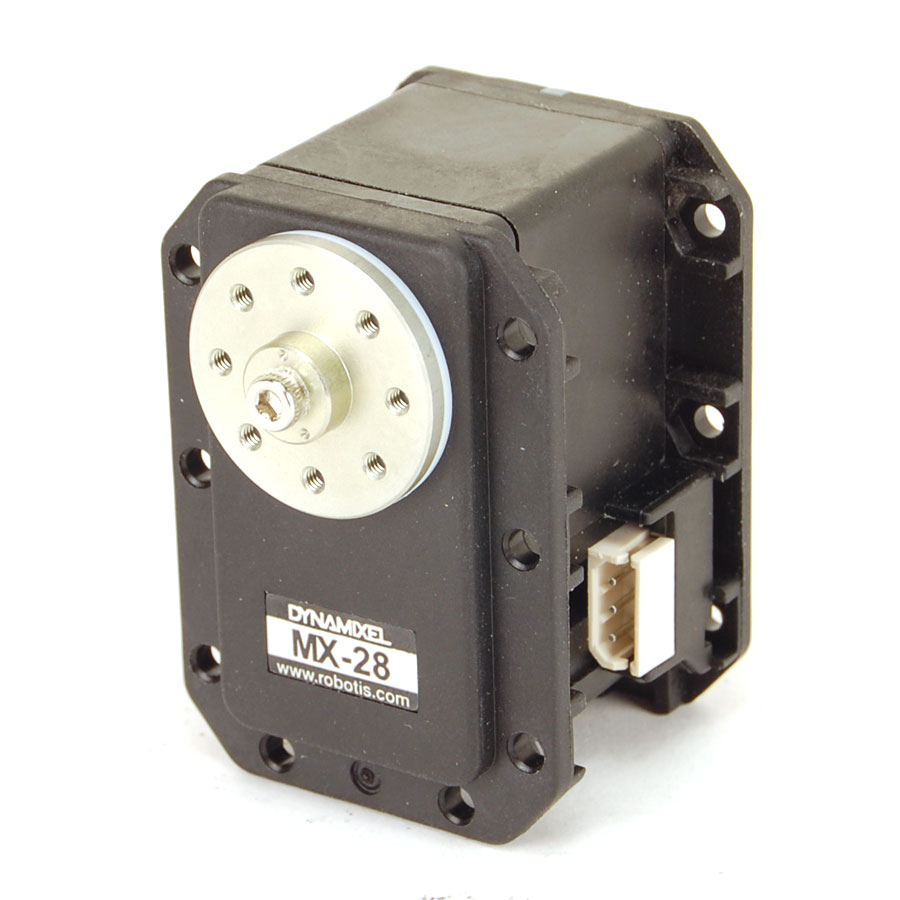
\includegraphics[width=0.3\textwidth]{chapter2/images/actuator_robot.jpg}
    \caption{ตัวขับเคลื่อนที่ใช้ในหุ่นยนต์ฮิวมานอยด์}
    \label{fig:actuator_robot}
\end{figure}

\clearpage
%%%%%%%%%%%%%%%%%%%%%%%%%%%%%%%%%%%%%%%%%%%%%%%%%%%%%%%%%
\subsubsection*{หน่วยประมวลผลควบคุม}
ในการควบคุมหุ่นยนต์ฮิวมานอยด์ให้สามารถทำกิจกรรมต่างๆได้นั้น ส่วนที่มีความสำคัญที่ขาดไปไม่ได้ คือ
หน่วยประมวลผลระบบควบคุม ถ้าหากไม่มีระบบประมวลผลควบคุมแล้ว อุปกรณ์ต่างๆ ที่ติดตั้งอยู่ภายในตัวของหุ่นยนต์ฮิวมานอยด์จะไม่สามารถติดต่อสื่อสารกันได้
ซอฟท์แวร์ของหุ่นยนต์ที่พัฒนามาทั้งหมดจะไม่สามารถใช้ได้ ทำให้หุ่นยนต์ฮิวมานอยด์ไม่สามารถทำงานในสิ่งที่ต้องการได้ 
การวางแผนระบบควบคุมที่นิยมใช้ในระบบหุ่นยนต์ฮิวมานอยด์ส่วนใหญ่ จะแบ่งออกเป็น 2 ส่วนด้วยกัน 
คือส่วนของหน่วยประมวลผลควบคุมระดับสูง และหน่วยประมวลผลควบคุมระดับต่ำ

\subsubsection*{หน่วยประมวลผลควบคุมระดับสูง (High level controller)}
หน่วยประมวลผลควบคุมระดับสูงเป็นส่วนที่ใช้ประมวลผลการทำงานที่มีความซับซ้อนของระบบเช่น
จลนศาสตร์ของหุ่นยนต์ การคำนวณหาเส้นทางการเดิน ในการคำนวณทางคณิตศาสตร์ของระบบเหล่านี้จำเป็นต้องมีการประมวลผลที่เร็ว
และมีประสิทธิภาพ ในสมัยที่มีการพัฒนาหุ่นยนต์ฮิวมานอยด์ยุคแรกเริ่มนั้น หน่วยประมวลผลควบคุมระดับสูง
จะใช้คอมพิวเตอร์เป็นตัวในการประมวลผลการคำนวณ ซึ่งคอมพิวเตอร์สมัยนั้นมีขนาดใหญ่ น้ำหนักมาก
และต้องใช้หลังงานสูง ซึ่งต่างจากปัจจุบันนี้ที่มีการพัฒนาของเทคโนโลยีที่ก้าวหน้ามากขึ้น
ทำให้คอมพิวเตอร์มีขนาดเล็กลงเทียบเท่ากับบอร์ดคอนโทรเลอร์ทั่วไป\footnote{Robot controller Robotis, Thormang, http://jp.robotis.com/index/product.php?cate\_code=111410}

\begin{figure}[!ht]
    \centering
    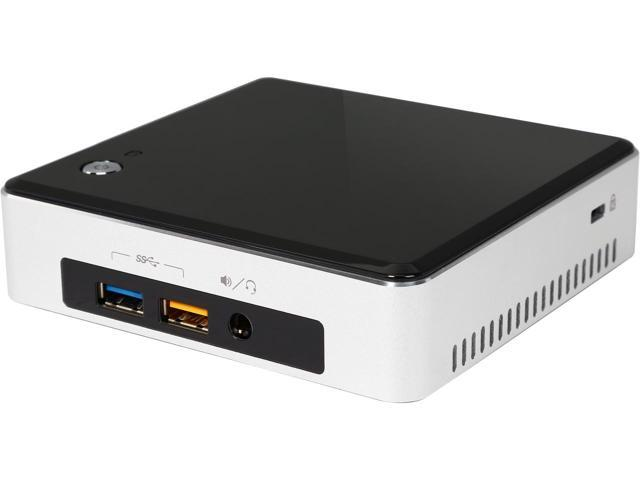
\includegraphics[width=0.3\textwidth]{chapter2/images/thormang_controller.jpg}
    \caption{ตัวประมวลผลระดับสูงของ Thormang Humanoid}
    \label{fig:thormang_controller}
\end{figure}

\subsubsection*{หน่วยประมวลผลควบคุมระดับต่ำ (Low level controller)}
หน่วยประมวลผลควบคุมระดับต่ำเป็นส่วนที่รับคำสั่งมาจากหน่วยประมวลผลควบคุมระดับสูง
มีประสิทธิภาพในการประมวลผลการคำนวณที่น้อยกว่า เนื่องจากการออกแบบสถาปัตยกรรมภายในระบบไม่เอื้ออำนวยต่อการคำนวณที่มีความซับซ้อน
แต่มีความสามารถในการประมวลผลระบบที่เป็นคาบได้อย่างแม่นยำ ในด้านการทำหุ่นยนต์ฮิวมานอยด์นั้นมักจะใช้หน่วยประมวลผลควบคุมระดับต่ำ
ในการติดต่อกับอุปกรณ์ต่างๆบนตัวของหุ่นยนต์ฮิวมานอยด์โดยตรง เช่น ตัวขับเคลื่อน เซนเซอร์รับค่า หรือไฟแสดงสถานะต่างๆของหุ่นยนต์
\begin{figure}[!ht]
    \centering
    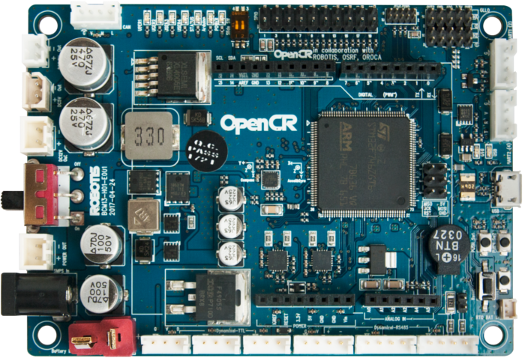
\includegraphics[width=0.30\textwidth]{chapter2/images/opencr_op3.png}
    \caption{ตัวประมวลผลระดับต่ำของ Robotis OP3 Humanoid}
    \label{fig:opencr_op3_controller}
\end{figure}

\clearpage
%%%%%%%%%%%%%%%%%%%%%%%%%%%%%%%%%%%%%%%%%%%%%%%%%%%%%%%%%
\subsubsection*{เซนเซอร์ตรวจหน้าสัมผัสที่พื้น}
เซนเซอร์ตรวจหน้าสัมผัสที่พื้นเป็นเซนเซอร์ที่ถูกติดตั้งบริเวณฝ่าเท้า เพื่อตรวจสอบการเดินของหุ่นยนต์ฮิวมานอยด์ว่าขณะนี้มีการสัมผัสของฝ่าเท้าของหุ่นยนต์กับพื้นหรือไม่
ซึ่งในงานวิจัยนี้ได้ใช้หลักการตัวตรวจจับแรงกดแบบค่าความต้านทานหรือ Force Sensing Resistor (FSR)\footnote{ [UNICON] Force sensor with UNICON [http://doc.inex.co.th/force-sensor-with-unicon/] }
ที่ใช้เทคโนโลยีฟิล์มโพลีเมอร์แบบหนาโดยที่
เซนเซอร์สามารถเปลี่ยนแรงที่มากระทำให้อยู่ในรูปของการเปลี่ยนแปลงค่าความต้านทานไฟฟ้า ตัวเซนเซอร์มีลักษณะเป็นแผ่น มีโครงสร้าง 5 ชั้น
โดยสองชั้นนอกสุดเป็นฟิล์มของโพลีเอสเตอร์ สองชั้นถัดเข้ามาเป็นฟิล์มของโลหะที่เป็นตัวนำไฟฟ้า และชั้นในสุดเป็นหมึกที่มีความไวในการตอบสนองต่อแรงภายนอกที่มากระทำ
(Pressure sensitive ink) และโครงสร้างทั้ง 5 ชั้น ถูกรวมเข้าด้วยกันด้วยวิธีลามิเนท จึงทำให้เซนเซอร์วัดแรงนี้มีลักษณะแบนมีความยืดหยุ่นสูง
ด้วยเหตุนี้จึงทำให้เซนเซอร์สามารถโค้งงอได้ง่าย แรงดันไฟฟ้าที่ตกคร่อมตัวตรวจจับจะลดลง เมื่อมีแรงกดมากระทำบนแผ่นตรวจจับ มีโครงสร้างของตัวตรวจจับแสดงในรูปที่ \ref{fig:fsr_sensor} 

\begin{figure}[!ht]
    \centering
    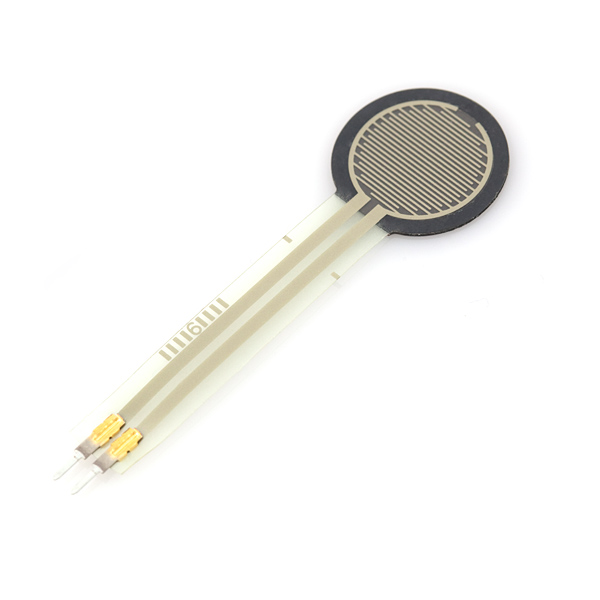
\includegraphics[width=0.15\textwidth]{chapter2/images/FSRx.jpg}
    \caption{ลักษณะโครงสร้างของตัวตรวจจับแรงกด FSR}
    \label{fig:fsr_sensor}
\end{figure}

\subsubsection*{เซนเซอร์วัดความเฉื่อย}
Inertial Measurement Unit (IMU) เป็นส่วนประกอบหลักที่ใช่ในการนำร่องเครื่องบิน ยาน-อวกาศ ดาวเทียม เรือ
ขีปนาวุธ ซึ่งในตัวของ IMU ประกอบไปด้วยสองส่วนหลักคือ Accelerometers 3 ทิศทาง ในการรับความเร่งเชิงเส้น
และ Gyroscopes 3 ทิศทาง ในการบอกความเร็วเชิงมุม เซนเซอร์ตัวนี้สามารถนำมาใช้ในการหาทิศทางการหมุนของตัวหุ่นยนต์ฮิวมานอยด์ได้

เซนเซอร์วัดความเร็ว (Gyroscope)\footnote{ Mechanic gyroscope two-degree of freedom [https://www.bosch-sensortec.com/bst/products/motion/gyroscope/overview\_gyroscopesensors] }
เป็นอุปกรณ์สำหรับการวัดความเร็ว หรือการรักษาการปรับทิศทาง ขึ้นอยู่กับหลักการของการอนุรักษ์โมเมนตัมเชิงมุม
ถ้าไม่มีการเคลื่อนที่ อัตราการเปลี่ยนแปลงมุมจะมีค่าเท่ากับศูนย์

เซนเซอร์วัดความเร่ง (Accelerometer)\footnote{ Accelerometer and Gyroscopes Sensor [https://www.maximintegrated.com/en/app-notes/index.mvp/id/5830] }
เป็นอุปกรณ์ที่ใช้วัดความเร่งเชิงเส้น โดยอาศัยการวัดแรงที่กระทำต่อน้ำหนัก
อ้างอิงที่เกิดจากแรงโน้มถ่วงโลก ซึ่งแรงโน้มถ่วงของโลกจะเป็นเวกเตอร์ชี้ไปที่แกนกลางโลกเสมอ ตามกฎของนิวตัน
\begin{figure}[!ht]
    \centering
    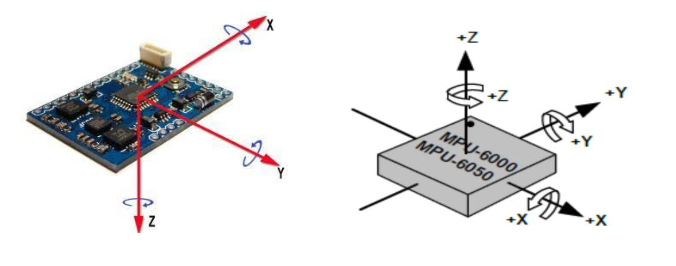
\includegraphics[width=0.5\textwidth]{chapter2/images/imu.png}
    \caption{เซนเซอร์วัดความเฉื่อย}
    \label{fig:imu_sensor}
\end{figure}

%\clearpage
%\subsection{แนวคิดการออกแบบกลไกการเดินของหุ่นยนต์ฮิวมานอยด์}
%การออกแบบหุนยนตฮิวมานอยด์ใหสามารถเดินสองขาไดเสมือนมนุษยโดยใชจํานวนองศาอิสระใหเท่ากับมนุษยนั้นพบวา
%มีขอจํากัดทางดานการออกแบบอยู่มาก เนื่องมาจากอุปกรณที่ใชในการขับเคลื่อนขอตอตางๆ มีอยูอยางจํากัด
%รวมถึงขอจํากัดทางดานตัวรับรูตัวขับของหุนยนต ดังนั้นผูจัดทําจึงออกแบบหุนยนตใหมีองศาอิสระของขอตอ ในขาหนึ่งขาง
%เทากับหกองศาอิสระ ทั้งนี้หุนยนตยังสามารถเคลื่อนที่ไดในปริภูมิ และองศาอิสระเพียงพอตอการใชงาน

\clearpage
\section{การออกแบบโปรแกรมด้วย ROS}
\subsection{ระบบที่ใช้ช่วยในการพัฒนาหุ่นยนต์}
Robot Middleware เป็นกรอบการทำงาน(framework) ที่มีความยืดหยุ่นสำหรับการพัฒนาซอฟแวร์ที่ซับซ้อนในการควบคุมของหุ่นยนต์
ตัว Robot Middleware ถูกออกแบบมาให้ใช้ในการจัดการระบบที่มีความยุ่งยาก โดยมีเครื่องมือที่ช่วยติดต่อสื่อสารระหว่างอุปกรณ์ต่างๆของหุ่นยนต์ 
Robot Middleware ส่วนใหญ่จะใช้การติดต่อสื่อสารผ่านระบบเครือข่ายเน็ตเวิร์ค ทำให้การสื่อสารในระบบพื้นฐานเป็นอิสระต่อกัน 
และสามารถติดต่อสื่อสารกันกับอุปกรณ์ที่อยู่ภายนอกผ่านเครือข่ายเดียวกันได้

ปัจจุบันมี Robot Middleware ที่ถูกพัฒนาขึ้นมาให้ใช้อยู่หลายตัวเช่น

\subsubsection*{Player Project}
\begin{figure}[ht]
    \centering
    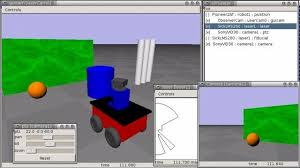
\includegraphics[width=0.45\textwidth]{chapter2/images/mdw_playerproject.jpeg}
    \caption{player project middleware}
    \label{fig:mdw_playerproject}
\end{figure}
เป็นโปรเจคที่ใช้ในการสร้างซอฟแวร์เพื่อการศึกษาวิจัยที่มีความเกี่ยวข้องกับหุ่นยนต์และระบบเซนเซอร์
ภายในประกอบไปด้วยระบบตัวกลาง และระบบจำลองการทำงานของหุ่นยนต์

\subsubsection*{YARP}
\begin{figure}[ht]
    \centering
    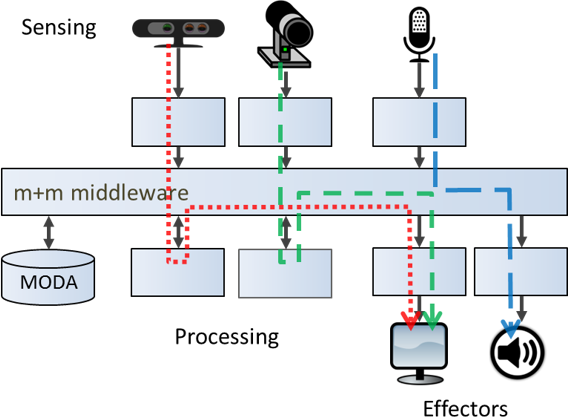
\includegraphics[width=0.45\textwidth]{chapter2/images/mdw_yarp.png}
    \caption{yarp middleware}
    \label{fig:mdw_yarp}
\end{figure}
เป็น open source ที่เขียนด้วยภาษา C++ ในการเชื่อมต่อกับเซนเซอร์ หน่วยประมวลผล และตัวขับเคลื่อนของหุ่นยนต์

\clearpage
\subsubsection*{URBI}
\begin{figure}[ht]
    \centering
    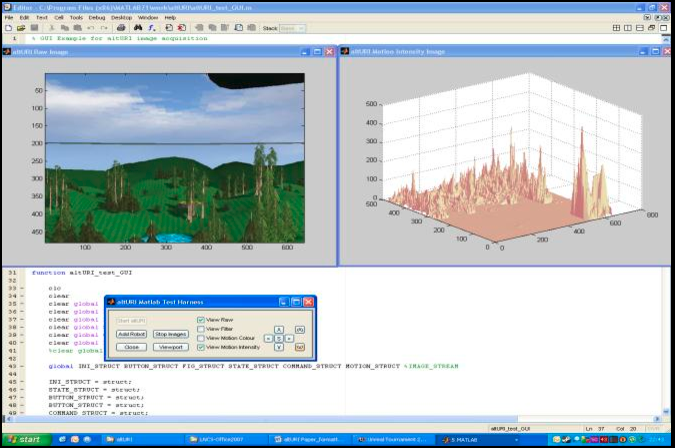
\includegraphics[width=0.45\textwidth]{chapter2/images/mdw_urbi.png}
    \caption{urbi middleware}
    \label{fig:mdw_urbi}
\end{figure}
เป็น open source สำหรับพัฒนาแอพพลิเคชั่นที่เกี่ยวข้องกับหุ่นยนต์หรือระบบที่มีความซับซ้อน ใช้ภาษาพื้นฐานเป็นภาษา C++ ติดต่อสื่อสารได้ภายในเครือข่ายเดียวกันเท่านั้น (Local Network)

\subsubsection*{MIRO}
\begin{figure}[ht]
    \centering
    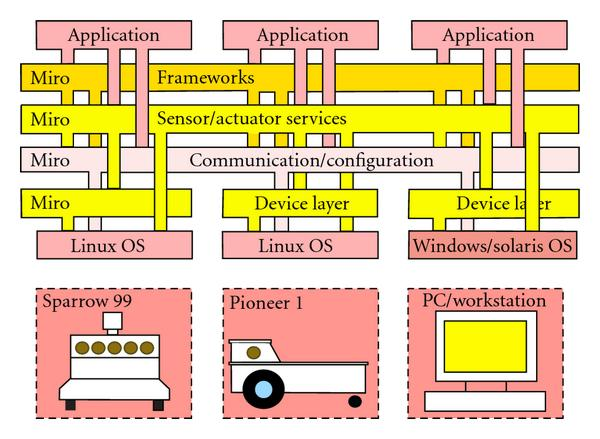
\includegraphics[width=0.45\textwidth]{chapter2/images/mdw_miro.jpeg}
    \caption{miro middleware}
    \label{fig:mdw_miro}
\end{figure}
เป็นกรอบการทำงานของหุ่นยนต์ที่เคลื่อนที่ได้โดยเขียนในลักษณะเป็น OOP

\subsubsection*{OpenRDK}
\begin{figure}[ht]
    \centering
    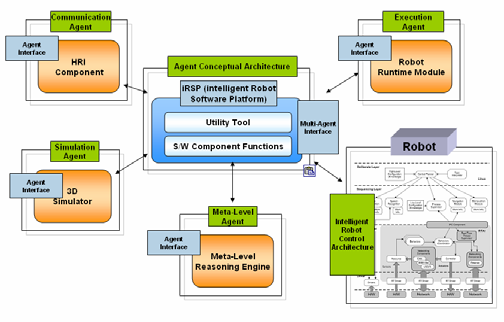
\includegraphics[width=0.45\textwidth]{chapter2/images/mdw_openrdk.png}
    \caption{openrdk middleware}
    \label{fig:mdw_openrdk}
\end{figure}
เป็น open source สำหรับพัฒนาระบบที่มีความเป็นอิสระต่อกัน (Modules) สามารถใช้ช่องทางการติดต่อสื่อสารและหน่วยความจำร่วมกันได้

\subsubsection*{ROS}
Robot Operating System หรือ ROS ถูกพัฒนาโดยบริษัท Willow Garage, แตเดิมแลวเคาพัฒนาเพื่อใช
งานกับหุนยนต PR2 ในป 2007 ซึ่งพัฒนาเปน open source framework สําหรับนักพัฒนาซอฟแวรที่เกี่ยวของ
กับหุนยนต มีความสามารถในการทํางานแบบ parallel บนคอมพิวเตอรหลายๆเครื่องได สามารถทํางานไดหลาย
OS นอกจากนี้ยังมีคลังที่คอยเก็บซอฟแวรตางๆไวเปน libraries อีกดวย การใช ROS
จะชวยทําใหเราสามารถพัฒนาหุนยนตไดอยางรวดเร็วมากขึ้น ประหยัดเวลา ประหยัดทรัพยากร

\begin{figure}[ht]
    \centering
    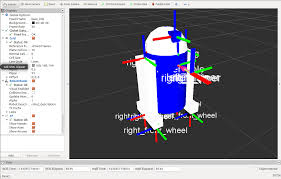
\includegraphics[width=0.5\textwidth]{chapter2/images/mdw_ros.jpeg}
    \caption{ROS middleware Rviz}
    \label{fig:mdw_ros}
\end{figure}
\begin{figure}[ht]
    \centering
    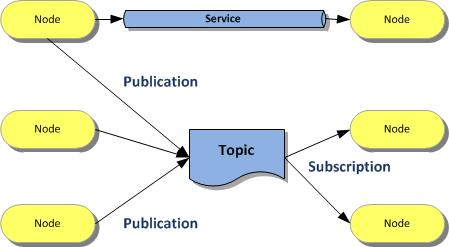
\includegraphics[width=0.5\textwidth]{chapter2/images/mdw_ros2.jpeg}
    \caption{ROS algitecture}
    \label{fig:mdw_ros2}
\end{figure}
\begin{figure}[ht]
    \centering
    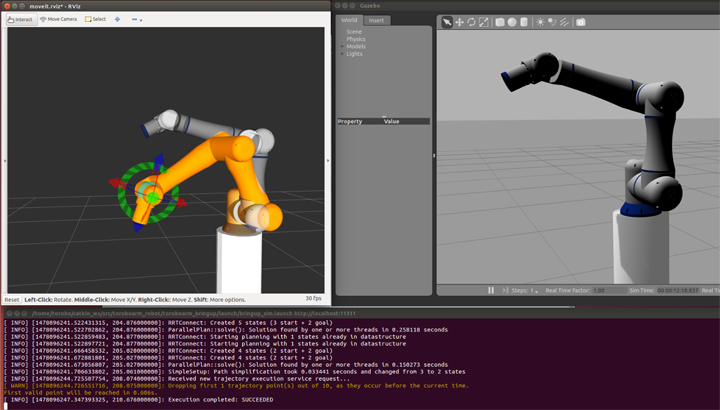
\includegraphics[width=0.5\textwidth]{chapter2/images/mdw_ros3.jpeg}
    \caption{ROS Moveit}
    \label{fig:mdw_ros3}
\end{figure}

\clearpage
\subsection{ระบบที่ใช้ในการจำลองการทำงานของหุ่นยนต์}
โปรแกรมจำลองการทำงานของหุ่นยนต์นั้นเป็นเครื่องมือที่สำคัญสำหรับนักหุ่นยนต์ การใช้โปรแกรมจำลองนั้นจะช่วยเพิ่มประสิทธิภาพในการทำงานหลายอย่าง
เช่น ให้รู้ว่าหุ่นยนต์ที่ออกแบบนั้นสามารถทำงานได้อย่างที่ต้องการหรือไม่ กระบวนการคิดถูกต้องหรือไม่
โปรแกรมจำลองระบบส่วนใหญ่จะคำนวณพลวัตของหุ่นยนต์โดยใช้เครื่องมือคำนวณ open dynamics engine (ODE)

\subsubsection*{USARSim}
\begin{figure}[ht]
	\centering
	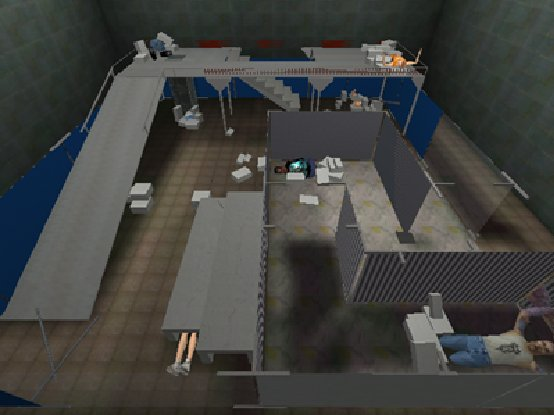
\includegraphics[width=0.5\textwidth]{chapter2/images/sim_USARSim.jpg}
    \caption{ผลลัพธ์จากการใช้โปรแกรม USARSim}
    \label{fig:sim_USARSim}
\end{figure}
USARSim เป็นโอเพนซอร์ซและเหมาะสำหรับทำหุ่นยนต์ประเภทกู้ภัยในซากเมือง โดยมีฐานการพัฒนามาจาก 
Unreal Tournament game engine ภายในโปรแกรมมีเครื่องมือสำหรับการทำงานวิจัย มีเซนเซอร์ของหุ่นยนต์ที่หลากหลาย 
เช่น เซนเซอร์รับภาพ หรือเซนเซอร์ตรวจความเคลื่อนไหว

\subsubsection*{MuRoSimF}
\begin{figure}[ht]
    \centering
    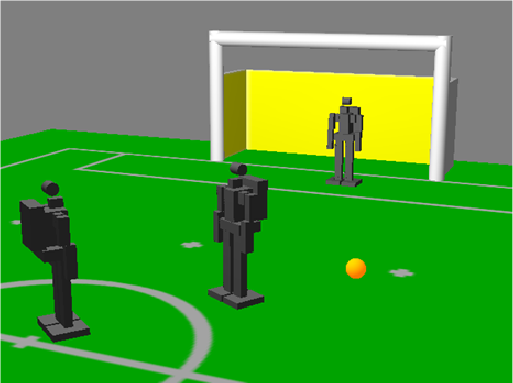
\includegraphics[width=0.5\textwidth]{chapter2/images/sim_MuRoSimF.png}
    \caption{ผลลัพธ์จากการใช้โปรแกรม MuRoSimF}
    \label{fig:sim_MuRoSimF}
\end{figure}
MuRoSimF ย่อมาจากคำว่า Multi-Robot Simulation Framework เป็นเครื่องมือที่ช่วยทำระบบจำลองจาก
Darmstadt University โปรแกรมระบบจำลองนี้มีการใช้งานที่ง่าย เหมาะสำหรับหุ่นยนต์หลายประเภท เช่น
หุ่นยนต์เคลื่อนที่ด้วยล้อ หุ่นยนต์สองขา หรือหุ่นยนต์หลายขา สามารถคำนวณพลวัตร และการขัดกันของก้านต่อต่างๆได้

\subsubsection*{Gazebo}
\begin{figure}[ht]
    \centering
    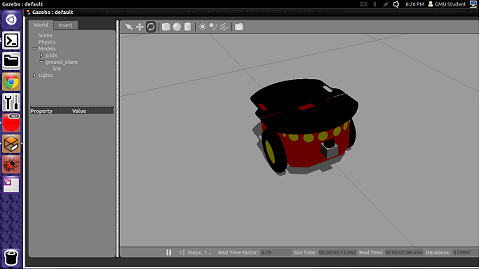
\includegraphics[width=0.5\textwidth]{chapter2/images/sim_gazebo1.png}
    \caption{Mobile robot with gazebo}
    \label{fig:sim_gazebo1}
\end{figure}
\begin{figure}[ht]
    \centering
    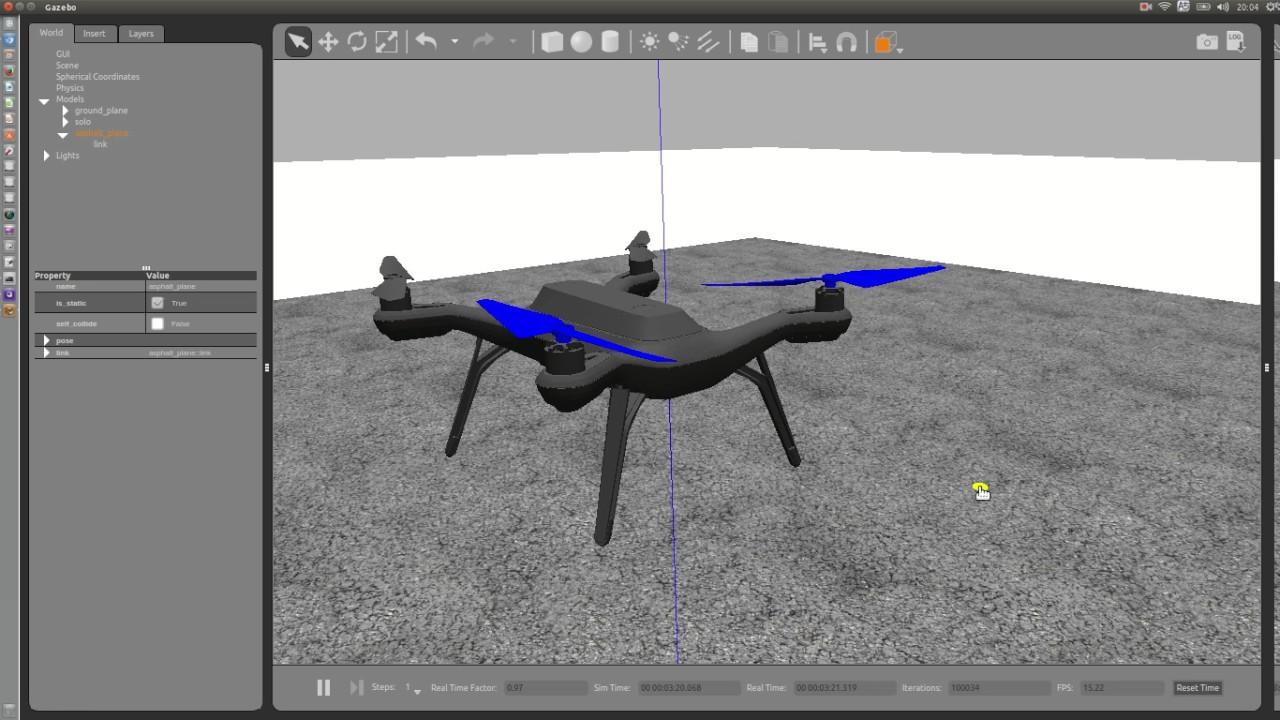
\includegraphics[width=0.5\textwidth]{chapter2/images/sim_gazebo2.jpg}
    \caption{Quadrotor with gazebo}
    \label{fig:sim_gazebo2}
\end{figure}
Gazebo เป็นโปรแกรมจำลองการทำงานของหุ่นยนต์ ที่มีความสามารถในการคำนวณการเดินและการเคลื่อนที่ของหุ่นยนต์ที่สลับซับซ้อนได้ สามารถเห็นภาพกราฟฟิคของหุ่นยนต์ขณะทำงาน โดยผู้ใช้สามารถกำหนดค่าตัวแปรทางฟิสิกส์ต่าง ๆได้ เช่นน้ำหนัก ค่าความเฉื่อย แรงเสียดทานของข้อต่อ ทำให้การออกแบบหุ่นยนต์หรือทดลองโปรแกรมได้เหมือนกับโลกจริง มีแสง มีเงา และ พื้นผิวของวัตถุ และที่พิเศษคือสามารถสังเคราะห์ค่าของเซนเซอร์ เซนเซอร์พร้อมสัญญาณรบกวน ค่าระยะทาง แรงบิด และอื่นๆ คำนวณพลศาสตร์ของหุ่นยนต์โดยใช้ตัวคำนวณทางฟิสิกส์เป็น Bullet หรือ Simbody ในการจำลองหุ่นยนต์ในโปรแกรมนี้จำเป็นต้องได้รับไฟล์ข้อมูลของหุ่นยนต์มาก่อนซึ่งอยู่ในรูปแบบของ URDF ซึ่ง URDF คือ ประเภทของไฟล์ที่บ่งบอกถึงความสัมพันธ์ของข้อต่อและก้านต่อแต่ละชิ้นในตัวหุ่นยนต์ มีความสามารถในการอธิบายถึงกลศาสตร์และการเคลื่อนที่ของหุ่นยนต์ รวมถึงตรวจสอบการขัดกันของก้านต่อในหุ่นยนต์ได้ ภายในไฟล์นี้จะประกอบไปด้วย

\paragraph*{Link :}
คือก้านต่อของหุ่นยนต์ซึ่งภายในจะสามารถบอกขนาด รูปร่าง สี และสามารถ import 3d mesh เข้ามาได้ด้วย อีกทั้งยังสามารถใส่รายละเอียดของการเคลื่อนที่ ของก้านต่อได้เช่น inertial matrix และ collision properties

\paragraph*{Joint :}
คือข้อต่อของหุ่นยนต์สามารถกำหนดกลศาสตร์และการเคลื่อนที่ได้เช่น Joint limits ของข้อต่อที่กำลังหมุนและความเร็วการหมุน ซึ่งข้อต่อมีหลายแบบที่สามารถกำหนดได้เช่น ข้อต่อแบบหมุน, ข้อต่อแบบเลื่อน, ข้อต้อต่อแบบยึดติด, ข้อต่อแบบต่อเนื่อง

%%%%%%%%%%%%%%%%%%%%%%%%%%%%%%%%%%%%%%%%%%%%%%%%%%%%%%%%%%%%%%%%%%%%
\clearpage
\subsection{Robot Operating System}
Robot Operating System หรือ ROS ถูกพัฒนาโดยบริษัท Willow Garage, แต่เดิมแล้วเค้าพัฒนาเพื่อใช้งานกับหุ่นยนต์ PR2 ในปี 2007
ซึ่งพัฒนาเป็น open source framework สำหรับนักพัฒนาซอฟแวร์ที่เกี่ยวข้องกับหุ่นยนต์ มีความสามารถในการทำงานแบบ parallel
บนคอมพิวเตอร์หลายๆเครื่องได้ สามารถทำงานได้หลาย OS แต่ที่ซัพพอร์ทจริงๆคือ Ubuntu และ Debian นอกจากนี้ยังมีคลังที่คอยเก็บซอฟแวร์ต่างๆไว้เป็น
libraries อีกด้วย การใช้ ROS จะช่วยทำให้เราสามารถพัฒนาหุ่นยนต์ได้อย่างรวดเร็วมากขึ้น ประหยัดเวลา ประหยัดทรัพยากร
ในส่วนนี้จะกล่าวถึง ROS คร่าวๆ

\subsubsection*{Nodes}
Node เป็นเหมือนหน่วยประมวลผลในระบบ ROS, Node สามารถที่จะส่งข้อมูลหาโหนดอื่นๆได้ ผ่าน Topics หรือ Services
ในทางปฏิบัติแล้วโหนดเป็นตัวประมวลผลย่อยๆ ที่คอยทำหน้าที่เฉพาะ ยกตัวอย่างเช่น โหนดตัวแรกเชื่อมต่อกับกล้อง
เพื่อที่จะนำภาพจากกล้องออกมา โหนดตัวที่สองใช้ในการหาลูกบอลที่อยู่ในภาพที่ได้มาจากโหนดตัวแรก และโหนดตัวที่สามใช้ในการคำนวณหาตำแหน่งของลูกบอลที่อยู่บนโลกจริงๆ
จากตำแหน่งของลูกบอลที่ได้มาจากโหนดที่สอง ดังนั้นจะเห็นว่าแต่ละโหนดจะทำงานเฉพาะของตัวเอง ซึ่งสามารถนำมารวมกันได้ การเขียนเป็นแบบโหนดจะช่วยทำให้เราสามารถที่จะนำโปรแกรมกลับมา
แก้ไขปรับปรุงให้ใช้ใหม่ได้ง่าย ในกรณีที่จะนำไปทำงานอย่างอื่น ยกตัวอย่างเช่น โหนดที่เอาภาพจากกล้องออกมา อาจจะมีโหนดอีกตัว ทำหน้าที่ในการหาโกลด์เป้าหมาย และหาทิศทางการเคลื่อนที่ของหุ่นยนต์ได้
ดังนั้นการพัฒนาโหนดเป็นส่วนย่อยๆเล็กๆ ก็เพื่อที่จะทำให้การแก้ไขหรือปรับปรุงได้ง่าย
\begin{figure}[ht]
	\centering	    
	\begin{tikzpicture}[shorten > = 1pt,scale=0.9, transform shape]
		% Place nodes
		\node [node] (image_provider) {image\_provider};
		\node [topic, below of=image_provider] (/image) {/image\\sensor\_msgs/Image.msg};
		\node [node, below left of=/image] (line_detection) {line\_detection};
		\node [node, below right of=/image] (stop_detection) {stop\_detection};
		\node [topic, below of=line_detection,xshift=-0.5cm] (/line) {/line\\example\_msgs/Line.msg};
		\node [topic, below of=stop_detection,xshift=0.5cm] (/stop) {/stop\\example\_msgs/Stop.msg};
		\node [node, below of=/image, yshift=-3.0cm] (navigation) {navigation};
		\node [topic, below of=navigation] (/cmd_vel) {/cmd\_vel\\geometry\_msgs/Twist.msg};
		\node [node, below of=/cmd_vel,yshift=1cm] (robot_control) {robot\_control};
		% % Draw edges
		\path [line] (image_provider) -- (/image);
		\path [line] (/image) -- (line_detection);
		\path [line] (/image) -- (stop_detection);
		\path [line] (line_detection) -- (/line);
		\path [line] (stop_detection) -- (/stop);
		\path [line] (/line) -- (navigation);
		\path [line] (/stop) -- (navigation);
		\path [line] (navigation) -- (/cmd_vel);
		\path [line] (/cmd_vel) -- (robot_control);
	\end{tikzpicture}
	\caption{ตัวอย่างสถาปัตยกรรมของ ROS}
	\label{fig:ros_architecture}
\end{figure}

จากตัวอย่างสถาปัตยกรรมของ ROS ดังรูปที่ \ref{fig:ros_architecture} นั้นสามารถอธิบายได้ว่า หุ่นยนต์เคลื่อนที่ด้วยล้อมีภารกิจคือ
เคลื่อนที่ตามเส้นไปเรื่อยๆจนกว่าจะเจอเครื่องหมายหยุด Node คือตัวที่แสดงด้วยรูปวงรี ข้างในเป็นชื่อโหนด ส่วน Topic จะแสดงด้วยรูปสี่เหลี่ยม
ซึ่งข้างในเป็นชื่อของ Topic และชนิดของ Message ที่ใช้ในการส่งข้อมูล, มาดูกันก่อนอื่น ภาพถูกส่งมาจากกล้อง และก็มีโหนดสองตัวในการดูเส้น และเครื่องหมายหยุด
จากภาพที่ได้มา เมื่อโหนดได้ข้อมูลแล้วก็นำมาประมวลผลการเดินของหุ่นยนต์โดยส่งไปยัง node navigation และโหนดนี้ก็จะทำหน้าที่คำนวณความเร็วและทิศทางของหุ่นยนต์
ส่งไปยัง node robot\_control ซึ่งเป็นตัวสั่งการมอเตอร์ของหุ่นยนต์อีกทีนึง
\begin{table}[ht]
	\begin{subtable}[h]{0.40\textwidth}
		\centering
		\begin{tabular}{| p{4cm}| p{1.5cm} |}
			\hline 
			\multicolumn{2}{|c|}{Twist.msg} \\
			\hline
			geometry\_msgs/Vector3 & linear  \\
			geometry\_msgs/Vector3 & angular \\
			\hline  
		\end{tabular}
		\caption{Message Twist}
		\label{tab:message_twist}
	\end{subtable}
	\hfill
	\begin{subtable}[h]{0.40\textwidth}
		\centering
		\begin{tabular}{| p{1.5cm}| p{2.5cm} |}
			\hline 
			\multicolumn{2}{|c|}{Stop.msg} \\
			\hline
			uint8   & RED = 0   \\
			uint8   & GREEN = 1 \\
			uint8   & color     \\
			float32 & distance  \\
			\hline  
		\end{tabular}
		\caption{Message Stop}
		\label{tab:message_stop}
	\end{subtable}
	\caption{ตัวอย่างชื่อและข้อมูลของ Message}
	\label{tab:message_example}
\end{table}

ตัวอย่างของ Message สองอันนี้ Twist message (รูปที่ \ref{tab:message_twist}) คือ message ที่เอาไว้บอกความเร็วเชิงเส้น และความเร็วเชิงมุม
ซึ่ง ROS มี message ชนิดนี้ให้อยู่แล้ว ส่วน Stop message (รูปที่ \ref{tab:message_stop}) คือ message ที่เอาไว้บอกระยะทางและสีของป้าย Stop
ซึ่ง message นี้ถูกสร้างขึ้นมาใหม่เพื่อใช้กับงานนี้โดยเฉพาะ

\subsubsection*{Topics and Messages}
Messages เป็นตัวหลักสำคัญในการติดต่อสื่อสารกันระหว่างโหนดใน ROS โดยที่ message จะถูกส่งผ่านไปยัง topic เสมอ
แต่ละ Node สามารถที่จะ subscribe หรือ publish ไปกี่ topic ก็ได้ การเชื่อมต่อกันระหว่าง Node นั้นสามารถส่งอยู่ภายในเครื่องคอมพิวเตอร์เครื่องเดียวกัน
หรือเครื่องอื่นได้ที่อยู่ใน network เดียวกัน โดยจะติดต่อสื่อสารโดยใช้ TCP/IP การใช้คอมพิวเตอร์หลายเครื่องก็จะช่วยให้การประมวลผลมีประสิทธิภาพมากยิ่งขึ้น
นอกจากนั้นยังสามารถที่จะแบ่งหน้าที่การทำงานออกจากกันได้ เราสามารถที่จะสร้าง Topic หรือ Message ขึ้นมาเองได้
หากต้องการใช้งานที่เฉพาะทาง

\subsubsection*{roscore}
roscore เป็นส่วนกลางในการรันระบบทั้งหมด เราจะเรียกกันว่า rosmaster ซึ่งมีหน้าที่ในการจัดการ
topics ทั้งหมด ที่ต้องการจะเชื่อมต่อกันไม่ว่าจะเป็นการ publish หรือ subscribe แต่ rosmaster
จะเป็นแค่ตัวจัดการเท่านั้นไม่ได้เป็นตัวที่เก็บ message ต่างๆที่ส่งไปมา ดังนั้น rosmaster จะไม่ทำให้เกิดคอขวด เวลารันระบบ
ในกระบวนการก็คือ subscribe node จะถาม rosmaster ว่ามี topic ที่ตัวเองต้องการรับข้อมูลไหม
ส่วนตัว master ที่เก็บค่า topic message เอาไว้ ก็จะส่งไปยัง subscribe node ถ้าหากมีชื่อตรงตามที่ร้องขอมา
และ rosmaster ก็จะจำไว้ว่ามี node ไหนเชื่อมต่อกับ node ไหนบ้าง

rosparameter server เป็นตัวในการเก็บค่าต่างๆที่เป็น global key-value ซึ่งช่วยให้ node ทุกตัวสามารถใช้ข้อมูลตัวเดียวกันได้
สามารถปรับเปลี่ยนระหว่างการทำงานอยู่ได้ โดยใช้ rqt plugin ซึ่งจะกล่าวในส่วนถัดไป

roslog เป็นตัวที่ใช้สำหรับ logging ข้อมูลต่างๆ ซึ่งจะถูก publish ออกมาทาง topic /rosout ซึ่งเราสามารถที่จะเขียนโปรแกรม
subscribe จากตัว topic นี้ไปเก็บเป็นไฟล์ได้

%%%%%%%%%%%%%%%%%%%%%%%%%%%%%%%%%%%%%%%%%%%%%%%%%%%%%%%
\subsubsection*{Services}
Services หรืออีกชื่อนึงคือ remote procedure calls (RPC) ความหมายคือเป็นการส่ง messages แบบที่ไม่ได้เจาะจงว่าจะส่งไปที่ไหน
เมื่อเราเรียก service แล้วระบบจะรอจนกว่าจะมีการตอบกลับ เราจะเรียกกระบวนการนี้ว่า request และ response message
Node ที่คอยทำงานเมื่อมีการเรียกใช้ service จะเรียกว่า service server และ node ที่เรียก service จะเรียกว่า service client
การใช้งาน service เหมาะสำหรับงานที่ต้องการความรวดเร็ว (fast task) แต่ไม่ควรใช้กับระบบที่ต้องใช้เวลานาน
เพราะระบบจะหยุดไม่ยอมทำต่อ ต้องรอให้ service ทำงานเสร็จก่อน สำหรับงานที่ต้องใช้เวลาในการคำนวณนานจะไปใช้ action
แทน จะกล่าวในส่วนถัดไป 


\subsubsection*{Actions}
Actions จะใช้กับการทำงาน การประมวลผลที่ต้องใช้เวลานานในการทำงาน หรือที่เรียกว่า asynchronously task
ในแต่ละ action จะมี message อยู่ 3 ชนิด คือ goal, feedback และ result Node ที่เป็นตัวรันและรอให้ node อื่นมากเรียก
จะเรียกว่า action server ส่วน node ที่เรียกการทำงาน action จะเรียกว่า action client การใช้งาน action จะเริ่มจาก
action client จะส่ง message goal ไปยัง action server แล้ว action server จะพยายามทำตาม goal ที่ได้รับมา ในระหว่างที่
action client ก็จะทำงานของตัวเองต่อไป แต่จะได้รับ feedback จาก action server อยู่ตลอดเวลา และเมื่อถึง goal ที่กำหนดแล้ว
server จะแจ้งมาทาง result message

\subsubsection*{Code Organization}
ส่วนที่เล็กที่สุดของการจัดการซอฟแวร์ใน ROS ก็คือ package ภายใน package จะมีไฟล์ที่ชื่อว่า package.xml
ซึ่งไฟล์นี้จะทำหน้าที่ในการ อธิบายและบอกข้อมูลต่างๆที่เกี่ยวกับ package นี้ ยกตัวอย่างเช่น
ชื่อของ package, ชื่อของผู้เขียน, ลิขสิทธ์ และ dependencies ที่ต้องใช้กับ package นี้
นอกจากนี้ยังสามารถใส่ข้อมูลอื่นๆเกี่ยวกับ node ลงไปเพิ่มเติมได้

\begin{figure}[ht]
    \centering
    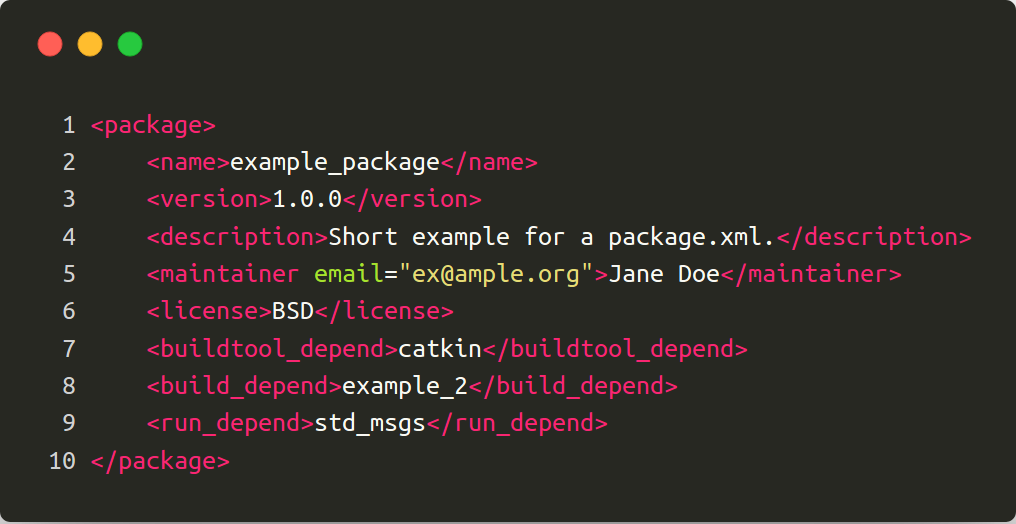
\includegraphics[width=0.8\textwidth]{chapter2/images/example_packagexml.png}
	\caption{ตัวอย่างไฟล์ package.xml}
    \label{fig:example_packagexml}
\end{figure}

แต่ละ tags ใช้ในการบอกข้อมูลของ package นี้ ใครเป็นเจ้าของ ใครเป็นคนเขียน รวมไปถึง dependencies
ที่จำเป็นต้องใช้ของ package นี้ด้วย ดังรูปที่ \ref{fig:example_packagexml} 

%%%%%%%%%%%%%%%%%%%%%%%%%%%%%%%%%%%%%%%%%%%%%%%%%%%%%%%
\clearpage
\subsubsection*{Code Distribution}
การที่จะนำ Nodes กลับมาใช้ใหม่หรือเอาออกมาแชร์ได้นั้น จะต้องมีการทำเอกสารของ Packages นั้นๆด้วย
โดยปกติแล้วจะถูกนำไปเก็บไว้ที่ GitHub และ package dependencies จะบอกไว้ในไฟล์ package.xml
เรียบร้อยแล้ว เพื่อให้ง่ายต่อการนำไปติดตั้ง หากผู้ที่นำไปใช้พัฒนาต่อหรือแก้ไขข้อผิดพลาดก็สามารถที่จะช่วยกันได้
โดยการ Pull request หรือ Report issues ได้

%%%%%%%%%%%%%%%%%%%%%%%%%%%%%%%%%%%%%%%%%%%%%%%%%%%%%%%
\subsubsection*{ROS Packages ที่ใช้ในงานวิจัย}
Package คือพื้นฐานของ ROS, แอพพลิเคชั่นทั้งหมดใน ROS จะพัฒนาโดยมี package เป็นรากฐาน ใน package นั้นจะเก็บพวกไฟล์
configuration ไปจนถึงไฟล์ launch ที่สามารถไปรัน package หรือ node อื่นๆได้ ตอนนี้ ROS มี packages มากกว่า 5000 packages แล้ว

Metapackage เป็นการรวมกันของ packages ที่ทำหน้าที่คล้ายๆกันหลายๆตัวมารวมไว้ที่เดียวเพื่อจะได้ใช้งานง่าย
ตัวอย่าง Navigation metapackage ประกอบไปด้วย 10 packages เช่น [AMCL(partical filter), DWA, EKF(extended kalman filter) 
และ map\_server] ซึ่งหากติดตั้ง metapackage ตัวนี้ก็จะได้มาหมดเลย

ในส่วนนี้จะอธิบายคร่าวๆถึง ROS standard packages ที่จะเอามาใช้ในงานวิจัยครั้งนี้

\paragraph*{rosbag}
rosbag เป็นแพกเกจที่สามารถบันทึก message ที่ส่งหากันในระหว่างที่ ROS กำลังทำงานได้
ไฟล์ที่บันทึกจะเรียกว่า rosbag ประโยชน์ของมันคือเราสามารถเอาเข้ามาใช้ในการตรวจสอบ
หรือนำมาเล่นซ้ำได้ อีกทั้งยังง่ายต่อการค้นหาข้อผิดพลาดอีกด้วย

\paragraph*{tf2}
tf2 เป็นแพกเกจที่สามารถติดตามการเปลี่ยนแปลงของ Coordinate frame เราสามารถใช้ในการหาความสัมพันธ์ระหว่าง
frame ได้ ยกตัวอย่างเช่นหากเราต้องการหาตำแหน่งของ foot เทียบกับ pelvis ก็สามารถใช้ tf2 หาได้

\paragraph*{robot\_state\_publisher}
robot\_state\_publisher แพกเกจที่ subscribe JointState message เพื่อที่จะนำตำแหน่งของของข้อต่อ
และแปลงให้อยู่ในรูปข้อมูลของ tf2, tf2 สามารถเรียกจาก Node ใดๆก็ได้เพื่อที่จะหา Coordinate frame ที่ต้องการได้

\paragraph*{URDF}
Unified Robot Description Format (URDF) เป็นไฟล์ XML ที่เอาไว้อธิบายลักษณะของหุ่นยนต์
ใน ROS มีแพกเกจที่ใช้สำหรับการอ่านไฟล์ คือ urdf\_parser แต่ไฟล์นี้ก็มีการใช้งานโดย tf2 เช่นกัน

\paragraph*{xacro}
xacro เป็นไฟล์ XML เช่นเดียวกับ URDF โดยไฟล์ xacro นี้มีประโยชน์มากในการใช้งานใน ROS เพราะว่าทำให้การเขียนไฟล์
URDF ง่ายขึ้น เพราะสามารถทำเป็นมาโครได้ สามารถปรับแต่งค่าตัวแปรต่างๆได้ง่ายขึ้น

%%%%%%%%%%%%%%%%%%%%%%%%%%%%%%%%%%%%%%%%%%%%%%%%%%%%%%%
\clearpage
\subsubsection*{Visualization}
จุดแข็งสำคัญของ ROS อีกอย่างก็คือ มีเครื่องมือที่ช่วยในการแสดงผล Visualization ได้ นอกเหนือจากระบบ
publisher-subscriber การใช้ Visualization tools นี้จะช่วยให้การทำงานง่ายขึ้นและประหยัดเวลามากขึ้น
ในการนำข้อมูลต่างๆจากหุ่นยนต์ออกมาแสดงผล เพราะว่า Visualization tools นี้สามารถที่จะ subscribe
จาก topic ที่มีการใช้งานอยู่แล้วมาแสดงผลได้ทันที ใน ROS มีเครื่องมือสำคัญอยู่ 2 ตัวที่ใช้สำหรับการ Visualization
ซึ่งสามารถที่จะปรับแต่งให้กลายเป็นเวอร์ชั่นของเราเองได้

\paragraph*{rqt}
rqt เป็น UI ที่มีฐานมาจาก QT ซึ่งมาพร้อมกับการเชื่อมต่อ ROS เป็นส่วนเสริมในรูปแบบของ QtWidget
เราสามารถที่จะแสดงผลหลายๆ widgets ได้ภายในเวลาเดียวกัน สามารถที่จะย่อขยาย เปลี่ยนตำแหน่ง
ลากวางได้ การเชื่อมต่อกับ ROS นั้นสามารถนำการแสดงผลแบบ 2D ไปแสดงได้ดังรูปที่ \ref{fig:ros_gui_example}
เป็นการแสดงภาพของกราฟที่ได้รับข้อมูลมาจาก topic หลายๆตัว และสามารถที่จะปรับแต่งค่าและ publish
ออกไปได้ด้วยการเขียนโปรแกรมเข้าไป ซึ่งจะเป็นประโยชน์อย่างมากเวลาที่ใช้ในการปรับจูนพารามิเตอร์ต่างๆ
เพราะว่าเราสามารถที่จะเปลี่ยนค่าได้ทันที ไม่ต้องรันโปรแกรมใหม่ ในรูปที่ \ref{fig:ros_gui_example}
เป็นการนำ rqt มาเขียนเป็น GUI ให้ผู้ใช้สามารถใช้งานได้ง่ายและสามารถที่จะปรับแต่งพารามิเตอร์ต่างๆได้เรียลไทม์

\begin{figure}[ht]
    \centering
    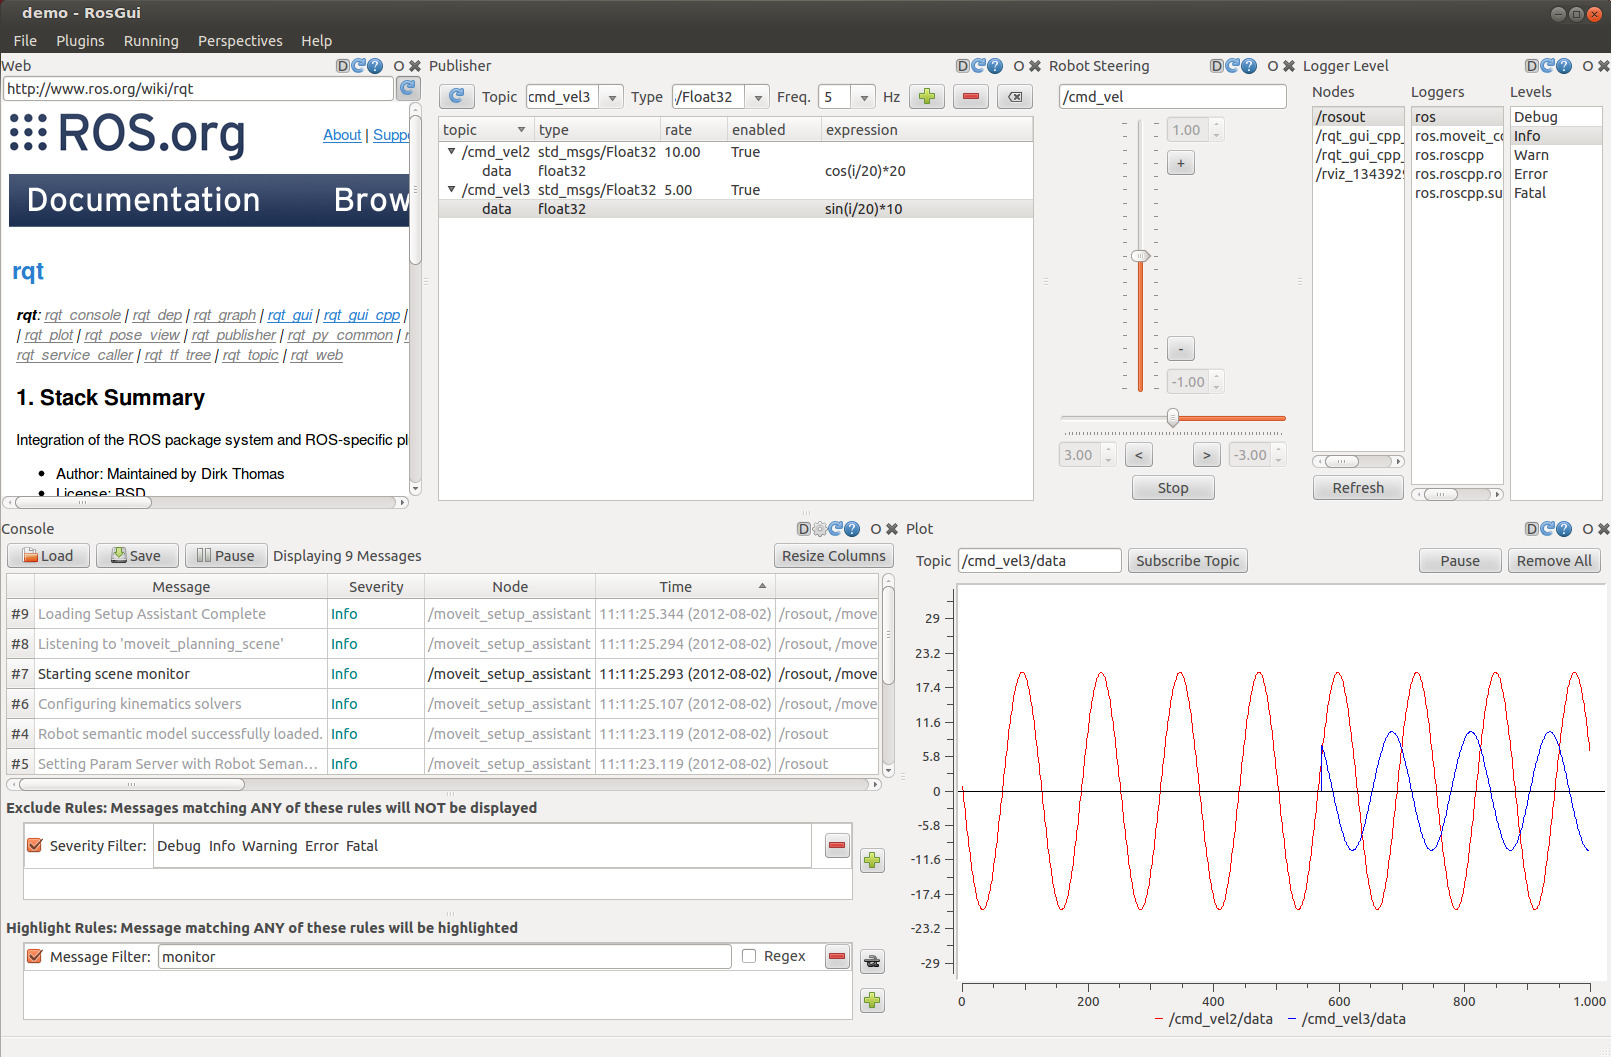
\includegraphics[width=0.8\textwidth]{chapter2/images/ros_gui_example.png}
	\caption{ตัวอย่างการแสดงผลใน rqt }
    \label{fig:ros_gui_example}
\end{figure}


\paragraph*{RViz}
RViz เป็น 3D visualization ของสถานะต่างๆของหุ่นยนต์และสภาพแวดล้อม โดยใช้ไฟล์ URDF เป็นมาตรฐานการแสดงถึงหุ่นยนต์
ซึ่งสามารถที่จะแสดงตำแหน่งปัจจุบันของข้อต่อต่างๆในหุ่นยนต์ได้ สามารถที่จะแสดงค่าเซนเซอร์เป็น marker ได้
การใช้งานจะเป็นเหมือนการบอกพิกัดเฟรม ลักษณะการแสดงผลใน RViz มีหลากหลายรูปแบบไม่ว่าจะเป็น
camera images, depth clouds, laser scans หรือ point clouds อย่างไรก็ตามการแสดงผลใน Rviz
นั้นจะไม่ได้คำนึงถึงแรงที่เข้ามากระทำกับตัวของหุ่นยนต์ แต่ถ้าเป็นการเคลื่อนที่ ที่มีพิกัดเฟรมแล้วสามารถเอามาแสดงได้
ดังรูปที่ \ref{fig:example_visualization_rviz} เป็นเคสของหุ่นยนต์เคลื่อนที่ด้วยล้อ และทำแผนที่ด้วยข้อมูลความลึกที่ได้มาจาก Kinect

\begin{figure}[ht]
    \centering
    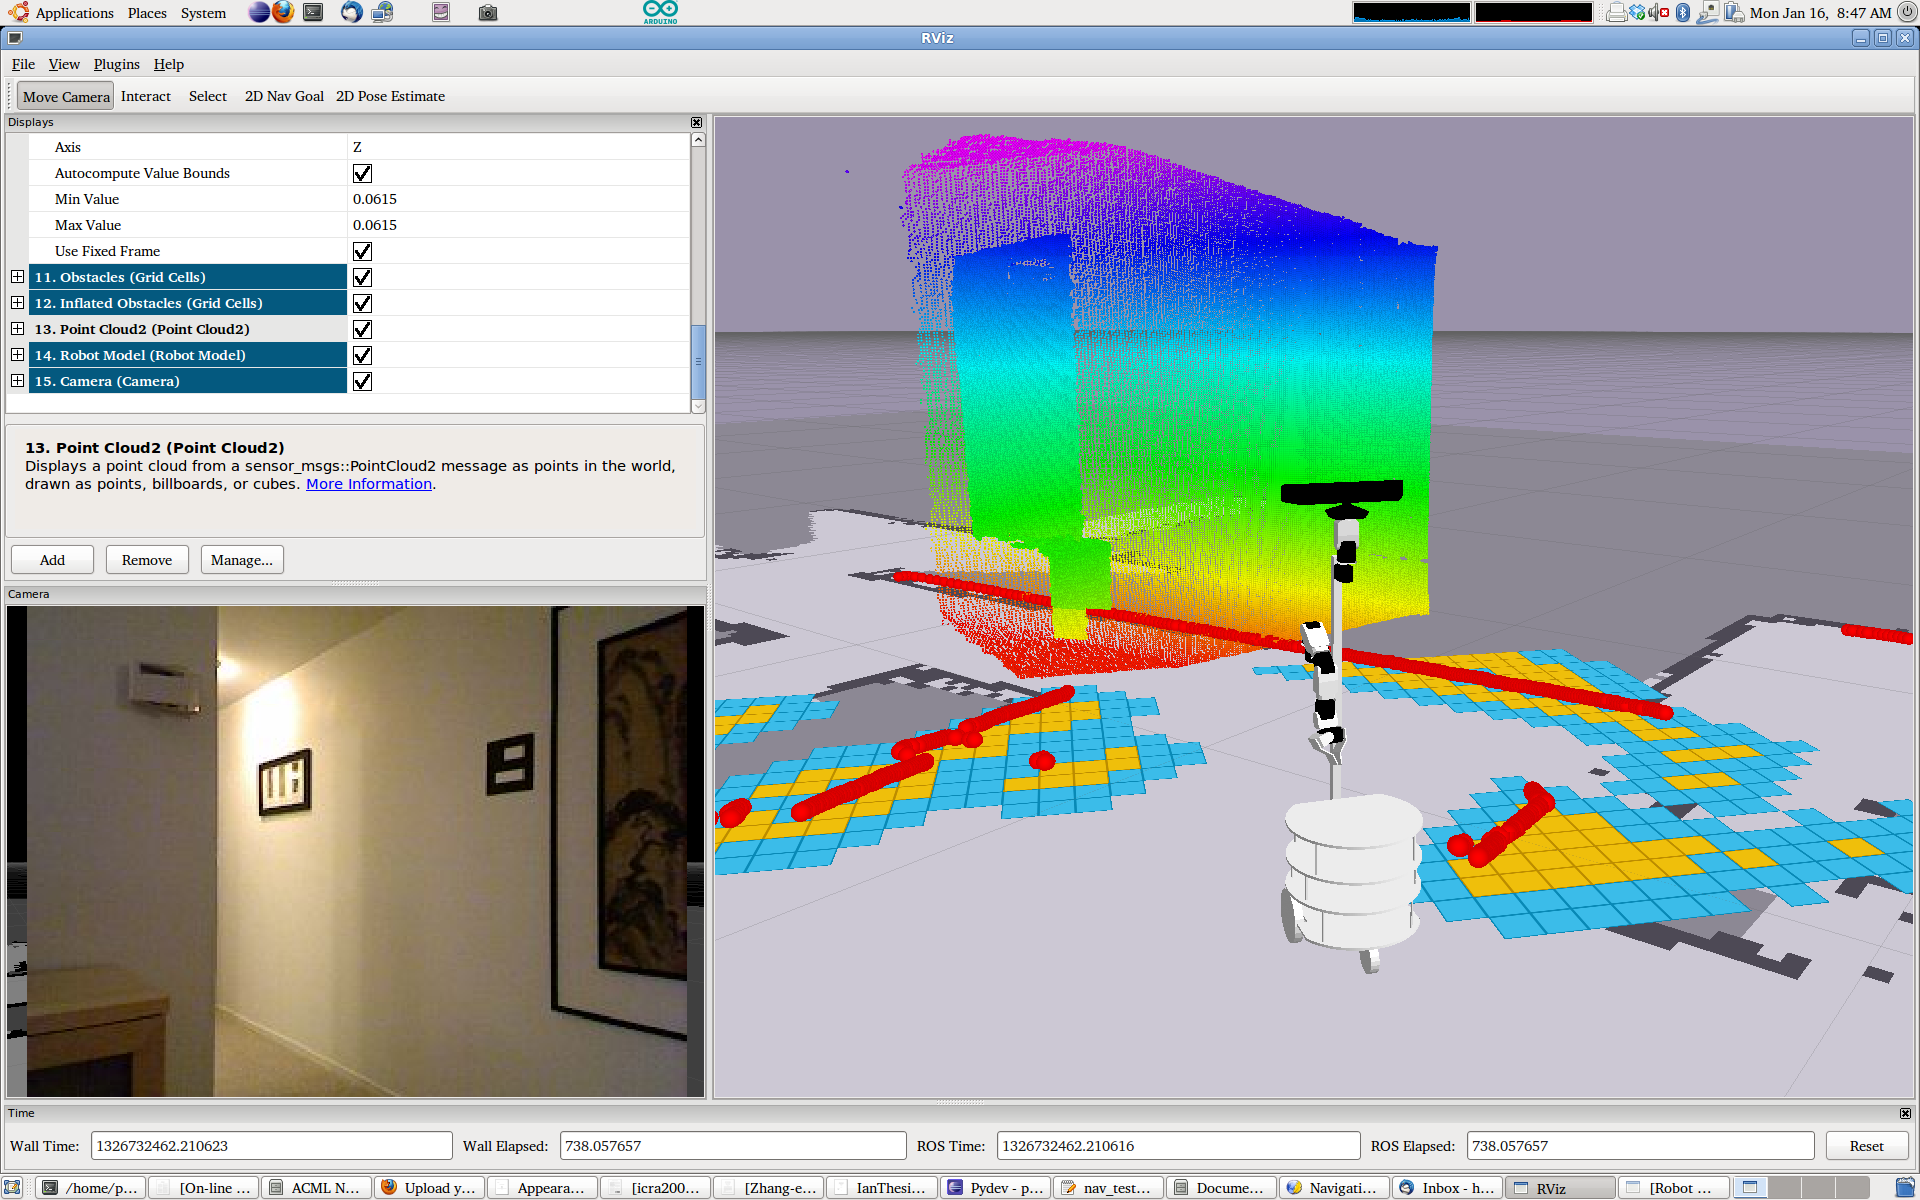
\includegraphics[width=0.8\textwidth]{chapter2/images/nav_test_rviz_2.png}
	\caption{ตัวอย่างการแสดงผลใน RViz}
    \label{fig:example_visualization_rviz}
\end{figure}

% \clearpage
\subsubsection*{Simulation}
Simulation เป็นส่วนที่สำคัญมากสำหรับการพัฒนาโปรแกรมของหุ่นยนต์ เพราะว่าเราสามารถที่จะสร้างโปรแกรมและ
ทดสอบได้โดยไม่จำเป็นต้องมี hardware ซึ่งในส่วนนี้จะช่วยลดความเสียหายจากบักหรือโปรแกรมผิดพลาด ที่อาจจะเกิดขึ้นกับหุ่นยนต์ของเรา 
การจำลองจะช่วยลดเวลาในการพัฒนาลงได้ ระบบจำลองปัจจุบันมีมากมายหลายตัวแต่ ตัวที่ได้รับคำแนะนำมากที่สุดคือ Gazebo
เพราะว่า gazebo สามารถที่จะเชื่อมต่อกับ ROS ได้โดยตรง และนักพัฒนาส่วนใหญ่ใช้ gazebo

การจะใช้ gazebo ได้นั้นเราจะต้องใช้ไฟล์ URDF ซึ่งเป็นไฟล์ที่เอาไว้แสดงหุ่นยนต์ในระบบจำลอง และสามารถที่จะคำนวณหา collision
ให้เราได้อีกด้วย

\begin{figure}[ht]
    \centering
    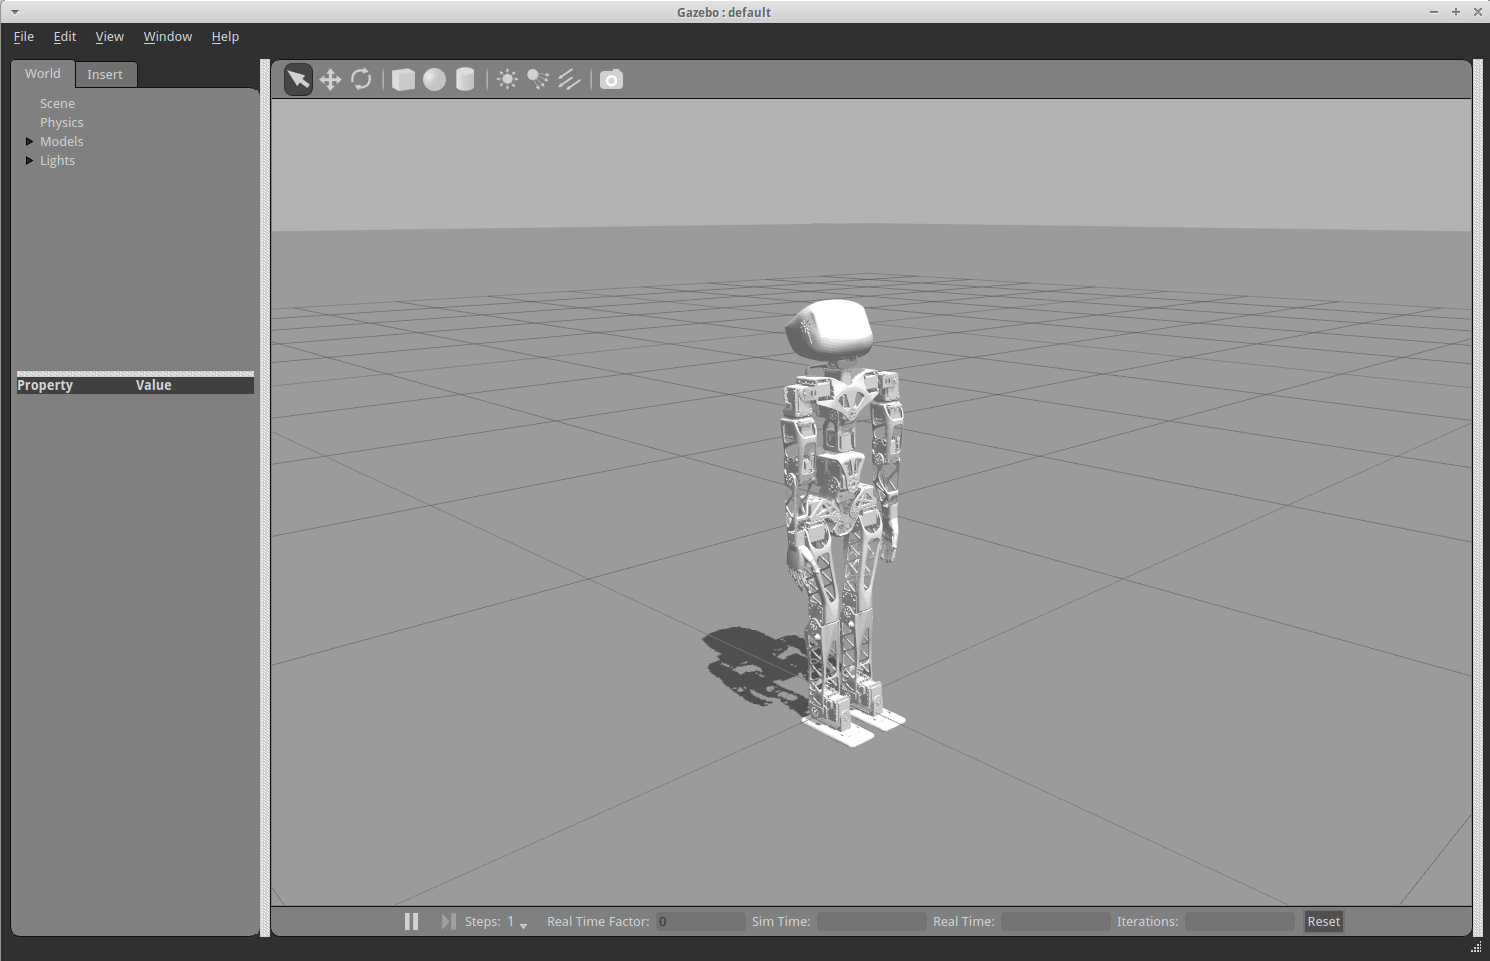
\includegraphics[width=0.8\textwidth]{chapter2/images/gazebo_poppy.png}
	\caption{ตัวอย่างหุ่นยนต์ฮิวมานอยด์ Poppy}
    \label{fig:gazebo_poppy}
\end{figure}



\clearpage
\section{การออกแบบระบบพื้นฐาน}
\subsection{ความแตกต่างของ Operating Systems}

เป็นที่รู้กันโดยทั่วไปว่าฮาร์ทแวร์และซอฟแวร์ของคอมพิวเตอร์นั้นถูกจัดการโดยโปรแกรมในคอมพิวเตอร์ชื่อว่า
operating system (OS) งานพื้นฐานที่ OS ทำก็เช่น การควบคุมและจองหน่วยความจำ
การจัดลำดับความสำคัญของระบบ คอยดูแลควบคุมอุปกรณ์ต่างๆที่เชื่อมต่อเข้ากับคอมพิวเตอร์
การเชื่อมต่อระบบเน็ตเวิร์ค การจัดการไฟล์ข้อมูล อีกทั้งยังรวมไปถึงการให้บริการต่างๆเช่น
การจัดการกระบวนการประมวลผล จัดการไฟล์ของระบบต่างๆ ระบบป้องกัน อื่นๆ

ปัจจุบันมี OS อยู่หลายตัวเช่น Windows, Mac OS X, UNIX, Solaris BS3000, MS-Dos และอื่นๆ
ซึ่งทั้งหมดนี้เป็นส่วนหนึ่งของระบบคอมพิวเตอร์ที่จะคอยช่วยจัดการและควบคุมดูแลการทำงานต่างๆของคอมพิวเตอร์
ระบบคอมพิวเตอร์นั้นอาจจะอยู่ในรูปแบบอื่นๆเช่น เครื่องที่ใช้ทำงาน, เครื่องเซิฟเวอร์, เครื่องคอมพิวเตอร์ส่วนบุคคล, โทรศัพท์เคลื่อนที่,
อุปกรณ์นำทาง หรือแม้กระทั้งระบบที่มีความฉลาดในตัวมันเองเช่น หุ่นยนต์ และ OS
นั้นจะสามารถทำงานบนฮาร์ทแวร์อุปกรณ์ใดๆก็ได้

\subsection{ข้อแตกต่างระหว่าง Open platform กับ Non-open platform}
หุ่นยนต์ Open platform คือ การออกแบบระบบพื้นฐานของหุ่นยนต์ที่เปิดให้ผู้ที่ต้องการศึกษาหรือผู้ใช้ทั่วไปสามารถเข้าถึงข้อมูลต่างๆที่เกี่ยวข้องกับหุ่นยนต์นั้นๆได้
ผู้ใช้สามารถที่จะนำข้อมูลเหล่านั้นมาแก้ไข ปรับปรุง แต่งเติม หรือเรียนรู้และพัฒนาตามได้ด้วยตนเอง 
ซึ่งข้อมูลที่กล่าวมานั้นสามารถหาได้จากเว็บไซต์ของผู้พัฒนาหุ่นยนต์ ปัจจุบันมีหุ่นยนต์ฮิวมานอยด์ที่เป็นเปิดให้เข้าถึงหลายรูปแบบแตกต่างกันไป

ส่วนหุ่นยนต์ Non-open source platform คือหุ่นยนต์ที่สร้างมาเฉพาะเจาะจงสำหรับการวิจัย การสำรวจ หรือการแข่งขันโดยเฉพาะ
ไม่เปิดให้บุคคลภายนอกเข้าศึกษาหรือแก้ไขปรับปรุง ซึ่งทำให้หุ่นยนต์ประเภทนี้ไม่เหมาะสำหรับผู้วิจัยที่จะเรียนรู้และศึกษาด้วยตนเอง เพราะมีขนาดใหญ่
ใช้ทรัพยากรมาก และการออกแบบมีความซับซ้อน เรียนรู้ยากกว่าหุ่นยนต์แบบ Open platform

\subsection{มาตรฐานหน่วยวัดและการบอกพิกัด}
การใช้หน่วยวัดที่ไม่ตรงกันอาจจะทำให้เกิดปัญหาขึ้นได้ เนื่องจากเป็นแพลตฟอร์มนั้นจะมีบุคคลอื่นช่วยกันพัฒนาหลายคน
จึงควรที่จะมีมาตรฐานในการวัดและการกำหนดพิกัดต่างๆที่ตรงกันเพื่อให้เกิดความชัดเจนในการทำความเข้าใจ

\paragraph*{หน่วยวัด}
การวัดนั้นใช้มาตรฐานการวัดเป็น SI Units ซึ่งมาตรฐานนี้ใช้กันอย่างแพร่หลายและเป็นสากล โดยหน่วยการวัดนี้ได้รับการยืนยันจาก
Bureau International des Poids et Mesures ตามตารางที่ \ref{tab:standart_unit}

\begin{table}[!ht]
	\centering
	\begin{tabular}{| l | l | l |}
		\hline
		ปริมาณ (Quantity)                     & หน่วยวัด (Unit)                      & สัญลักษณ์ (Symbol) \\
		\hline
		ความยาว (Length)                    & เมตร (metre)                                 & $m$                                 \\
		มวล (Mass)                                  & กิโลกรัม (kilogram)                  & $kg$                                \\
		เวลา (Time)                               & วินาที (second)                          & $s$                                 \\
		กระแสไฟฟ้า (Electric Current) & แอมแปร์ (ampere)                       & $A$                                 \\
		มุม (Angle)                                 & เรเดียน (radian), องศา (degree) & $rad, deg$                          \\
		ความถี่ (Frequency)                 & เฮิร์ท (Hertz)                           & $Hz$                                \\
		แรง (Force)                                 & นิวตัน (Newton)                          & $N$                                 \\
		กำลัง (Power)                           & วัตต์ (Watt)                               & $W$                                 \\
		แรงดันไฟฟ้า (Voltage)       & โวลต์ (Volt)                               & $V$                                 \\
		อุณหภูมิ (Temperature)            & เซลเซียส (Celsius)                   & ${}^\circ C$                                 \\
		\hline
	\end{tabular}
	\caption{ตารางแสดงหน่วยวัดมาตฐาน}
	\label{tab:standart_unit}
\end{table}

\paragraph*{พิกัดเฟรม}
การบอกทิศทางการหมุนนั้นใช้หลักตามกฏมือขวา โดยการตั้งแกนนั้นหากเทียบกับมือแล้ว X ไปข้างหน้า Y ไปทางซ้าย Z พุ่งขึ้น ดังรูปที่ \ref{fig:right_hand_rule}
\begin{figure}[!ht]
	\centering
	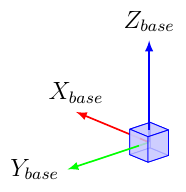
\includegraphics[width=0.15\textwidth]{chapter2/images/right_hand_rule.png}
	\caption{การตั้งแกนตามกฏมือขวา}
	\label{fig:right_hand_rule}
\end{figure}

\subsection{Robot Operating System}
ROS เป็นกรอบการทำงานที่ได้รับความนิยมและมีประสิทธิภาพในการทำงานมากที่สุดในปัจจุบัน เนื่องจาก ROS
ได้รวบรวมซอฟต์แวร์เครื่องมือที่หลากหลายเอาไว้เป็นหมวดหมู่ เช่น การเชื่อมต่อกับฮาร์ดแวร์
การสร้างระบบควบคุมให้กับอุปกรณ์ต่างๆ อีกทั้งสามารถที่จะเขียนโปรแกรมแล้วนำกลับมาใช้ใหม่ได้
ภายในระบบมีกระบวนการรับส่งข้อมูลต่างๆเป็นของตัวเอง ทำให้ช่วยลดความซับซ้อนและเพิ่มประสิทธิภาพในการทำงานกับแพลตฟอร์มของหุ่นยนต์
กระบวนการเขียนโปรแกรมของ ROS นั้นจะใช้รูปแบบ Graph architecture ซึ่งจะทำให้สามารถแบ่งโปรแกรมต่างๆออกเป็นส่วนๆ เช่น
เซนเซอร์หลายๆตัว ระบบควบคุม ระบบวางแผน ระบบขับเคลื่อน ระบบสื่อสารภายนอก ด้วยตัวระบบของ ROS นั้น ไม่ใช้ Real Time OS
แต่อย่างไรก็ตามเราสามารถใช้งานผสมกับ Real Time ได้

ROS ประกอบไปด้วยแพ็กเกจต่างๆ มาประกอบกันเป็น Node โดยมีตัวกลางทำหน้าที่ในการติดต่อสื่อสารระหว่างอุปกรณ์ที่เป็น Node ต่างๆ
ให้สามารถส่งข้อมูลหากันได้ รูปแบบการสื่อสารใน ROS จะใช้หลักการแบบ Publish/Subscribe ทำให้ไม่จำเป็นที่จะต้องระบุโปรแกรมที่จะรับ
ภาษาในการพัฒนามีให้เลือกที่หลากหลาย เช่น C++, Python, Lisp, MATLAB หรือ JavaScript 

\subsubsection*{ประโยชน์จากการใช้ ROS}
ROS เป็นกรอบการทำงาน ที่อยู่ระหว่าง OS และ Robot ทำให้เราไม่ต้องกังวลเรื่องการจัดการระบบภายในเพราะ
ROS จะช่วยจัดการให้เราทั้งหมด ก่อนจะมี ROS นั้น นักวิจัยจะต้องใช้เวลาไปกับพัฒนาพื้นฐานให้หุ่นยนต์
ซึ่งจะต้องมีทักษะทางด้านเครื่องกล ไฟฟ้า และโปรแกรม ซึ่งบ่อยครั้งที่นักวิจัยหรือนักพัฒนานั้นไม่มีความรู้
หรือประสบการณ์ในการสร้างหุ่นยนต์ ทำให้การทำงานเป็นไปด้วยความลำบาก

% ************************** Thesis Chapter3 **********************************
\chapter{การดำเนินงานวิจัย}
วิทยานิพนธ์เรื่องการออกแบบโครงสร้างและพัฒนาระบบพื้นฐานของหุ่นยนต์ฮิวมานอยด์นั้น ผู้วิจัยได้มีการตั้งชื่อให้หุ่นยนต์
โดยใช้ชื่อว่า อุทัย (UTHAI) มาจากภาษาอังกฤษคำว่า Universal Template for Humanoid Algorithm Interface
เพื่อให้สมกับเป็นหุ่นยนต์ฮิวมานอยด์ที่ใช้สำหรับงานวิจัยและพัฒนาต่อยอด

\section{แผนการดำเนินงาน}
โดยจากที่กล่าวไปตอนต้นในบทนำ
การดำเนินงานและการออกแบบการสร้างหุ่นยนต์ฮิวมานอยด์อุทัย มีแผนการทำงานซึ่งแบ่งออกเป็นสามส่วนดังนี้
ส่วนแรกคือ ส่วนของฮาร์ดแวร์ที่เกี่ยวกับโครงสร้างทางกลของหุ่นยนต์ฮิวมานอยด์ เช่น ข้อต่อ ก้านต่อ ฝ่าเท้า
รวมไปถึงระบบอิเล็กทรอนิกส์ ตัวประมวลผลการควบคุม เซนเซอร์ ตัวขับเคลื่อนต่าง ๆ และส่วนที่สองคือ
ส่วนของซอฟท์แวร์ที่เกี่ยวข้องกับการติดต่อสื่อสารกันเบื้องต้น การควบคุมตัวขับเคลื่อนที่ข้อต่อ การอ่านค่าเซนเซอร์
และส่วนที่สาม คือระบบพื้นฐานสำหรับการนำไปศึกษาและพัฒนา โดยจะครอบคลุมไปถึงเอกสารวิธีการใช้งานทั้งในรูปแบบออฟไลน์และออนไลน์

ในการเริ่มต้นทำงานวิจัยเกี่ยวกับฮิวมานอยด์นั้นสิ่งจำเป็นที่ต้องทำในอันดับแรกคือการศึกษาสิ่งที่เคยมีอยู่ หรืองานวิจัยได้ทำเอาไว้แล้ว
ศึกษาทำความเข้าใจใน ข้อดี-ข้อเสีย ของวิธีหรือกระบวนการต่างๆ เพื่อนำมาประยุกต์ใช้กับหุ่นยนต์ฮิวมานอยด์ของเรา
โดยการศึกษานั้นจะเริ่มต้นจากการศึกษาโครงสร้างทางกลของหุ่นยนต์ฮิวมานอยด์ที่มีอยู่แล้วและมีสิ่งที่ต้องดูเป็นพิเศษคือ
วิธีการเชื่อมต่อกันระหว่างก้านต่อและข้อต่อ, จุดที่ใช้ติดตั้งเซนเซอร์ต่างๆ และการเลือกใช้วัสดุให้เหมาะสม
รวมถึงการทำงานของเซ็นเซอร์และตัวขับเคลื่อนที่จำเป็นต้องใช้ในการควบคุมการทำงานของหุ่นยนต์
ในบทนี้ก็จะกล่าวถึงกระบวนการออกแบบและการดำเนินการตามแผนที่วางเอาไว้


%\begin{enumerate}
 %   \item ออกแบบระบบโครงสร้างทางกลของหุ่นยนต์ฮิวมานอยด์ (Solidworks)
 %   \item นำแบบจำลองของหุ่นยนต์เข้าทดสอบการเคลื่อนไหวด้วยโปรแกรมจำลองระบบ (Gazebo)
 %   \item ทดสอบเซนเซอร์ต่าง ๆ เพื่ออ่านค่าออกมาใช้งาน
 %   \item จัดทำชิ้นส่วนโครงสร้างทางกล และประกอบหุ่นยนต์ขึ้นจริง
 %   \item วางแผนระบบการเชื่อมต่อสื่อสาร และการส่งข้อมูลของอุปกรณ์ต่าง ๆ
 %   \item ติดตั้งอุปกรณ์บอร์ดควบคุมการทำงาน และเซนเซอร์เข้ากับตัวหุ่นยนต์
 %   \item จัดทำคู่มือและเอกสารการใช้งานส่วนต่าง ๆ ของหุ่นยนต์ 
%\end{enumerate}


%\clearpage
\section{การออกแบบโครงสร้างของหุ่นยนต์}
การออกแบบทางโครงสร้างทางกลของหุ่นยนต์ฮิวมานอยด์ UTHAIนั้น ผู้วิจัยได้เลือกใช้โปรแกรมออกแบบโครงสร้างเป็นโปรแกรม Solidworks
ที่ช่วยในการพัฒนาแบบจำลองของหุ่นยนต์ฮิวมานอยด์ UTHAI
เนื่องจากโปรแกรม Solidworks เป็นโปรแกรมที่ใช้ในการออกแบบ วาดแบบทางวิศวกรรม
สามารถวิเคราะห์โครงสร้างการรับแรงของแบบจำลองได้ อีกทั้งยังเป็นเครื่องมือที่มีการใช้งานอย่างแพร่หลาย
ทำให้สามารถดาวน์โหลดแบบจำลองต่างๆที่มีคนพัฒนาเข้าเข้ามาใช้ร่วมกับการออกแบบได้ 
และด้วยทางผู้วิจัยมีความคำนึงถึงการพัฒนาต่อยอดเป็นหลัก ดังนั้นการออกโครงสร้างทางกลของหุ่นยนต์ฮิวมานอยด์ UTHAI
จึงถูกออกแบบมาเพื่อให้สามารถรองรับการปรับเปลี่ยน เปลี่ยนแปลง แก้ไขชิ้นส่วนต่างๆของตัวหุ่นยนต์ฮิวมานอยด์ UTHAIได้

\subsection{โครงสร้างหุ่นยนต์}
หุ่นยนต์ที่สร้างขึ้นประกอบด้วยส่วนของลำตัวและส่วนขา ในขาแต่ละข้างออกแบบให้เป็นลักษณะของข้อต่อหมุน (Revolute joint)
เลียนแบบโครงสร้างของมนุษย์ซึ่งประกอบด้วย ส่วนของสะโพกที่มีองศาอิสระจำนวน 3 องศาอิสระ ส่วนของหัวเข่า 1
องศาอิสระและส่วนของข้อเท้า 2 องศาอิสระ รวมขาข้างละ 6 องศาอิสระ ระบบต้นกำลังที่ใช้เป็น Dynamixel servo การออกแบบหุ่นยนต์นั้น
สิ่งแรกที่ต้องทำ คือ การกำหนดโครงสร้างของข้อต่อและก้านต่อขึ้นมาก่อน โดยวาดขึ้นมาเป็นเหมือนโครงกระดูก
ซึ่งโครงสร้างนั้นทางผู้วิจัยได้อ้างอิงมาจากสัดส่วนของมนุษย์จริง ที่ประกอบด้วยส่วนของขาข้างละ 6 องศาอิสระ และมีจุดศูนย์กลาง
อยู่บริเวณกระดูกเชิงกรานของตัวหุ่นยนต์เอง
\begin{figure}[!ht]
    \centering
    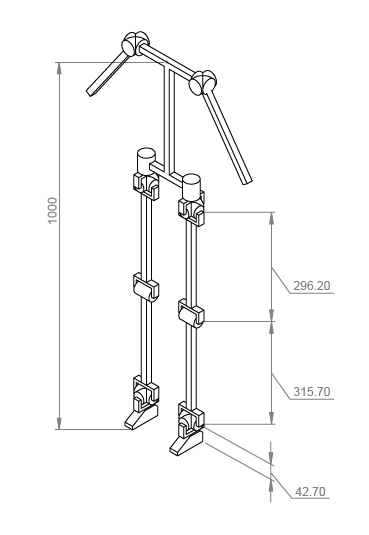
\includegraphics[width=0.35\textwidth]{chapter3/images/uthai_structure1.png}
    \caption{ภาพแสดงแสดงโครงสร้างของหุ่นยนต์ UTHAI}
    \label{fig:uthai_structure1}
\end{figure}

เมื่อเราได้แบบจำลองของหุ่นยนต์ฮิวมานอยด์ออกมาแล้ว ลำดับต่อไปคือการกำหนดตำแหน่งการติดตั้งเซนเซอร์และตัวขับเคลื่อนต่างๆเข้าไป
โดยมี Ground contact sensor ติดตั้งที่ใต้ฝ่าเท้าของหุ่นยนต์, IMU sensor ติดตั้งไว้ให้ใกล้กับจุด COM ของหุ่นยนต์ และ Dynamixel servo
ติดตั้งไว้ที่ข้อต่อในแต่ละข้อต่อ

\begin{figure}[!ht]
    \centering
    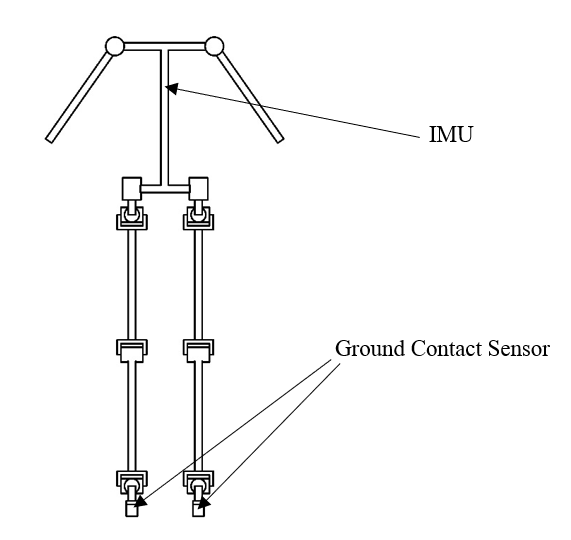
\includegraphics[width=0.5\textwidth]{chapter3/images/uthai_sensor.PNG}
    \caption{ภาพแสดงการติดตั้งเซนเซอร์ในจุดต่างๆ}
    \label{fig:uthai_structure2}
\end{figure}

ส่วนโครงสร้างหุ่นยนต์ฮิวมานอยด์ UTHAI ทางผู้วิจัยเลือกใช้วัสดุหลักเป็น PLA ที่ขึ้นรูปด้วยวิธีการขึ้นรูปสามมิติ
และมีวัสดุเสริมบางชิ้นส่วนจากอลูมิเนียม เนื่องจากจะทำให้โครงสร้างมีน้ำหนักเบา สามารถปรับปรุงแก้ไขง่าย และมีราคาที่สมเหตุสมผล
\begin{table}[ht]
	\centering
	\begin{tabular}{| l | l | l |}
		\hline
		Material & Longitudinal Tensile Strength ($ksi$) & Density ($g/cm^3$) \\
        \hline
        Carbon Fiber & 300 & 1.55 \\
        Steel & 100	& 7.7 \\
        Titanium & 120 & 4.34 \\
        Aluminum & 35 & 2.7 \\
        PLA 3D printing (50 \% infill) & 3.5 & 1.26 \\
        PLA 3D printing (100 \% infill) & 5.5 & 1.26 \\
	    \hline
	\end{tabular}
	\caption{ตารางแสดงสมบัติทางกลของวัสดุต่าง ๆ}
	\label{tab:material_properties}
\end{table}

\clearpage
\subsection{จัดทำชิ้นส่วนโครงสร้างและประกอบ}
ในกาารจัดทำชิ้นส่วนโครงสร้างนั้นทางผู้จัดทำได้คำนึงถึงความแข็งแรงเป็นหลักซึ่งมีความสำคัญมาก
ในการเคลื่อนที่ของหุ่นยนต์ และยังคงต้องมีน้ำหนักที่เบาอีกด้วย\footnote{ Printing Guide [https://filaments.ca/pages/temperature-guide]}
ดังนั้นจึงได้ใช้การขึ้นรูปชิ้นงานด้วยเทคนิค
การพิมพ์ 3 มิติ โดยจะใช้วัสดุหลักเป็นพลาสติก PLA ซึ่งมีความแข็งมากกว่าและขึ้นรูปง่ายกว่าพลาสติกชนิด ABS
เพื่อให้ตอบโจทย์กับหุ่นยนต์แพลตฟอร์มเพื่อพัฒนาต่อยอดในอนาคต ซึ่งผู้ใช้ทุกคนสามารถพิมพ์ขึ้นมาได้ด้วยตนเอง\footnote{ PLA vs ABS [https://www.3dhubs.com/knowledge-base/pla-vs-abs-whats-difference]}

\begin{table}[ht]
	\centering
	\begin{tabular}{| l | l | l |}
		\hline
		Properties & ABS & PLA \\
        \hline
        Tensile Strength & 27 $MPa$ & 37 $MPa$ \\
        Elongation & 3.5 \- 50\% & 6\% \\
        Flexural Modulus & 2.1 \- 7.6 $GPa$ & 4 $GPa$ \\
        Density & 1.0 - 1.4 $g/cm^3$ & 1.3 $g/cm^3$ \\
        Melting Point & 230$°C$ - 240$°C$ & 215$°C$ - 235$°C$ \\ 
        การย่อยสลายทางธรรมชาติ & ไม่ได้ & ได้ (ภายใต้เงื่อนไขที่ถูกต้อง) \\
	    \hline
	\end{tabular}
	\caption{ตารางแสดงสมบัติทางกลของวัสดุพลาสติก}
	\label{tab:plastic_material_properties}
\end{table}
แต่เนื่องจากว่าในปัจจุบันนี้เครื่องพิมพ์ส่วนมากจะไม่รองรับการพิมพ์ชิ้นงานที่มีขนาดใหญ่ ซึ่งมีขนากมากกว่า
30x30x30 ซม. (กว้างxยาวxสูง) ดังนั้นชิ้นงานที่ขึ้นรูปที่มีขนาดใหญ่เกินกว่านี้อาจจะต้องทำการตัดชิ้นงานออกก่อน
แล้วจึงค่อยนำมาประกอบรวมกันทีหลังอีกครั้งหนึ่ง โดยพื้นที่ทำการพิมพ์ของเครื่องพิมพ์ 3 มิติที่มีวางจำหน่าย
และใช้งานแพร่หลายในท้องตลาดแสดงดังตาราง\ref{tab:3dprint_space} \footnote{The truth about 3D printer maximum print areas [https://www.zdnet.com/article/what-manufacturers-dont-want-you-to-know-the-truth-about-3d-printer-maximum-print-areas/]}

\begin{table}[ht]
	\centering
	\begin{tabular}{| l | l | l | l |}
		\hline
		Printer & Actual Width & Actual Depth & Actual Height \\
        \hline
        MakerBot Replicator+ & 292 & 192 & 165 \\
        Ultimaker 3 & 188 & 185 & 200 \\
        LulzBot Mini & 152 & 152 & 158 \\
        Dreammaker Overlord Pro Plus & 79 & 79 & 255 \\
        New Matter MOD-t & 145 & 95 & 125 \\
	    \hline
	\end{tabular}
	\caption{ตารางแสดงขนาดของชิ้นงานที่สามารถพิมพ์ได้ในเครื่องพิมพ์ชนิดต่างๆ}
	\label{tab:3dprint_space}
\end{table}





%%%%%%%%%%%%%%%%%%%%%%%%%%%%%%%%%%%%%%%%%%%%%%%%%%%%%%%%%%%%%%%%%%%%%%%%%%%%%%%
%%%%%%%%%%%%%%%%%%%%%%%%%%%%%%%%%%%%%%%%%%%%%%%%%%%%%%%%%%%%%%%%%%%%%%%%%%%%%%%
%%%%%%%%%%%%%%%%%%%%%%%%%%%%%%%%%%%%%%%%%%%%%%%%%%%%%%%%%%%%%%%%%%%%%%%%%%%%%%%
\clearpage
\subsection{อุปกรณ์ที่ใช้ในหุ่นยนต์ฮิวมานอยด์ UTHAI}

\subsubsection*{Dynamixel servo EX-106+}
Dynamixel EX-106+ เป็นตัวขับเคลื่อนที่นิยมใช้ในปัจจุบัน ซึ่งเป็นเซอร์โวมอเตอร์ที่เหมาะสำหรับทำหุ่นยนต์โดยเฉพาะ
ภายในประกอบไปด้วย มอเตอร์กระแสตรง ชุดเฟืองมอเตอร์ ไดรเวอร์คอนโทรเลอร์ สามารถเชื่อมต่อกันผ่าน BUS RS-485
\footnote{ Robot Actuator [http://support.robotis.com/en/product/actuator/dynamixel/ex\_series/ex-106.htm] }
มีการควบคุมแบบ PID สามารถที่จะอ่านค่าความเร็ว
แรงดันไฟฟ้า กระแสไฟฟ้า อุณหภูมิ ตำแหน่ง และแรงบิดจากมอเตอร์ทุกตัวได้ แต่ละมอเตอร์แต่ละตัวจะมีบอร์ดควบคุมของตัวเอง
เราสามารถที่จะจ่ายไฟให้มอเตอร์และควบคุมผ่าน Serial ได้เลย

การทำงานของตัวขับเคลื่อนนี้สามารถทำได้ 2 รูปแบบคือ\footnote{ EX-106+ Mode [http://www.trossenrobotics.com/dynamixel-ex-106-robot-actuator.aspx] }

\paragraph*{Joint Mode}
สามารถที่จะควบคุม Torque Speed และ position ได้ความละเอียดในการควบคุม 10-bit (0-1023) หมุนได้อยู่ในช่วง 0-250 องศา

\paragraph*{Wheel Mode}
สามารถที่จะควบคุม Torque Speed และ direction ได้ ความละเอียดของความเร็วมอเตอร์เท่ากับ 10bit (0-1023) สามารถหมุนได้ครบ 360 องศาได้

\begin{figure}[!ht]
    \centering
    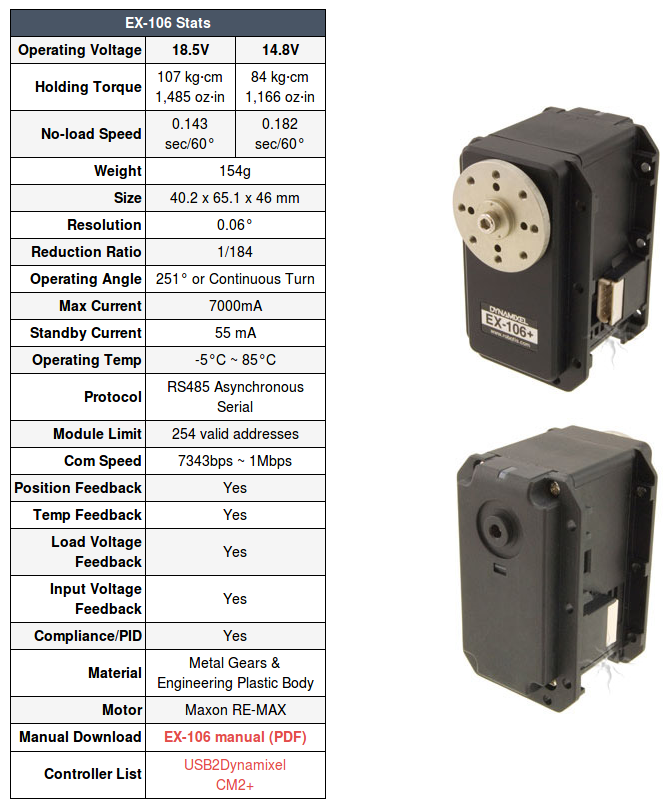
\includegraphics[width=0.75\textwidth]{chapter3/images/dxl_ex106.png}
    \caption{แสดงประสิทธิภาพของมอเตอร์ EX-106+}
    \label{fig:dxl_ex106}
\end{figure}


\clearpage
\subsubsection*{USB2Dynamixel connector}
USB2Dynamixel เป็นอุปกรณ์สำหรับเชื่อมต่อหน่วยประมวลผลระดับสูง (Odroid) กับดิจิตอลเซอร์โวโดยจะเชื่อมต่อ ผ่านพอร์ท USB ของ Odroid ไปยังดิจิตอลเซอร์โว
ผ่านสาย 2 เส้น คือ D+ และ D-
เป็นการเชื่อมต่อแบบ RS-485\footnote{USB2Dynamixel [http://support.robotis.com/en/product/auxdevice/interface/usb2dxl\_manual.html]}
ืทำให้สามารถส่งข้อมูลระยะทางไกลได้ และสามารถที่จะมีหลายอุปกรณ์บนสายเส้นเดียวกันได้

\begin{figure}[!ht]
    \centering
    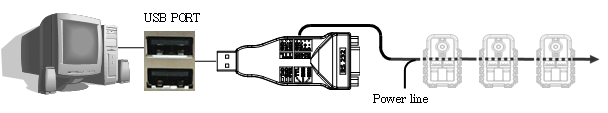
\includegraphics[width=0.75\textwidth]{chapter3/images/dynamixel2pc.png}
    \caption{ภาพแสดงการติดต่อสื่อสารระหว่างคอมพิวเตอร์กับมอเตอร์ Dynamixel}
    \label{fig:dynamixel2pc}
\end{figure}

ในการต่อใช้งานนั้นผู้ใช้งานจำเป็นต้องเลือกการติดต่อสื่อสารระหว่าง คอมพิวเตอร์กับมอเตอร์
ซึ่งการติดต่อสื่อสารนั้นหากใช้ USB2Dynamixel ตัวอุปกรณ์ชิ้นนี้ได้แบ่งการติดต่อสื่อสารออกเป็น 3 รูปแบบคือ
\vspace{-10pt}
\begin{enumerate}[label=\arabic*, leftmargin=1.5cm]
    \setlength\itemsep{-0.25em}
    \item TTL Communication : สำหรับดิจิตอลเซอร์โวที่ใช้พอร์ทชนิด 3-pin เช่นในตระกูล AX Series เช่น AX-S1 AX-12+ ฯลฯ
    \item RS485 Communication : สำหรับดิจิตอลเซอร์โวที่ใช้พอร์ทชนิด 4-pin เช่นในตระกูล DX Series เช่น RX Series, EX Series ฯลฯ
    \item RS232 Communication : ใช้สำหรับติดต่อสื่อสารกับคอนโทรลเลอร์ผ่านสายเคเบิล
\end{enumerate}
\vspace{-15pt}
\begin{figure}[!ht]
    \centering
    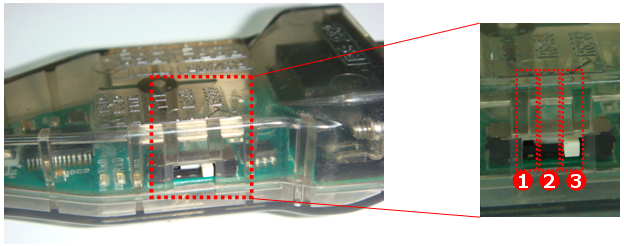
\includegraphics[width=0.5\textwidth]{chapter3/images/useusb2dynamixel.png}
    \caption{ภาพแสดงการเลือกโหมดใช้งานของ USB2Dynamixel}
    \label{fig:useusb2dynamixel}
\end{figure}

แต่จากการทดลองนำมาใช้ผู้วิจัยพบว่า Dynamixels ที่ใช้ในการทำงานวิจัยครั้งนี้เป็นชนิด 4 pin ซึ่งใช้ RS485 ในการติดต่อสื่อสาร
และด้วยขนาดของตัว USB2Dynamixel มีขนาดที่ใหญ่ทำให้การทำงานมีความลำบากในการติดตั้งลงบนตัวของหุ่นยนต์
จึงได้ทำการเปลี่ยนเป็น USB to RS485 แทน
\begin{figure}[!ht]
    \centering
    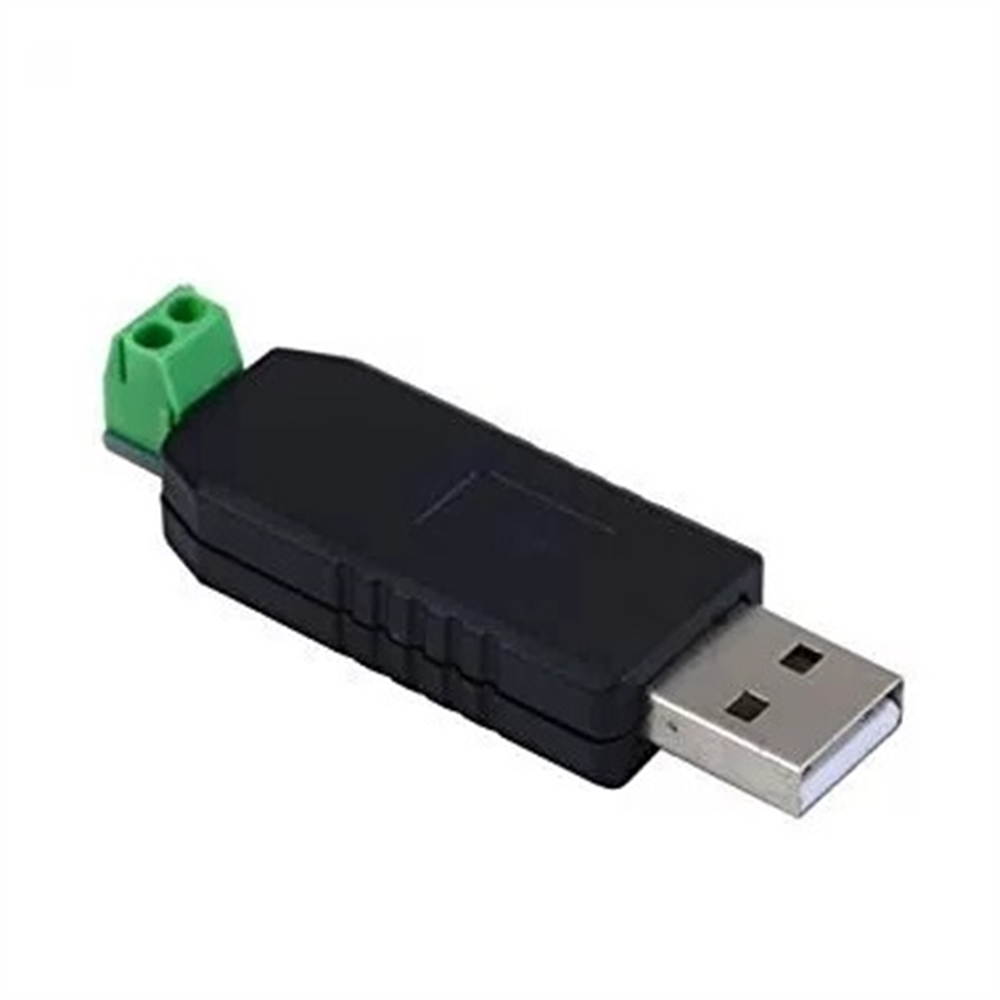
\includegraphics[width=0.3\textwidth]{chapter3/images/usb2rs485.jpg}
    \caption{USB2RS485 Module}
    \label{fig:usb2rs485}
\end{figure}

\clearpage
\subsubsection*{Inertial Measurement Unit (IMU)}
ในการทำวิจัยครั้งนี้ผู้จัดทำได้เลือกนำเซนเซอร์ MPU-9250 มาใช้ในการอ่านค่ามุมเอียงของหุ่นยนต์เพื่อใช้ในการคุมเสถียรภาพของหุ่นยนต์
โดยเซนเซอร์ตัวนี้สามารถวัดค่าได้ 9 แกนคือ วัดค่าความเร็วเชิงมุม (gyroscope) 3 แกน วัดค่าความเร่งเชิงเส้น(accelerometer) 3 แกน
และวัดค่าสนามแม่เหล็กโลก (magnetometer) 3 แกน ซึ่งเซนเซอร์ตัวนี้จะติดตั้งบริเวณส่วนของลำตัวหุ่นยนต์
เนื่องจากว่าจะเป็นจุดที่สามารถบ่งบอกได้ถึงการเคลื่อนที่และมุมเอียงของหุ่นยนต์ในขณะนั้นได้ดีที่สุด\footnote{ MPU-9250 [http://www.arduiner.com/en/gy-series-axis-accellerometers/6924-gy9255-mpu9255-sensor-module-alternative-mpu9150-mpu9250-3809200640200.html] }
\begin{figure}[!ht]
    \centering
    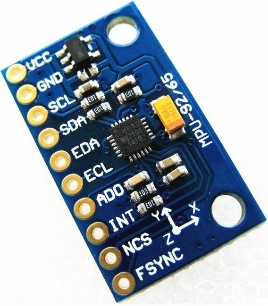
\includegraphics[width=0.2\textwidth]{chapter3/images/mpu9250.jpeg}
    \caption{แสดงเซนเซอร์ IMU MPU9250}
    \label{fig:mpu9250}
\end{figure}

\subsubsection*{Wi-Fi Adapter}
ตัวรับสัญญาณ wifi ชนิดพกพาเพื่อใช้ในการติดต่อสื่อสารระหว่างคอมพิวเตอร์ที่ติดตั้งอยู่บนตัวของหุ่นยนต์
และคอมพิวเตอร์ที่เป็นตัวสั่งการซึ่งอยู่นอกตัวของหุ่นยนต์ ซึ่งในงานวิจัยนี้
จะใช้ส่งข้อมูลที่ได้หลังจากการประมวลผลบนคอมพิวเตอร์ไปยังตัวหุ่นยนต์ เช่น การวางแผนการเดิน การคำนวนพลศาสตร์ของหุ่นยนต์
และอื่นๆ โดยการส่งข้อมูลไปยังคอมพิวเตอร์ที่อยู่บนตัวหุ่นยนต์นั้นจะมีตัวกลางในการรับส่งสัญญาณ
คือ ตัวกระจายสัญญาณ (wifi router)
\begin{figure}[!ht]
    \centering
    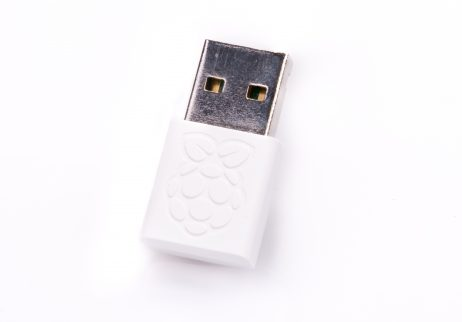
\includegraphics[width=0.3\textwidth]{chapter3/images/rpi_wifi_adaptor.jpg}
    \caption{ตัวรับสัญญาณ wifi ของ RaspberryPi}
    \label{fig:rpi_wifi_adaptor}
\end{figure}
\begin{figure}[!ht]
    \centering
    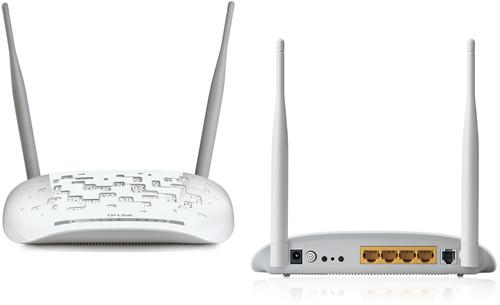
\includegraphics[width=0.3\textwidth]{chapter3/images/wifi_router.jpg}
    \caption{ตัวกระจายและรับส่งสัญญาณ wifi}
    \label{fig:wifi_router}
\end{figure}


\clearpage
\subsubsection*{Ground contact sensor}
เซนเซอร์ตรวจหน้าสัมผัสที่พื้นเป็นเซนเซอร์ที่ถูกติดตั้งบริเวณฝ่าเท้า เพื่อตรวจสอบการเดินของหุ่นยนต์ฮิวมานอยด์ว่าขณะนี้มีการสัมผัสของฝ่าเท้าของหุ่นยนต์กับพื้นหรือไม่ 
ซึ่งในงานวิจัยนี้ได้ใช้หลักการตัวตรวจจับแรงกดแบบค่าความต้านทานหรือ Force Sensing Resistor (FSR) ที่ใช้เทคโนโลยีฟิล์มโพลีเมอร์แบบหนา (Polymer Thick Film) 
โดยแรงดันไฟฟ้าที่ตกคร่อมตัวตรวจจับจะลดลง เมื่อมีแรงกดมากระทำบนแผ่นตรวจจับ มีโครงสร้างของตัวตรวจจับแสดง ดังรูปที่ \ref{fig:FSRarchitec}
\begin{figure}[!ht]
    \centering
    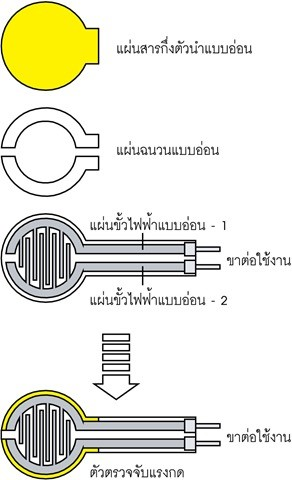
\includegraphics[width=0.35\textwidth]{chapter3/images/FSRarchitec.jpg}
    \caption{ลักษณะโครงสร้างของตัวตรวจจับแรงกด FSR}
    \label{fig:FSRarchitec}
\end{figure}

ประกอบด้วยแผ่นสารกึ่งตัวนำแบบอ่อนที่เป็นตัวกำหนดค่าความต้านทานไฟฟ้าประกบ เข้ากับแผ่นขั้วไฟฟ้าแบบอ่อน โดยมีแผ่นฉนวนแบบอ่อนคั่นกลาง 
ทำให้เกิดค่าความต้านทานไฟฟ้าขึ้นระหว่างขาต่อใช้งาน เมื่อมีการกดลงบนแผ่นขั้วนำไฟฟ้า จะทำให้เกิดการสัมผัสระหว่างสารกึ่งตัวนำกับขั้วไฟฟ้า
ส่งผลให้ค่าความต้านทานไฟฟ้าเกิดการเปลี่ยนแปลง ดังแสดงกระบวนการทำงานในรูปที่ \ref{fig:FSRfunction}
\begin{figure}[!ht]
    \centering
    \includegraphics[width=0.5\textwidth]{chapter3/images/FSRfunction.jpg}
    \caption{การทำงานของตัวตรวจจับแรงกด FSR}
    \label{fig:FSRfunction}
\end{figure}

แนวคิดการออกแบบหลัก คือการออกแบบให้สามารถติดตั้งกับตัวหุ่นยนต์ได้เลย ไม่ต้องเชื่อมต่อสายไฟและสายส่งข้อมูลใหม่ โดยให้ใช้สายไฟไฟเลี้ยง 
และสายสัญญาณชุดเดียวกับตัวขับเคลื่อน Dynamixel Servo Mo-tor ซึ่งมีการติดต่อกันในลักษณะเป็นบัสแบบ RS-485 ดังนั้นแล้วผู้เขียนจึงเลือกที่จะทำโมดูลขึ้นมาใหม่ 1 โมดูล 
เพื่อที่ใช้ในการอ่านค่า Ground Contact Sensor ของหุ่นยนต์โดยเฉพาะ โดยมีการติดต่อรูปแบบบัส RS-485 ใช้ลักษณะการติดต่อสื่อสาร(Protocol) เดียวกับตัวขับเคลื่อน Dynamixel 
และมีการพัฒนาจาก Arduino ซึ่งให้สามารถอ่านค่าได้ทั้ง Analog และ Digital ได้ อีกทั้งรองรับการต่อ Sensor แบบ Force sensitive resistor จำนวน 4 ตัว.
\begin{figure}[!ht]
  \centering
  \includegraphics[width=0.8\textwidth]{chapter3/images/FSR_schematic.png}
  \caption{Schematic ของวงจร Ground Contact Sensor}
  \label{fig:FSR_schematic}
\end{figure}

\begin{figure}[!ht]
  \centering
  \includegraphics[width=0.8\textwidth]{chapter3/images/complete_FSR.png}
  \caption{แผงวงจร Ground Contact Sensor ที่ประกอบเสร็จแล้ว}
  \label{fig:complete_FSR}
\end{figure}

\clearpage
เซนเซอร์ที่เลือกใช้คือ Force Sensitive Resistor (FSR) เป็นเซนเซอร์ที่มีค่าความต้านทานภายในตัวเอง โดยเซนเซอร์นี้มีหลักการทำงานคือ 
ค่าความต้านทานทางไฟฟ้าของตัวเซนเซอร์จะเปลี่ยนแปลงเมื่อมีแรงเข้ามากระทำกับหน้าสัมผัส เมื่อมีแรงเข้ามากระทำมาก จะทำให้ค่าความต้านทานต่ำ 
หากไม่มีแรงเข้ามากระทำจะทำให้มีค่าความต้านทานสูง และเมื่อมีการนำเซนเซอร์นี้มาต่อกับตัวต้านทานที่มีค่าคงที่ ในรูปแบบของ Voltage Divider 
ดังรูปที่ \ref{fig:FSR_schematic} จะทำให้สามารถอ่านค่าแรงดันไฟฟ้าที่เปลี่ยนแปลงตามแรงที่เกิดขึ้นกับหน้าสัมผัสของเซนเซอร์ FSR ได้ 

\begin{figure}[!ht]
  \centering
  \includegraphics[width=0.3\textwidth]{chapter3/images/FSR.jpg}
  \caption{Force Sensitive Resistor (FSR) ขนาด 0.5 นิ้ว}
  \label{fig:FSR}
\end{figure}

ข้อดีของ FSR นั้นคือ เป็นเซนเซอร์ที่ถูกพัฒนาและออกแบบมาเพื่อใช้สำหรับการวัดแรงโดยตรง จึงทำให้ใช้งานได้ง่าย และสะดวก ในราคาที่ถูกกว่า 
เมื่อเทียบกับเซนเซอร์ Load cell ที่มีราคาสูงและการใช้งานจำเป็นที่จะต้องมีวงจรขยายสัญญาณที่ใช้ในการอ่านค่าการบิดของวัสดุจาก 
แต่ FSR นั้นก็มีข้อเสียเช่นกันคือ ความไม่ทนทานต่อการขีดข่วน เนื่องจากตัวเซนเซอร์ถูกทำมาจากฟิล์มพลาสติกบางๆ ซึ่งหากเกิดการขีดข่วนเกิดขึ้นแล้วอาจทำให้ฟิล์มฉีกขาดได้ 
หากฟิล์มขาดจะทำให้ค่าความต้านทานออกมาไม่เหมือนเดิม ดังนั้นทางผู้เขียนจึงเลือกที่จะออกแบบโครงครอบสำหรับเซนเซอร์ FSR เพื่อป้องกันจากการถูกขีดข่วนจากภายนอก







%%%%%%%%%%%%%%%%%%%%%%%%%%%%%%%%%%%%%%%%%%%%%%%%%%%%%%%%%%%%%%%%%%%%%%%%%%%%%%%
\clearpage
\subsection{การเชื่อมต่อตัวขับเคลื่อนและตัวรับรู้}
โครงสร้างของหุ่นยนต์ฮิวมานอยด์ UTHAIจะมีขาสองข้างทำให้เกิดองศาอิสระ 12 องศาอิสระ
จึงใช้ดิจิตอลเซอร์โวทั้งหมด 12 ตัว ดิจิตอลเซอร์โวทุกตัวเชื่อมต่อกันแบบสายโซ่เดซี่ (daisy chain) ดังรูปที่ \ref{fig:dynamixel_connect}
ข้างหนึ่งของมอเตอร์ตัวแรกเชื่อมต่อกับแบตเตอร์รี่ 12V และอีกข้างต่อกับ USB2RS485 เพื่อต่อไปยังตัวประมวลผลระดับสูง (Odroid)
และเซนเซอร์หน่วยวัดความเฉื่อย กับเซนเซอร์ตรวจจับหน้าสัมผัสที่พื้นเชื่อมต่อกับตัวประมวลผลระดับต่ำ (Nucleo F411RE)
ดังรูปที่ \ref{fig:odroid2dynamixel}
\begin{figure}[!ht]
    \centering
    \includegraphics[width=0.7\textwidth]{chapter3/images/dynamixel_connect.png}
    \caption{การเชื่อมต่อกันระหว่างดิจิตอลเซอร์โว}
    \label{fig:dynamixel_connect}
\end{figure}
\begin{figure}[!ht]
    \centering
    \includegraphics[width=0.9\textwidth]{chapter3/images/odroid2dynamixel.JPG}
    \caption{การเชื่อมต่อระหว่างตัวรับรู้ ตัวประมวลผล และตัวขับเคลื่อน}
    \label{fig:odroid2dynamixel}
\end{figure}


%%%%%%%%%%%%%%%%%%%%%%%%%%%%%%%%%%%%%%%%%%%%%%%%%%%%%%%%%%%%%%%%%%%%%%%%%%%%%%%
\clearpage
\subsection{การตั้งค่าดิจิตอลเซอร์โว}

\begin{wrapfigure}{l}{0.2\textwidth}
    \includegraphics[width=0.9\linewidth]{chapter3/images/roboplus/roboplus.jpg} 
    \caption*{Roboplus 1.0}
\end{wrapfigure}

ก่อนที่จะเชื่อมต่อดิจิตอลเซอร์โวเข้ากับระบบประมวลผล จำเป็นที่จะต้องมีการตั้งค่า ID, Baudrate, Joint limited 
ของดิจิตอลเซอร์โว โดยการตั้งค่าพารามิเตอร์ของดิจิตอลเซอร์โวนั้น ผู้วิจัยจะใช้โปรแกรมที่มีชื่อว่า
Roboplus 1.0 ซึ่งเป็นเครื่องมือจากบริษัท Robotis ที่จำหน่ายดิจิตอลเซอร์โวนี้ โดยจะช่วยให้สามารถติดต่อกับดิจิตอลเซอร์โว
ตั้งค่าพารามิเตอร์ได้ แต่โปรแกรม Roboplus 1.0 นี้ใช้ได้เฉพาะใน Windows OS เท่านั้น ซึ่งสามารถดาวน์โหลดโปรแกรมได้จากหน้าเว็บไซต์ Robotis\footnote{http://www.robotis.us/roboplus1/}
เมื่อดาวน์โหลดโปรแกรมและติดตั้งเรียบร้อยแล้ว ให้เชื่อมต่อดิจิตอลเซอร์โวกับคอมพิวเตอร์ด้วย USB2RS485
และตั้งค่าพารามิเตอร์โดยทำตามขั้นตอน ดังรูปต่อไปนี้
\begin{figure}[!ht]
    \centering
    \includegraphics[width=\textwidth]{chapter3/images/roboplus/roboplus0.jpg}
    \caption*{เชื่อมต่อดิจิตอลเซอร์โวเข้ากับคอมพิวเตอร์ด้วย USB2RS485}
\end{figure}
\begin{figure}[!ht]
    \centering
    \includegraphics[width=0.25\textwidth]{chapter3/images/roboplus/roboplus1.PNG}
    \caption*{เปิดโปรแกรม Roboplus 1.0}
\end{figure}
\begin{figure}[!ht]
    \centering
    \includegraphics[width=0.55\textwidth]{chapter3/images/roboplus/roboplus2.PNG}
    \caption*{กดเข้าไปที่ Dynamixel Wizard}
\end{figure}
\begin{figure}[!ht]
    \centering
    \includegraphics[width=0.55\textwidth]{chapter3/images/roboplus/roboplus3.PNG}
    \caption*{เลือก COM Port ให้ตรงกับ USB2RS485 จากนั้นกด Connect}
\end{figure}
\begin{figure}[!ht]
    \centering
    \includegraphics[width=0.55\textwidth]{chapter3/images/roboplus/roboplus4.PNG}
    \caption*{กดเลือกที่ช่อง 1Mbps แล้วกด Start searching}
\end{figure}
\begin{figure}[!ht]
    \centering
    \includegraphics[width=0.55\textwidth]{chapter3/images/roboplus/roboplus5.PNG}
    \caption*{เมื่อเห็นทางด้านซ้ายมือโผล่ ID มอเตอร์ขึ้นมา หากขึ้นแล้วก็สามารถกด Stop Searching ได้}
\end{figure}
\begin{figure}[!ht]
    \centering
    \includegraphics[width=0.55\textwidth]{chapter3/images/roboplus/roboplus6.PNG}
    \caption*{ทดสอบสั่งการมอเตอร์ที่ Addr 30 Goal position ว่าทิศทางถูกต้องหรือไม่}
\end{figure}
\begin{figure}[!ht]
    \centering
    \includegraphics[width=0.55\textwidth]{chapter3/images/roboplus/roboplus7.PNG}
    \caption*{ถ้าทิศทางไม่ถูกต้องสามารถที่จะปรับได้ที่ Addr 10 Drive mode}
\end{figure}

%%%%%%%%%%%%%%%%%%%%%%%%%%%%%%%%%%%%%%%%%%%%%%%%%%%%%%%%%%%%%%%%%%%%%%%%%%%%%%%
\clearpage
\subsection{การเชื่อมต่อบอร์ดประมวลผล}
การเชื่อมต่อระหว่างบอร์ดประมวลผลระดับล่างกับบอร์ดประมวลผลระดับสูง โดยจะเชื่อมต่อกันผ่านสาย USB
และส่งข้อมูลหากันผ่านซีเรียลโดยใช้ rosserial นอกจากจะมีบอร์ดประมวลผลแล้วยังมีบอร์ดที่เอาไว้ใช้สำหรับควบคุม
ดิจิตอลเซอร์โวเพื่อเผื่อเอาไว้สำหรับเปลี่ยนให้ ตัวประมวลผลควบคุมระดับล่างเป็นตัวสั่งการมอเตอร์
ดัวรูปที่ \ref{fig:uthai_controller}

\begin{figure}[!ht]
    \centering
    \includegraphics[width=0.4\textwidth]{chapter3/images/uthai_controller.jpg}
    \caption{การเชื่อมต่อกันระหว่างตัวประมวลผล}
    \label{fig:uthai_controller}
\end{figure}






\clearpage
\section{การออกแบบโปรแกรมด้วย ROS}
\subsection{Modelling}
หลังจากที่เราได้ออกแบบและโมเดลหุ่นยนต์ของเราขึ้นมาที่ใช้ CAD tools ต่างๆ เช่น AutoCAD, SolidWorks, Blender
หรืออื่นๆ ก็เพื่อที่จะนำมาใช้ในการทำ Simulation การที่เราทำ Simulation นั้นก็จะสามารถมองเห็นหุ่นยนต์
และเห็นการทำงานของหุ่นยนต์เราก่อนที่เราจะสร้างมันขึ้นมาจริงๆ หุ่นยนต์จำลองที่เราสร้างขึ้นมานั้นควรที่จะมีลักษณะให้ใกล้เคียงกับของจริงมากที่สุด
ไม่ว่าจะเป็นรูปร่าง รูปทรง น้ำหนักต่างๆ 

\subsubsection{ROS packages for robot modelling}
ROS นั้นได้ให้เครื่องมือที่ช่วยให้เราสามารถสร้าง 3D robot models ได้
ใน ROS มี meta package ที่ชื่อว่า robot\_model ซึ่งข้างในมี package ต่างๆที่ใช้สำหรับสร้าง 3D robot models
        
\paragraph*{urdf}
เป็น 1 ในหลายๆ package ที่อยู่ใน robot\_model, urdf เป็น xml ไฟล์ที่เอาไว้ใช้บอกลักษณะของหุ่นยนต์ ย่อมาจาก Unified Robot Description Format(URDF)
เราสามารถระบุ robot model, sensors และ working environment โดยใช้ URDF การบอกนั้นจะสามารถบอกเป็นเหมือน tree structure ของ link ต่างๆในตัวหุ่นยนต์ สามารถบอก rigid link เชื่อมต่อกันผ่าน joints แต่ถ้าเป็น flexible link จะไม่สามารถบอกได้โดยใช้ urdf

\subparagraph*{joint\_state\_publisher}
เครื่องมือนี้มีประโยชน์มากในการ model robot URDF เพราะมันสามารถหา joints ทุก joint ที่ไม่ใช่ fixed joints มาแสดงเป็น GUI sliders ทำให้เราสามารถเลื่อนๆหมุนๆไปมาได้ อีกทั้งยังสามารถใช้งานร่วมกับ visualize RViz

\subparagraph*{robot\_state\_publisher}
เป็นเครื่องมือที่ใช้ในการ publish 3d pose ของ link ต่างๆใน urdf การ ยublish นั้นจะใช้ ROS tf(transform) ROStf คือการหาความสัมพันธ์ระหว่าง frame ของหุ่นยนต์

\subparagraph*{xacro}
ย่อมาจาก XML Macros หรือเราสามารถเรียกอีกอย่างว่า URDF plus add-ons. ซึ่งการทำงานเหมือนกับ urdf แต่ทำให้ไฟล์ urdf สั้นกว่า อ่านง่ายกว่า และสามารถใช้เพื่อทำให้สร้างหุ่นยนต์ที่มีความซับซ้อนง่ายขึ้น เราสามารถแปลงไฟล์ xacro เป็น urdf ได้

\subsubsection{URDF}
ในส่วนนี้จะเป็นการอธิบายระบบทางกลของหุ่นยนต์ฮิวมานอยด์เป็นไฟล์ที่ใช้ร่วมกับ ROS ได้ เพื่อที่จะสามารถนำไปใช้กับ Simulation ในอนาคตได้
ในการอธิบายระบบทางกลนั้นผู้วิจัยได้ใช้ไฟล์ URDF (Universal Robotics Description Format) ซึ่งใช้ภาษาการเขียนเป็น XML ในการบอกส่วนประกอบแต่ละส่วนของหุ่นยนต์

\subsubsection*{Link}
ในไฟล์ URDF แต่ละชิ้นส่วนของหุ่นยนต์เราจะเรียกว่า link แล้วใน link จะประกอบไปด้วยส่วนย่อยๆ
3 ส่วนคือ <inertia> ที่เอาไว้บอกถึงค่าตัวแปรทางฟิสิกส์, <visual> ที่เอาไว้แสดงผลให้เราเห็น, 
<collision> ที่เอาไว้ตรวจสอบว่าหุ่นยนต์มีการชนกันกับสิ่งแวดล้อมไหม ดังรูปที่ \ref{fig:urdf_link_code}

\clearpage
\begin{figure}[ht]
\begin{Verbatim}[fontsize=\small]
<link name="my_link">
    <inertia>
        <origin xyz="0 0 0.5" rpy="0 0 0"/>
        <mass value="1"/>
        <inertia ixx="100" ixy="0" ixz="0" iyy="100" iyz="0" izz="100"/>
    </inertia>
    <visual>
        <origin xyz="0 0 0" rpy="0 0 0"/>
        <geometry>
            <box size="1 1 1" />
        </geometry>
        <material name="Cyan">
            <color rgba="0 1.0 1.0 1.0"/>
        </material>
    </visual>
    <collision>
        <origin xyz="0 0 0" rpy="0 0 0"/>
        <geometry>
            <cylinder radius="1" length="0.5"/>
        </geometry>
    </collision>
</link>
\end{Verbatim}
\caption{ตัวอย่าง link ใน urdf}
\label{fig:urdf_link_code}
\end{figure}

ยังมี tags อีกหลายตัวที่ใช่ในการอธิบายแต่ละชิ้นส่วนของหุ่นยนต์ แต่ตัวอย่างเป็นเพียงแค่ส่วนหนึ่งเท่านั้น
ในความเป็นจริงแล้วเราจะเขียน tags ต่างๆก็ตามที่เราต้องการ โดยใน URDF ไฟล์นั้นจะเอาไว้เก็บข้อมูลลักษณะเฉพาะของหุ่นยนต์เอาไว้
และยังสามารถใช้กับซอฟแวร์ตัวอื่นๆอีกได้

\begin{figure}[ht]
	\centering
	\includegraphics[width=0.60\textwidth]{chapter3/images/urdf_link.png}
	\caption{การอธิบาย link ใน URDF ไฟล์}
	\label{fig:urdf_link}
\end{figure}

\clearpage
\subsubsection*{Joint}
อีกส่วนที่สำคัญสำหรับการสร้างไฟล์หุ่นยนต์ด้วย URDF ก็คือ Joint tag โดย tag นี้จะอธิบายถึงความสัมพันธ์ระหว่างก้านต่อสองอัน
ส่วนนี้ไม่ได้มีเพียงแค่ทำข้อต่อให้เป็นแบบหมุนได้อย่างเดียว ยังมี Fix, Revolution, Linear และ Planar นอกเหนือจากนี้
เรายังสามารถที่จะเพิ่มองศาสูงสุดต่ำสุดของข้อต่อ รวมไปถึง dynamic properties ต่างๆ ตามที่เห็นดังรูปที่ \ref{fig:urdf_joint_code}
\begin{figure}[ht]
\begin{Verbatim}[fontsize=\small]
<joint name="my_joint" type="floating">
	<origin xyz="0 0 1" rpy="0 0 3.1416"/>
	<parent link="link1"/>
	<child link="link2"/>
	<calibration rising="0.0"/>
	<dynamics damping="0.0" friction="0.0"/>
	<limit effort="30" velocity="1.0" lower="-2.2" upper="0.7"/>
	<safety_controller k_velocity="10" k_position="15" 
	soft_lower_limit="-2.0" soft_upper_limit="0.5"/>
</joint>
\end{Verbatim}
\caption{ตัวอย่าง joint ใน urdf}
	\label{fig:urdf_joint_code}
\end{figure}

เมื่อเรานำ Joint และ Link มารวมกันเราจะต้องพิจารณาว่ามีวางรูปแบบเป็นไปตามรูปที่ \ref{fig:urdf_joint}
โดยจะมีระยะระหว่างแกนของแต่ละข้อต่อกับก้านต่อ ชิ้นส่วนแรกของการสร้างไฟล์ URDF จะมีชื่อว่า base\_link
และเฟรม origin จะเป็นเฟรมอ้างอิง เมื่อเราต่อ Joint เข้ากับ Link จะเรียกก้านต่อที่เอามาติดว่า parent
โดยเฟรม origin ของข้อต่อจะอยู่จุดเดียวกับเฟรม origin ของก้านต่อ ในสถานะเดียวกันก้านต่อที่นำมาต่อจากข้อต่อ
เราจะเรียกว่า child และเฟรม origin ของก้านต่อ child จะอยู่ที่จุดเดียวกับเฟรม origin ของข้อต่อ

\begin{figure}[h]
	\centering
	\includegraphics[width=0.55\textwidth]{chapter3/images/urdf_joint.png}
	\caption{การอธิบาย Joint ใน URDF ไฟล์}
	\label{fig:urdf_joint}
\end{figure}

%%%%%%%%%%%%%%%%%%%%%%%%%%%%%%%%%%%%%%%%%%%%%%%%%%%%%%%%%%%%%%%%%%%%%%%%%%%%%%%
\clearpage
\subsection{กำหนดพิกัดเฟรมให้กับหุ่นยนต์ฮิวมานอยด์}
การกำหนดเฟรมให้กับหุ่นยนต์ฮิวมานอยด์นั้นเราจะใช้หลักตามของ ROS Enhancement Proposals (REPs) ซึ่งจะทำให้เราสามารถใช้เครื่องมือต่างๆ ที่มีคนสร้างขึ้นมาใช้งานได้ง่าย และช่วยทำให้เกิดความเข้าใจได้ง่าย

\subsubsection*{base\_link}
เป็นเฟรมที่ติดอยู่กับฐานของหุ่นยนต์ โดยจะติดตำแหน่งหรือมุมเอียงใดก็ได้ ปกติแล้วจะติดที่สะโพกของหุ่นยนต์

\subsubsection*{base\_footprint}
เป็นเฟรมที่เอาไว้แสดงว่าหุ่นยนต์อยู่ตรงไหนบนพื้นโลก โดยปกติแล้วจะมีระดับอยู่ที่จุดต่ำสุดของฝ่าเท้า z = min(l\_sole\_z,r\_sole\_z)
โดย l\_sole\_z และ r\_sole\_z คือความสูงของฝ่าเท้าซ้ายและขวา base\_footprint เหมือน 2D planar
ที่บอกตำแหน่งของฮิวมานอยด์ระหว่างที่กำลังเดินหรือทำอย่างอื่นอยู่

\subsubsection*{l\_wrist, r\_wrist}
เป็นเฟรมที่บอกตำแหน่งและมุมเอียงของแขนซ้ายและขวาแต่ไม่ได้คำนึงถึงการติดตั้งอุปกรณ์ใดๆเข้าไป

\subsubsection*{l\_gripper, r\_gripper}
เป็นเฟรมที่บอกตำแหน่งและมุมเอียงของที่ปลายแขน (End effector) ถ้ามือจับอุปกรณ์อยู่ เฟรมนี้ก็จะไปอยู่ในตำแหน่งของอุปกรณ์นั้นๆ

\subsubsection*{l\_ankle, r\_ankle}
เป็นเฟรมที่บอกตำแหน่งและมุมเอียงของขาซ้ายและขวาโดยไม่ได้คำนึงว่าจุดรับน้ำหนักของตัวอยู่ที่ไหน

\subsubsection*{l\_sole, r\_sole}
เป็นเฟรมที่บอกตำแหน่งและมุมเอียงของขาซ้ายและขวาที่รองรับน้ำหนักตัวอยู่ โดยจะบอกการ projection ของ X,Y ใน 2D plane ที่สัมผัสพื้นและ Z จะอยู่ระดับเดียวกับพื้นสัมผัส

\subsubsection*{l\_toe, r\_toe}
เป็นเฟรมที่บอกตำแหน่งและมุมเอียงของปลายเท้าซ้ายและขวา โดยอยู่บนพื้นผิวที่สัมผัสอยู่

\subsubsection*{gaze}
เป็นเฟรมที่บอกตำแหน่งและมุมเอียงของหัว โดยการเอียงนั้นจะบอกทิศทางของหัวโดยไม่ได้สนใจเซนเซอร์ว่าจะติดตั้งอย่างไร

\subsubsection*{torso}
เป็นเฟรมที่ติดอยู่กับลำตัวช่วงล่างของหุ่นยนต์โดยจะเป็นตัวที่เชื่อม ขา แขน ตัว หัว เข้าเอาไว้ด้วยกัน
%%%%%%%%%%%%%%%%%%%%%%%%%%%%%%%%%%%%%%%%%%%%%%%%%%%%%%%%%%%%%%%%%%%%%%%%%%%%%%%


\clearpage
\subsection{Box model}

\clearpage
\subsection{Dynamic properties}
ข้อมูล 
\begin{figure}[h!]
	\centering
	\includegraphics[width=\textwidth]{chapter3/images/uthai_dynamic_all.jpeg}
	\caption{ภาพแสดงช่วงล่างหุ่นยนต์ฮิวมานอยด์}
	\label{fig:uthai_dynamic_all}
\end{figure}
\begin{table}[h!]
	\centering
	\begin{tabular}{| c | c |}
		\hline
		Link & All Link\\
		\hline
		Mass (kg) & 3.31477475 \\
		CoM X (m) & -0.00855772 \\
		CoM Y (m) & 0.00000000 \\
		Inertia Ixx & 0.28641029 \\
		Inertia Ixy & -0.00000302 \\
		Inertia Ixz & -0.00048106 \\
		Inertia Iyy & 0.26207601 \\
		Inertia Iyz & -0.00061103 \\
		Inertia Izz & 0.02925799 \\
		\hline
	\end{tabular}
	\caption{Message Geometry Point}
	\label{tab:geometry_point}
\end{table}

%%%%%%%%%%%%%%%%%%%%%%%%%%%%%%%%%%%%%%%%%%%%%%%%%%%%%%%%%%%%%%%%%%%%%%%%%%%%%%%
%%%%%%%%%%%%%%%%%%%%%%%%%%%%%%%%%%%%%%%%%%%%%%%%%%%%%%%%%%%%%%%%%%%%%%%%%%%%%%%
\clearpage
\subsection{โครงสร้างการติดต่อสื่อสารระหว่าง Node ใน ROS}
การติดต่อสื่อสารกันภายใน ROS นั้นจะใช้การส่ง message หากัน ซึ่ง message แต่ละตัวก็จะใช้ในงานที่ต่างกัน
ตามระบบที่ต้องการส่ง จากรูปที่ \ref{fig:uthai_ros_node} เป็นโครงสร้างการส่งข้อมูลหากันของหุ่นยนต์ฮิวมานอยด์
ที่ผู้วิจัยได้ออกแบบไว้ โดยเริ่มจากผู้ใช้งานส่งตำแหน่งที่หุ่นยนต์จะต้องเดินไปไปยัง Node ที่ทำการคำนวณและสร้างตำแหน่งการวางเท้าของหุ่นยนต์
แล้วหลังจากนั้นจะส่งข้อมูลออกไปเป็น Path เส้นทางไปยัง Node ที่ทำการค้นหาตำแหน่งของ com, zmp ของหุ่นยนต์
เพื่อทำการควบคุมและสั่งการหุ่นยนต์ต่อไป

\begin{figure}[h!]
	\centering
	\includegraphics[width=\textwidth]{chapter3/images/uthai_ros_node.png}
	\caption{การติดต่อสื่อสารระหว่าง Node}
	\label{fig:uthai_ros_node}
\end{figure}

\subsubsection*{การบอกตำแหน่งและมุมเอียง}
การบอกตำแหน่งใน 3 มิติ Point คือการบอก $x$, $y$, $z$ และการบอกมุมเอียงจะใช้ Quaternion
ในการบอกโดยใช้ตัวแปรสี่ตัว คือ $x$,$y$,$z$,$w$ หากนำทั้งสองมารวมกันเราจะเรียกว่า Pose
\begin{table}[h!]
	\centering
	\begin{tabular}{| c | c |}
		\hline
		\multicolumn{2}{|c|}{geometry\_msgs/Point}\\
		\hline
		float64 & x \\
		float64 & y \\
		float64 & z \\
		\hline
	\end{tabular}
	\caption{Message Geometry Point}
	\label{tab:geometry_point}
\end{table}
\begin{table}[h!]
	\centering
	\begin{tabular}{| c | c |}
		\hline
		\multicolumn{2}{|c|}{geometry\_msgs/Quaternion}\\
		\hline
		float64 & x \\
		float64 & y \\
		float64 & z \\
		float64 & w \\
		\hline
	\end{tabular}
	\caption{Message Geometry Quaternion}
	\label{tab:geometry_quaternion}
\end{table}
\begin{table}[h!]
	\centering
	\begin{tabular}{| c | c |}
		\hline
		\multicolumn{2}{|c|}{geometry\_msgs/Pose}\\
		\hline
		geometry\_msgs/Point & position \\
		geometry\_msgs/Quaternion & orientation \\
		\hline
	\end{tabular}
	\caption{Message Geometry Pose}
	\label{tab:geometry_pose}
\end{table}

\subsubsection*{การบอกความเร็วเชิงเส้นและเชิงมุม}
การบอกความเร็วเชิงเส้นใน 3 มิติ คือการบอกความเร็วตามแนวแกน $x$, $y$, $z$ และการบอกความเร็วเชิงมุม
คือการบอกความเร็วการหมุนรอบแกน $x$,$y$,$z$ หากนำทั้งสองมารวมกันเราจะเรียกว่า Twist
\begin{table}[h!]
	\centering
	\begin{tabular}{| c | c |}
		\hline
		\multicolumn{2}{|c|}{geometry\_msgs/Vector3}\\
		\hline
		float64 & x \\
		float64 & y \\
		float64 & z \\
		\hline
	\end{tabular}
	\caption{Message Geometry Vector3}
	\label{tab:geometry_vector3}
\end{table}
\begin{table}[h!]
	\centering
	\begin{tabular}{| c | c |}
		\hline
		\multicolumn{2}{|c|}{geometry\_msgs/Twist}\\
		\hline
		geometry\_msgs/Vector3 & linear \\
		geometry\_msgs/Vector3 & angular \\
		\hline
	\end{tabular}
	\caption{Message Geometry Twist}
	\label{tab:geometry_twist}
\end{table}

\subsubsection*{การบอกตำแหน่งและความเร็ว}
หากนำทั้งสองมารวมกันระกว่าง ตำแหน่ง(Pose) และความเร็ว (Twist) เราจะเรียกว่า Odometry
แต่ที่เพิ่มเข้ามาคือ Covariance ซึ่งอาจทำให้เกิดความสับสนได้
\begin{table}[h!]
	\centering
	\begin{tabular}{| c | c |}
		\hline
		\multicolumn{2}{|c|}{nav\_msgs/Odometry}\\
		\hline
		std\_msgs/Header & header \\
		geometry\_msgs/PoseWithCovariance & pose \\
		geometry\_msgs/TwistWithCovariance & twist \\
		\hline
	\end{tabular}
	\caption{Message Navigation Odometry}
	\label{tab:nav_odometry}
\end{table}

\clearpage
\subsubsection*{ตำแหน่งของหุ่นยนต์}
การบอกตำแหน่งของหุ่นยนต์บนระนาบ 2 มิติ คือการบอก $x$, $y$ และ $\theta$
การบอกนั้นจะบอกว่าตำแหน่งที่หุ่นยนต์อยู่นั้นอยู่ตรงไหนหากเที่ยบกับแผนที่
รวมไปถึงตำแหน่งของหุ่นยนต์ที่ต้องการจะเดินไปด้วย ซึ่งอ้างอิงมาจากตำแหน่งเริ่มต้นของแผนที่ 
\begin{table}[h!]
	\centering
	\begin{tabular}{| c | c |}
		\hline
		\multicolumn{2}{|c|}{geometry\_msgs/Pose2D}\\
		\hline
		float64 & x \\
		float64 & y \\
		float64 & theta \\
		\hline
	\end{tabular}
	\caption{Message Geometry Pose2D}
	\label{tab:geometry_pose2d}
\end{table}

\subsubsection*{ตำแหน่งการวางเท้าของหุ่นยนต์}
การจะให้หุ่นยนต์นำเท้าไปวางในตำแหน่งที่เราต้องการจากที่ได้จากการคำนวณนั้น
จะต้องบอกตำแหน่งและบอกมุมเอียงของจุดที่จะไป จากการสร้างจะได้เป็นรายการของเท้าซ้ายและขวา
โดยอิงจาก ตารางที่ \ref{tab:geometry_pose}
\begin{table}[h!]
	\centering
	\begin{tabular}{| c | c |}
		\hline
		\multicolumn{2}{|c|}{nav\_msgs/Path}\\
		\hline
		std\_msgs/Header & header \\
		geometry\_msgs/PoseStamped[] & poses \\
		\hline
	\end{tabular}
	\caption{Message Navigation Path}
	\label{tab:nav_path}
\end{table}
\begin{table}[h!]
	\centering
	\begin{tabular}{| c | c |}
		\hline
		\multicolumn{2}{|c|}{geometry\_msgs/PoseStamped}\\
		\hline
		std\_msgs/Header & header \\
		geometry\_msgs/Pose & pose \\
		\hline
	\end{tabular}
	\caption{Message Geometry PoseStamped}
	\label{tab:geometry_posestamped}
\end{table}

\subsubsection*{ตำแหน่ง CoM Zmp ของหุ่นยนต์}
ใน Message นี้จะใช้อยู่ 2 จุดคือ ที่ได้จากการวางแผนของ Node CoM Planner และ Node CoM Estimator
โดยทั้งสองจุดใช้ Message เหมือนกันส่งไปยัง Controller เพื่อควบคุมท่าทางต่างๆของหุ่นยนต์ต่อไป
Message ที่ใช้คือ Message จากตารางที่ \ref{tab:nav_odometry}
\begin{table}[h!]
	\centering
	\begin{tabular}{| c | c |}
		\hline
		\multicolumn{2}{|c|}{nav\_msgs/Odometry}\\
		\hline
		std\_msgs/Header & header \\
		geometry\_msgs/PoseWithCovariance & pose \\
		geometry\_msgs/TwistWithCovariance & twist \\
		\hline
	\end{tabular}
	\caption*{Message Navigation Odometry}
\end{table}

\clearpage
\subsubsection*{การควบคุมข้อต่อของหุ่นยนต์}
ในการควบคุมข้อต่อแต่ละข้อของหุ่นยนต์ฮิวมานอยด์นั้นจะใช้ Message trjectory\_msgs/JointTrajectory
ซึ่งสามารถส่ง ตำแหน่ง ความเร็ว ความเร่ง และ แรงบิด ไปได้ ทำให้หากต้องการเปลี่ยนระบบใหม่สามารถทำได้โดยง่าย

\begin{table}[h!]
	\centering
	\begin{tabular}{| c | c |}
		\hline
		\multicolumn{2}{|c|}{trajectory\_msgs/JointTrajectory}\\
		\hline
		std\_msgs/Header & header \\
		string[] & joint\_names \\
		trajectory\_msgs\_msgs/JointTrajectoryPoint[] & points \\
		\hline
	\end{tabular}
	\caption{Message Trajectory JointTrajectory}
	\label{tab:trajectory_jointrajectory}
\end{table}
\begin{table}[h!]
	\centering
	\begin{tabular}{| c | c |}
		\hline
		\multicolumn{2}{|c|}{trajectory\_msgs/JointTrajectoryPoint}\\
		\hline
		float64[] & positions \\
		float64[] & velocities \\
  		float64[] & accelerations \\
  		float64[] & effort \\
  		duration & time\_from\_start \\
		\hline
	\end{tabular}
	\caption{Message Trajectory JointTrajectoryPoint}
	\label{tab:trajectory_jointrajectorypoint}
\end{table}

\subsubsection*{ค่าเซนเซอร์ข้อต่อของหุ่นยนต์}
ที่ข้อต่อของหุ่นยนต์ฮิวมานอยด์มีเซนเซอรที่เอาไว้ใช้ในการอ่านค่าตำแหน่ง ความเร็ว และแรง อยู่ด้วย
เราสามารถที่จะใช้ Message sensor\_msgs/JointState สำหรับอ่านค่าตำแหน่ง ความเร็ว แรง
ของตัวขับเคลื่อนแล้วส่งให้ Estimater Node ได้
\begin{table}[h!]
	\centering
	\begin{tabular}{| c | c |}
		\hline
		\multicolumn{2}{|c|}{sensor\_msgs/JointState}\\
		\hline
		std\_msgs/Header & header \\
		float64[] & position \\
		float64[] & velocity \\
		float64[] & effort \\
		\hline
	\end{tabular}
	\caption{Message Sensor JointState}
	\label{tab:sensor_jointstate}
\end{table}

\subsubsection*{ค่าเซนเซอร์ฝ่าเท้าของหุ่นยนต์}
ที่ฝ่าเท้าของหุ่นยนต์ฮิวมานอยด์มีเซนเซอรที่เอาไว้ใช้ในการอ่าน แรงกดที่ฝ่าเท้า ใช้ในการเอามาบอกว่าเท้าสัมผัสพื้นหรือไม่
\begin{table}[h!]
	\centering
	\begin{tabular}{| c | c |}
		\hline
		\multicolumn{2}{|c|}{geometry\_msgs/Wrench}\\
		\hline
		geometry\_msgs/Vector3 & force \\
		geometry\_msgs/Vector3 & torque \\
		\hline
	\end{tabular}
	\caption{Message Geometry Wrench}
	\label{tab:geometry_wrench}
\end{table}

\clearpage
\subsubsection*{ค่าเซนเซอร์ IMU ของหุ่นยนต์}
เซนเซอร์ IMU เป็นเซนเซอร์ที่เอาไว้ใช้ในการวัด ความเร็วเชิงมุม และ ความเร่งเชิงเส้น
หากนำทั้งคู่มารวมกันจะสามารถที่จะแปลงให้วัดมุมเอียงของเซนเซอร์ได้ โดยจะใช้ Message
std\_msgs/Imu ในการส่งให้ Node Estimator จากตัวหุ่นยนต์
\begin{table}[h!]
	\centering
	\begin{tabular}{| c | c |}
		\hline
		\multicolumn{2}{|c|}{sensor\_msgs/Imu}\\
		\hline
		std\_msgs/Header & header \\
		geometry\_msgs/Quaternion & orientation \\
		float64[9] & orientation\_covariance \\
		geometry\_msgs/Vector3 & angular\_velocity \\
		float64[9] & angular\_velocity\_covariance \\
		geometry\_msgs/Vector3 & linear\_acceleration \\
		float64[9] & linear\_acceleration\_covariance \\
		\hline
	\end{tabular}
	\caption{Message Sensor Imu}
	\label{tab:sensor_imu}
\end{table}
\begin{table}[h!]
	\centering
	\begin{tabular}{| c | c |}
		\hline
		\multicolumn{2}{|c|}{sensor\_msgs/MegneticField}\\
		\hline
		std\_msgs/Header & header \\
		geometry\_msgs/Vector3 & magnetic\_field \\
		float64[9] & magnetic\_field\_covariance \\
		\hline
	\end{tabular}
	\caption{Message Sensor MegneticField}
	\label{tab:sensor_megneticfield}
\end{table}
%%%%%%%%%%%%%%%%%%%%%%%%%%%%%%%%%%%%%%%%%%%%%%%%%%%%%%%%%%%%%%%%%%%%%%%%%%%%%%%
%%%%%%%%%%%%%%%%%%%%%%%%%%%%%%%%%%%%%%%%%%%%%%%%%%%%%%%%%%%%%%%%%%%%%%%%%%%%%%%

\clearpage
\section{การออกแบบระบบพื้นฐาน}
\subsection{วางโครงสร้างของระบบพื้นฐาน}
\begin{figure}[!ht]
	\centering
	\includegraphics[width=0.8\textwidth]{chapter3/images/uthai_diagram.png}
	\caption{โครงสร้างพื้นฐานของหุ่นยนต์อุทัย}
	\label{fig:uthai_diagram}
\end{figure}

\clearpage
\subsection{ออกแบบสถาปัตยกรรมของหุ่นยนต์}
หลักการออกแบบสถาปัตยกรรมของหุ่นยนต์ฮิวมานอยด์ UTHAI จะออกแบบระบบให้อยู่บนระบบพื้นฐาน ROS
เนื่องจากการใช้กรอบการทำงานที่มีประสิทธิภาพ และความยืดหยุ่นสูง จะช่วยทำให้สามารถปรับเปลี่ยนระบบการควบคุมของหุ่นยนต์ฮิวมานอยด์ได้ง่ายและรวดเร็ว
ดังนั้นแล้วผู้วิจัยจึงได้แบ่งการประมวลผลออกเป็น 2 ส่วนคือ
\begin{enumerate}[label=\arabic*, leftmargin=1.5cm]\setlength\itemsep{-0.25em}
	\item หน่วยประมวลผลควบคุมระดับสูง (High Level Controller)
	\item หน่วยประมวลผลควบคุมระดับต่ำ (Low Level Controller)
\end{enumerate}
\begin{figure}[!ht]
	\centering
	\includegraphics[width=0.8\textwidth]{chapter3/images/uthai_argitec.png}
	\caption{สถาปัตยกรรมของหุ่นยนต์ฮิวมานอยด์ UTHAI}
	\label{fig:uthai_argitec}
\end{figure}

\clearpage
\subsubsection{หน่วยประมวลผลควบคุมระดับสูง (High level controller)}
ระบบควบคุมหลักของหุ่นยนต์ UTHAI นั้นจะอยู่ที่หน่วยประมวลผลขั้นสูง ใช้เป็นบอร์ดคอมพิวเตอร์ ODROID-XU4 ตัวประมวลผลหลักนี้
มีหน้าที่ในการทำการคำนวณ เส้นทางการเดินของหุ่นยนต์ให้มีเสถียรภาพ ตรวจการขัดกันของโครงสร้างของหุ่นยนต์
รวมไปถึงรับค่าข้อมูลภาพจากกล้อง และข้อมูลเสียงจากไมโครโฟนมาประมวลผล หลังจากนั้นจะทำการนำค่าทั้งหมดที่ได้จากการคำนวณ
มาแปลงให้อยู่ในรูปของชุดข้อมูล แล้วส่งออกไปให้ระบบกลาง (ROS) ในการส่งต่อไปให้อุปกรณ์อื่นต่อไป

\begin{figure}[ht]
	\centering
	\includegraphics[width=0.45\textwidth]{chapter3/images/odroid_xu4.jpeg}
	\caption{บอร์ดคอนโทรลเลอร์ Odroid XU4}
	\label{fig:controller_xu4}
\end{figure}

\subsubsection{หน่วยประมวลผลควบคุมระดับต่ำ (Low level controller)}
ระบบควบคุมขั้นต่ำเป็นหน่วยประมวลผลที่รองลงมาจาก บอร์ดคอมพิวเตอร์ โดยใช้บอร์ดไมโครคอลโทรเลอร์ Nucleo F411RE
เป็นหน่วยประมวลผลขั้นต่ำ สำหรับในการติดต่อกับอุปกรณ์อิเล็กทรอนิกส์ต่าง ๆ ที่อยู่ภายในตัวของหุ่นยนต์ เช่น
ค่าเซนเซอร์ที่ฝ่าเท้าซึ่งสามารถบอกได้ว่าควรใช้สมการไหนในการคำนวณพลวัต หรือค่าของเซนเซอร์ IMU มีความสำคัญมาก
ในการทำให้หุ่นยนต์ฮิวมานอยด์เดินได้อย่างมีเสถียรภาพ เมื่ออ่านค่าเซนเซอร์ต่างๆได้แล้ว
หน่วยประมวลผลขั้นต่ำจะนำค่าที่ได้จากการอ่านเซนเซอร์เหล่านี้แปลงให้อยู่ในลักษณะของชุดข้อมูล แล้วส่งออกไปในระบบกลาง(ROS)
นอกเหนือจากนี้หน่วยประมวลผลขั้นต่ำยังทำหน้าที่รับค่าคำสั่งมาจากระบบกลาง ในการสั่งงานให้หุ่นยนต์มีท่าทางต่าง ๆตามต้องการได้

\begin{figure}[ht]
	\centering
	\includegraphics[width=0.45\textwidth]{chapter3/images/nucleo_f411re.jpeg}
	\caption{บอร์ดคอนโทรลเลอร์ Nucleo F411RE}
	\label{fig:controller_f411re}
\end{figure}


%%%%%%%%%%%%%%%%%%%%%%%%%%%%%%%%%%%%%%%%%%%%%%%%%%%%%%%%%%%%%%%%%%%%%%%%%%%%%%%




\clearpage
\subsection{จัดทำคู่มือและเอกสารการใช้งาน}
คู่มือจะเป็นส่วนที่ผู้มาพัฒนาต่อยอดสามารถที่จะอ่านทำความเข้าใจได้ โดยจะเขียนให้อยู่ในรูปของไฟล์ 
Markdown (.md) และเก็บเอาไว้ในเว็บไซท์ GitHub ซึ่งเป็นแหล่งรวม Source code ออนไลน์
สามารถเข้าไปดาวน์โหลดไฟล์ลงเครื่องผู้ใช้ แล้วทำการติดตั้งใช้งานได้เลย อีกทั้งผู้ใช้ยังสามารถส่ง Code
ของตัวเองเข้าระบบเพื่อเพิ่มประสิทธิภาพในการทำงานของโปรแกรม

ส่วนที่เน้นในการทำคู่มือคือ\vspace{-5mm}
\begin{enumerate}[label=\arabic*, leftmargin=1.5cm]\setlength\itemsep{-0.25em}
	\item รายการวัสดุที่ใช้ในการทำหุ่นยนต์ฮิวมานอยด์ UTHAI
	\item รายระเอียดการเชื่อมต่อระหว่างอุปกรณ์ที่อยู่ในตัวหุ่นยนต์
	\item รายระเอียดการประกอบชิ้นส่วนทางกล
	\item รายละเอียดการใช้งานโปรแกรมพื้นฐาน
\end{enumerate}

\subsubsection{รายการวัสดุที่ใช้ในการทำหุ่นยนต์ฮิวมานอยด์ UTHAI}
\begin{table}[ht]
	\centering
	\begin{tabular}{| l | c | c | c|}
		\hline
		รายการ & จำนวน(หน่วย) & ราคา/หน่วย(บาท) & ราคารวม(บาท) \\
		\hline
		===== Processing Unit & - & - & -\\
		Odroid XU4 Embeded Computer & 1 & 3800 & 3800\\
		Shifter Shield for Odoird XU4 & 1 & 1000 & 1000\\
		===== Sensor & - & - & -\\
		Force sensitive Resistor & 8 & 300 & 2400\\
		Electronic Component & 1 & 2000 & 2000\\
		MPU9255 9 Axis IMU Module & 1 & 500 & 500\\
		===== Structure & - & - & -\\
		อุปกรณ์ส่งกำลัง & 1 & 3000 & 3000\\
		ค่าวัสดุ เช่น Filament 3D printer , Carbon Fiber & 1 & 8000 & 8000\\
		สปริง & 14 & 50 & 700\\
		อุปกรณ์สิ้นเปลือง เช่น กระดาษทราย ฯลฯ & 1 & 1000 & 1000\\
		===== อุปกรณ์เสริม Motor Dynamixel & - & - & -\\
		Frame สำหรับต่อพ่วงมอเตอร์ & 4 & 2000 & 8000\\
		Horn Bearing & 4 & 1400 & 5600\\
		อุปกรณ์จ่ายพลังงาน & - & - & -\\
		Power Supply & 1 & 2000 & 2000\\
		Battery Li-Po 4 cell & 1 & 3000 & 3000\\
		===== รวม & - & - & 48000\\
		\hline
	\end{tabular}
	\caption{ตารางแสดงรายการของวัสดุต่าง ๆ}
	\label{tab:matrial_buyer}
\end{table}
ใช้สำหรับแจกแจงค่าใช้จ่ายเบื้องต้นเท่านั้น ไม่สามารถใช้อ้างอิงงบประมาณแบบละเอียดได้

%%%%%%%%%%%%%%%%%%%%%%%%%%%%%%%%%%%%%%%%%%%%%%%%%%%%%%%%%%%%%%%%%%%%%%%%%%%%%%%
\clearpage
\subsection*{UTHAI-Tools}
เครื่องมือสำหรับการทำงานในฮิวมานอยด์

\subsubsection*{sketch-lib}
เป็นเครื่องมือที่ใช้สำหรับเอาไว้วาดรูปเฟรมของหุ่นยนต์

\begin{figure}[ht]
	\centering
	\includegraphics[width=0.7\textwidth]{chapter3/images/basic-shapes.png}
	\caption{ภาพตัวอย่างการวาดออฟเจ็คต่างๆ}
	\label{fig:basic-shapes_sk}
\end{figure}
\begin{figure}[ht]
	\centering
	\includegraphics[width=0.5\textwidth]{chapter3/images/test_robot.png}
	\caption{ภาพตัวอย่างการวาดเฟรมของแขนกล}
	\label{fig:test-robot_sk}
\end{figure}
\begin{figure}[ht]
	\centering
	\includegraphics[width=0.4\textwidth]{chapter3/images/uthai_kinematics.png}
	\caption{ภาพตัวอย่างการวาดเฟรมของหุ่นยนต์ฮิวมานอยด์}
	\label{fig:uthai_kinematics_sk}
\end{figure}


% ************************** Thesis Chapter4 **********************************
\chapter{ผลการวิจัย}


\section{การออกแบบโครงสร้างของหุ่นยนต์}
\begin{figure}[!ht]
    \centering
    \includegraphics[width=0.2\textwidth]{chapter4/images/UTHAI_ver_1.jpg}
    \caption{โครงสร้างหุ่นยนต์ในโปรแกรม 3 มิติ}
    \label{fig:UTHAI_ver_1}
\end{figure}

โครงสร้างของหุ่นยนต์หลักๆจะแบ่งออกเป็น 2 ส่วนคือ ส่วนท่อนบนและส่วนท่อนล่างโดยส่วนท่อนบนจะประกอบไปด้วย 
เอว 1 ส่วน ลำตัว 1 ส่วน แขน 2 ส่วน และท่อนล่างจะประกอบไปด้วย สะโพก 1 ส่วน ขา 2 ส่วน น่อง 2 ส่วน ฝ่าเท้า 2 ส่วน 
ในการเลือกใช้วัสดุนั้นได้แสดงในตาราง 4.2

\begin{table}[ht]
	\centering
	\begin{tabular}{| l | l |}
		\hline
		ชิ้นส่วน & วัสดุที่ใช้ขึ้นรูป \\
        \hline
        แขน	& ท่อคาร์บอนไฟเบอร์ ขนาด 30 มม. \\
        ลำตัว & เครื่องพิมพ์ 3 มิติ โดยใช้วัสดุ PLA \\
        เอว	& ท่อคาร์บอนไฟเบอร์ ขนาด 88 มม. \\
        สะโพก & อลูมิเนียมอัลลอยพับ \\
        น่อง & เครื่องพิมพ์ 3 มิติ โดยใช้วัสดุ PLA \\
        ขา & เครื่องพิมพ์ 3 มิติ โดยใช้วัสดุ PLA \\
        ฝ่าเท้า	& เครื่องพิมพ์ 3 มิติ โดยใช้วัสดุ PLA \\
	    \hline
	\end{tabular}
	\caption{ตารางแสดงวัสดุที่ใช้ขึ้นรูป UTHAI}
	\label{tab:UTHAI_material}
\end{table}

\clearpage
\subsection{การออกแบบขา}
\subsubsection{การออกแบบโครงสร้างส่วนขาครั้งที่ 1}
การออกแบบโครงสร้างส่วนขาของหุ่นยนต์ฮิวมานอยด์ ได้ออกแบบโดยคำนึงถึงการขึ้นรูปด้วยเครื่องพิมพ์สามมิติ (3D Printer) 
แต่เนื่องจากว่าเครื่องพิมพ์สามมิติที่ใช้ในการผลิตนั้นมีขนาดที่เล็กกว่าขนาดที่จะพิมพ์จริงจึงต้องทำการแยกส่วนของขาออก
เป็นจำนวน 2 ส่วนในแต่ละในก้านต่อของขาท่อนบนและขาท่อนล่าง และหลังจากนั้นใช้การยึดชิ้นส่วนด้วยการตอกสลักเพื่อยึดติดชิ้นส่วนเข้าด้วยกัน
เพื่อให้มีความแข็งแรงมากกว่าการต่อแบบทั่วไป

\begin{figure}[!ht]
    \centering
    \begin{subfigure}[b]{0.3\linewidth}
      \includegraphics[width=\linewidth]{chapter4/images/shin.jpg}
      \caption{โครงสร้างส่วนหน้าแข้ง}
    \end{subfigure}
    \begin{subfigure}[b]{0.35\linewidth}
      \includegraphics[width=\linewidth]{chapter4/images/thigh.jpg}
      \caption{โครงสร้างส่วนต้นขา}
    \end{subfigure}
    \caption{รูปการออกแบบส่วนขาของหุ่นยนต์อุทัย}
    \label{fig:leg}
  \end{figure}

เมื่อทำการพิมพ์ชิ้นงานส่วนขาท่อนบนและท่อนล่าง ออกมาจะได้น้ำหนักของชิ้นงานตามตาราง \ref{tab:UTHAI_leg}
\begin{table}[ht]
	\centering
	\begin{tabular}{| l | l |}
		\hline
		ชิ้นส่วน & น้ำหนัก(กรัม) \\
        \hline
        ต้นขา & 263 \\
        หน้าแข้ง & 204 \\
	    \hline
	\end{tabular}
	\caption{ตารางแสดงน้ำหนักของชิ้นส่วนขา}
	\label{tab:UTHAI_leg}
\end{table}

จากการทดสอบความสามารถในการเคลื่อนที่ พบว่าตัวขับเคลื่อนสามารถเคลื่อนที่เข้าตำแหน่งได้ถูกต้องตามมุม 
ที่ป้อนเข้าไปให้ระบบ แต่หากทำให้ชิ้นส่วนของขาเคลื่อนที่ด้วยถี่ไปกลับสูงและด้วยความเร็วที่มาก จะทำให้ตัวขับเคลื่อนเกิดการโอเวอร์โหลด 
ซึ่งมีผลทำตัวขับเคลื่อนหยุดการทำงาน ซึ่งต้องทำการปิดเปิดตัวขับเคลื่อนใหม่

\clearpage
\subsubsection*{ผลการทดสอบ}
จากการทดสอบความแข็งแรงของชิ้นงาน พบว่าชิ้นงานมีความแข็งแรงเพียงพอที่จะทำให้ตัวขับเคลื่อนมีค่าแรงบิดเป็นค่าแรงบิดสูงสุด(Stall Torque)
แล้วทำให้ชิ้นงานไม่เกิดความเสียหาย

จากการทดสอบระยะเวลาการทำงานของตัวขับเคลื่อน ด้วยการเขียนโปรแกรมให้ตัวขับเคลื่อน เคลื่อนที่ไปกลับ สลับตำแหน่งไปเรื่อยๆอย่างต่อเนื่อง เป็นเวลา 20 นาที
พบว่า ตัวขับเคลื่อนทำงานได้เป็นปกติ

\subsubsection*{ปัญหาที่พบในการออกแบบครั้งที่ 1}
เนื่องจากว่าเป้าหมายของการสร้างหุ่นยนต์ตัวนี้ให้มีน้ำหนักที่เบา (น้อยกว่า 5 กิโลกรัม) จึงพบปัญหาว่า
น้ำหนักของส่วนขาที่ได้ออกแบบมานั้นมีน้ำหนักมากเกินกว่าของหุ่นยนต์กนก(ชื่อหุ่นยนต์ตัวเดิมก่อนจะเป็นอุทัย)
ซึ่งเป็นผลทำให้เกิดปํญหาเรื่องภาระโหลดของ motor ที่ต้องกระทำที่มีมากขึ้นจากเดิมและจะทำให้น้ำหนักของตัวหุ่นยนต์มากขึ้น 
เมื่อเปรียบเทียบผลลัพธ์น้ำหนักส่วนขาของหุ่นยนต์กนกกับหุ่นยนต์อุทัยแล้วได้ผลดังตาราง \ref{tab:UTHAI_KANOK_Comp}

\begin{table}[ht]
	\centering
	\begin{tabular}{| l | l | l |}
		\hline
        ชิ้นส่วน & หุ่นยนต์กนก(เดิม)(กรัม) & หุ่นยนต์ UTHAI \\
        \hline
        ขาท่อนบน & 171 & 263 \\
        ขาท่อนล่าง & 172 & 204 \\
	    \hline
	\end{tabular}
	\caption{ตารางเปรียบเทียบน้ำหนักของชิ้นส่วนขาของหุ่นยนต์}
	\label{tab:UTHAI_KANOK_Comp}
\end{table}

จากข้อมูลในตารางนั้นจะเห็นได้ว่า หนักที่เพิ่มขึ้นมากจากการออกแบบใหม่แต่ละชิ้นนั้น มากถึง 124 กรัม
ต่อขา 1 ข้าง และ 248 กรัมเมื่อเทียบกับขาทั้งหมดและเปรียบเทียบกับข้อมูลก่อนหน้า

หลังจากพบปัญหาดังกล่าวผู้จัดทำจึงได้ตัดสินใจทำการเปลี่ยนวัสดุที่ใช้ทำโครงสร้างในครั้งแรก
ที่จะใช้การขึ้นรูปชิ้นงานด้วยการพิมพ์ขึ้นรูป 3 มิติ มาเป็นวัสดุผลระหว่างคาร์บอนไฟเบอร์และชิ้นงาน 3 มิติแทน
โดยจะให้ชิ้นงาน 3 มิตินั้นทำหน้าที่เป็นตัวเชื่อมระหว่างวัสดุคาร์บอนไฟเบอร์กับมอเตอร์ และยึดกับวัสดุคาร์บอนไฟเบอร์ด้วยการบีบ
ซึ่งเหตุผลที่ต้องทำเช่นนี้เพราะต้องการลดน้ำหนักของหุ่นยนต์ลง เพื่อไม่ให้มอเตอร์รับภาระที่หนักเกินไป 

\begin{table}[ht]
	\centering
	\begin{tabular}{| l | l | l |}
		\hline
		ชิ้นส่วน & วัสดุที่ใช้ขึ้นรูป(เก่า) & วัสดุที่ใช้ขึ้นรูป(ใหม่) \\
        \hline
        แขน	& ท่อคาร์บอนไฟเบอร์ ขนาด 30 มม. & เดิม\\
        ลำตัว & เครื่องพิมพ์ 3 มิติ โดยใช้วัสดุ PLA & เดิม\\
        เอว	& ท่อคาร์บอนไฟเบอร์ ขนาด 88 มม. & เดิม\\
        สะโพก & อลูมิเนียมอัลลอยพับ & เดิม\\
        น่อง & เครื่องพิมพ์ 3 มิติ โดยใช้วัสดุ PLA & วัสดุผสมระหว่างคาร์บอนไฟเบอร์และ ชิ้นงาน 3 มิติ \\
        ขา & เครื่องพิมพ์ 3 มิติ โดยใช้วัสดุ PLA  & วัสดุผสมระหว่างคาร์บอนไฟเบอร์และ ชิ้นงาน 3 มิติ\\
        ฝ่าเท้า	& เครื่องพิมพ์ 3 มิติ โดยใช้วัสดุ PLA & เดิม\\
	    \hline
	\end{tabular}
	\caption{ตารางแสดงวัสดุที่แก้ไขในการใช้ขึ้นรูป UTHAI }
	\label{tab:UTHAI_materialchange}
\end{table}

\clearpage
\subsubsection{การออกแบบโครงสร้างส่วนขาครั้งที่ 2}
ครั้งนี้การออกแบบชิ้นส่วนขาของหุ่นยนต์นั้น ได้คำนึงถึงเรื่องน้ำหนักเป็นหลัก และยังคงให้ความสำคัญกับข้อต่อที่จะใช้รับน้ำหนักทั้งตัวหุ่นยนต์
และยังคงรับแรงบิดของมอเตอร์อีกด้วย ดังนั้นจึงได้ตัดสินใจที่จะเปลี่ยนจากการใช้วัสดุ 3D print  ซึ่งเป็นพลาสติกทั้งหมด มาเป็นวัสดุผสม 
ระหว่าง Carbonfiber กับ 3D print ซึ่งขึ้นรูปจากพลาสติก PLA และทำการยึดติดกันด้วยการบีบอัดดังรูปที่\ref{fig:newleg}
เมื่อทำการพิมพ์ชิ้นงานส่วนขาท่อนบนและท่อนล่างและทำการประกอบ จะได้น้ำหนักของชิ้นงานเปรียบเทียบกับของเดิมดังตามตาราง\ref{tab:UTHAI_leg_compilation}

\begin{figure}[!ht]
    \centering
    \begin{subfigure}[b]{0.3\linewidth}
      \includegraphics[width=\linewidth]{chapter4/images/carb_shin.PNG}
      \caption{โครงสร้างส่วนหน้าแข้ง (ใหม่)}
    \end{subfigure}
    \begin{subfigure}[b]{0.3\linewidth}
      \includegraphics[width=\linewidth]{chapter4/images/carb_thigh.PNG}
      \caption{โครงสร้างส่วนต้นขา (ใหม่)}
    \end{subfigure}
    \caption{รูปการออกแบบส่วนขาของหุ่นยนต์อุทัย (ใหม่)}
    \label{fig:newleg}
  \end{figure}

\begin{table}[!ht]
	\centering
	\begin{tabular}{| l | l | l |}
		\hline
		ชิ้นส่วน & น้ำหนักเดิม(กรัม) & น้ำหนักใหม่(กรัม) \\
        \hline
        ต้นขา & 263 & 161\\
        หน้าแข้ง & 204 & 166\\
	    \hline
	\end{tabular}
	\caption{ตารางแสดงน้ำหนักเปรียบเทียบของชิ้นส่วนขา}
	\label{tab:UTHAI_leg_compilation}
\end{table}  

\clearpage
\subsubsection*{การขึ้นรูปชิ้นงาน}
การขึ้นรูปชิ้นงานนนั้น ได้ใช้การขึ้นรูปชิ้นตามความสูงแนวแกน Z ดังภาพ \ref{fig:print_axis} เพื่อให้ชิ้นงานมีความสวยงามและสามารถสวมได้พอดี
กับท่อนคาร์บอนโดยให้มีผิวสัมผัสมากที่สุด ในการยึดเกาะ\footnote{Experimental Characterization of the Mechanical Properties of 3D-Printed ABS and Polycarbonate Parts}
\begin{figure}[!ht]
    \centering
    \includegraphics[width=0.6\textwidth]{chapter4/images/print_axis.png}
    \caption{รูปการชิ้นรูปชิ้นงานของ 3D printer }
    \label{fig:print_axis}
\end{figure}

\subsubsection{ทดสอบโครงสร้างและการขับเคลื่อน}	
จากการทดสอบความแข็งแรงของวัสดุโดยการนำไปประกอบกับตัวหุ่นยนต์จริง และทำการทดลองเดินพบว่าเมื่อทำการเดินจริงนั้น 
เกิดการฉีกขาดของชิ้นงานที่ ชั้นการพิมพ์ของชิ้นงานดังภาพ 4.9 ซึ่งเกิดจากการได้รับแรงบิดมากเกินไปจากน้ำหนักของชิ้นงานส่วนขา
และแรงที่ชิ้นงานจะได้รับนั้น จะเป็นเพียงส่วนการเชื่อมกันติดของชั้นพลาสติกเท่านั้น ซึ่ง ณ ที่นี้เส้นพลาสติกจะไม่ได้เป็นตัวรับแรงจึงทำให้
เกิดการเปราะหักที่ง่ายกว่าดังนั้นจึงทำการออกแบบใหม่โดยการเพิ่มสันให้ชิ้นงานและเพื่มความหนาบนหน้าแปลนเชื่อมกับตัวมอเตอร์
และทำการขึ้นรูปชิ้นงาน โดยให้ความสูงของชิ้นงานเป็นไปตามแกน X และทำการเติมเนื้อพลาสติกด้านในให้เต็ม 100\% ดังรูปที่ \ref{fig:fatiguelayer}
\begin{figure}[!ht]
    \centering
    \begin{subfigure}[b]{0.2\linewidth}
      \includegraphics[width=\linewidth]{chapter4/images/fatigue1.jpg}
      \caption{รูปแสดงการแตกหักของชิ้นงาน}
    \end{subfigure}
    \begin{subfigure}[b]{0.3\linewidth}
      \includegraphics[width=\linewidth]{chapter4/images/fatigue2.jpg}
      \caption{รูปแสดงชิ้นงานที่ทำการออกแบบใหม่}
    \end{subfigure}
    \begin{subfigure}[b]{0.4\linewidth}
        \includegraphics[width=\linewidth]{chapter4/images/fatigue3.png}
        \caption{รูปแสดงชั้นของการพิมพ์ตามแนวแกน x โดยการเติมเนื่อพลาสติก 100\%}
    \end{subfigure}
    \caption{รูปแสดงการแตกหักและชั้นการพิมพ์}
    \label{fig:fatiguelayer}
  \end{figure}

\subsubsection*{การทดลองความแข็งแรงของชิ้นงานโดยวิธีการวิเคราะห์เชิงตัวเลข(Finite element)}
ก่อนที่จะนำชิ้นงานที่ทำการออกแบบใหม่ที่เติมเนื่อพลาสติก 100\% ไปใช้งานจริงนั้นจะต้องผ่านการวิเคราะห์แรงกระทำ
โดยผ่านโปรแกรมจำลองเพื่อหาจุดที่เปราะบางของชิ้นงาน  และนำข้อมูลนั้นไปวิเคราะห์เพื่อปรับปรุงชิ้นงานต่อไป 
ซึ่งได้ตั้งค่า คุณสมบัติของชิ้นงาน 3d print ไว้ดังนี้ 
\begin{table}[ht]
	\centering
	\begin{tabular}{| l | l |}
		\hline
		Print Orientation Side	& flat \\
        \hline
        Ultimate Stress$(N/mm²)$\footnote{Tensile Testing of 3D Printed Materials for Scoliosis Brace( Rahul Malik)} & 	45.66 \\
        Young’s Modulus$(N/mm²)$\footnote{Tensile Testing of 3D Printed Materials for Scoliosis Brace( Rahul Malik)} & 	1141.55 \\
        Yield strength$(N/mm²)$\footnote{What is the influence of infill \%, layer height and infill pattern on my 3D prints (3D Matter)} & 23 \\
        Density$(kg/m^3)$\footnote{Filament volume and length(toybuilderlabs)} &	1250 \\
        Passion ratio\footnote{Additive Manufacturing and Characterization of Polylactic Acid (PLA) Composites ContainingMetal Reinforcements(NASA)} &	0.33 \\
        Force(torque)$(N.m)$ & 10.4 \\
	    \hline
	\end{tabular}
	\caption{ตารางแสดงค่าคุณสมบัติของวัสดุ 3D print(PLA)}
	\label{tab:PLA_property}
\end{table}

เมื่อทดลองนำค่าดังกล่าวไปใช้ในโปรแกรม solidwork และใช้ฟังก์ชัน mass property(คุณสมบัติของวัสดุ) เพื่อหาค่าน้ำหนักที่ผ่านการคำนวณโดยโปรแกรม
และนำมาเทียบกับชิ้นงานจริงเพื่อดูว่ามีความคลาดเคลื่อนด้านน้ำหนักมากน้อยขนาดไหน พบว่าค่าข้อมูลความคลาดเคลื่อนนั้นจะไม่เกินกว่าระหว่าง $\pm 1\%$ กับค่าที่แสดงบนโปรแกรม
หลังจากนั้นทำการวิเคราะห์ผ่านโปรแกรม solidword ด้วยการวิเคราะห์ FEA ได้ผลลัพธ์ ดังนี้

\begin{figure}[!ht]
  \centering
  \includegraphics[width=0.8\textwidth]{chapter4/images/FEA1.PNG}
  \caption{รูปการวิเคราะห์แรงของข้อต่อ 1}
  \label{fig:FEAjoint1}
\end{figure}

\clearpage
\begin{figure}[!ht]
  \centering
  \includegraphics[width=0.8\textwidth]{chapter4/images/FEA2.PNG}
  \caption{รูปการวิเคราะห์แรงของข้อต่อ 2}
  \label{fig:FEAjoint2}
\end{figure}

\begin{figure}[!ht]
  \centering
  \includegraphics[width=0.8\textwidth]{chapter4/images/FEA3.PNG}
  \caption{รูปการวิเคราะห์แรงของข้อต่อ 3}
  \label{fig:FEAjoint3}
\end{figure}
\clearpage

การวิเคราะห์นั้นจะทำการยึดจุดที่เป็นหน้าแปลนของมอเตอร์ไว้เพื่อให้เปรียบเสมือนกับว่าขณะนี้ชิ้นงาน
ได้เชื่อมติดกับตัวมอเตอร์ หลังจากนั้นกำหนดแรงกระทำเพื่อให้เกิดโมเมนต์กับชิ้นงานโดยค่าแรงที่กระทำนั้น
ได้มาจากการคำณวนแรงของมอเตอร์ที่จะรับไหวเทียบกับระยะของแรง ที่กระทำกับชิ้นงาน 
ซึ่งได้ทดลองกับชิ้นงานตัวข้อต่อ 1 2 และ 3 ด้วยแรง 41.6 นิวตัน$(N)$
เมื่อนำค่า ความตึงเครียดสูงสุด$(Max stress)$ของชิ้นงานมาวิเคราะห์เพื่อหา จุดเปราะบางของวัสดุได้ค่าดังตาราง
\ref{tab:streaa_result}
\begin{table}[ht]
	\centering
	\begin{tabular}{| l | c |}
		\hline
		ชื่อชิ้นงาน	& ความตึงเครียดสูงสุดของชิ้นงาน(Max stress)$(N/mm^2)$ \\
        \hline
        ข้อต่อ 1 & 32.99 \\
        ข้อต่อ 2 & 23.19 \\
        ข้อต่อ 3 & 7.987 \\
	    \hline
	\end{tabular}
	\caption{ตารางแสดงความตึงเครียดของชิ้นงาน(Stress)}
	\label{tab:stress_result}
\end{table}

จากผลการทดลองสรุปได้ว่า ค่าความตึงเครียดต่างๆที่ได้มาจากผลลัพธ์นั้นเมื่อนำไปเทียบกับค่าความตึงเครียดสูงสุดที่วัสดุจะรับไหว
ที่ 45.66 N/mm² เห็นได้ว่ายังคงไม่มีวัสดุตัวไหนที่จะเกิดการแตกหักเมื่อเกิดแรงกระทำกับชิ้นงานดังนั้นชิ้นงานที่ทำการออกแบบนี้
พอสรุปได้ว่าจะไม่เกิดการแตกหักระหว่างการทำงาน ยกแว้นมีแรงกระทำจากภายนอกที่มากเกินไปจนมาผลทำให้เกิดความตึงเครียดของชิ้นงานสูง
เกินกว่าค่าดังกล่าว  

\clearpage
\subsection{การออกแบบเท้า}
\subsubsection{การออกแบบโครงสร้างเท้าครั้งที่ 1}
โครงสร้างเท้านั้นได้ออกแบบให้มีลักษณะคล้ายคลึงกับรองเท้าของมนุษย์จริงและมีขนาดที่เหมาะสมกับตัวหุ่นยนต์ โดยคำนึงถึงความแข็งแรง
และการใช้งานเป็นหลัก และยังต้องขึ้นรูปด้วยเครื่องพิมพ์ 3 มิติได้อีกด้วย
\begin{figure}[h!]
  \centering
  \begin{subfigure}[b]{0.55\linewidth}
    \includegraphics[width=\linewidth]{chapter4/images/foot_old.PNG}
    \caption{รูปแสดงเท้าของหุ่นยนต์}
  \end{subfigure}
  \begin{subfigure}[b]{0.2\linewidth}
    \includegraphics[width=\linewidth]{chapter4/images/bare_footold.PNG}
    \caption{รูปแสดงฝ่าเท้าของหุ่นยนต์}
  \end{subfigure}
  \caption{รูปแสดงเท้าของหุ่นยนต์อุทัย}
  \label{fig:footold}
\end{figure}

\clearpage
ในส่วนของโครงครอบ FSR นั้นได้ออกแบบให้มีการกดโดยตรงกับหน้าสัมผัสซึ่งส่วนที่สัมผัสกับหน้าสัมผัสนั้นจะเป็นเฉพาะส่วนของ 3d print ที่ออกแบบมา
เฉพาะการกดโดยเฉพาะ ซึ่งจะทำให้ถนอมหน้าสัมผัสได้ดีกว่า การกดจากภายนอกโดยตรงซึ่งตัวเซนเซอร์นี้จะมีความสูงออกมาจากฝ่าเท่าเป็นระยะ 5.4 มิลลิเมตร 
โดยจะมีจำนวน 3 ตัวต่อเท้า 1 ข้าง
\begin{figure}[!ht]
  \centering
  \begin{subfigure}[b]{0.4\linewidth}
    \includegraphics[width=\linewidth]{chapter4/images/FSR.PNG}
    \caption{รูปแสดงโครงครอบ FSR}
  \end{subfigure}
  \begin{subfigure}[b]{0.5\linewidth}
    \includegraphics[width=\linewidth]{chapter4/images/FSR_mensure.PNG}
    \caption{รูปแสดงขนาดโครงครอบ FSR}
  \end{subfigure}
  \caption{รูปแสดงโดยรวมของโครงครอบ FSR}
  \label{fig:FSR}
\end{figure}

\subsubsection*{การทดลองความแข็งแรงของชิ้นงานโดยวิธีการวิเคราะห์เชิงตัวเลข(Finite element)}
จากค่าคุณสมบัติของชิ้นงานดังตาราง \ref{tab:PLA_property} นำมาวิเคราะห์ด้วยเทคนิคเชิงตัวเลขได้ผลดังนี้
\begin{figure}[!ht]
  \centering
  \includegraphics[width=0.9\textwidth]{chapter4/images/FEA4.PNG}
  \caption{รูปการวิเคราะห์แรงของเท้าหุ่นยนต์}
  \label{fig:FEA4}
\end{figure}

การวิเคราะห์นั้นมีวิธีการทำเหมือนกับการวิเคราะห์ชิ้นส่วนขาคือทำการยึดจุดที่เป็นหน้าแปลนของมอเตอร์ไว้เพื่อให้เปรียบเสมือนกับว่าขณะนี้ชิ้นงานได้เชื่อมติดกับตัวมอเตอร์ 
หลังจากนั้นกำหนดแรงกระทำเพื่อให้เกิดแรงบิดกับชิ้นงานโดยค่าแรงที่กระทำนั้นได้มาจากการคำณวนแรงของมอเตอร์ที่ทำกับชิ้นงานข้อเท้าที่แรงบิด 10.4 นิวตัน/เมตร $(N.m)$
ได้ผลดังตาราง \ref{tab:footstress_result}

\begin{table}[!ht]
	\centering
	\begin{tabular}{| l | c |}
		\hline
		ชื่อชิ้นงาน	& ความตึงเครียดสูงสุดของชิ้นงาน(Max stress)$(N/mm^2)$ \\
        \hline
        ฝ่าเท้า & 37.44 \\
	    \hline
	\end{tabular}
	\caption{ตารางแสดงความตึงเครียดของชิ้นงาน(Stress)ของฝ่าเท้า}
	\label{tab:footstress_result}
\end{table}

\clearpage
\subsubsection*{ปัญหาที่พบ}
เมื่อทำการประกอบชิ้นส่วนของ FSR(Force Sensitive Resistor) กับฝ่าเท้าแล้วปัญหาที่พบคือ พื้นที่สัมผัสพื้นของฝ่าเท้า
น้อยลงซึ่งเป็นผลทำให้ support polygon น้อยลงด้วยซึ่งเป็นเหตุทำให้การเดินของหุ่นยนต์นั้นยากลำบาก
\begin{figure}[h!]
  \centering
  \begin{subfigure}[b]{0.3\linewidth}
    \includegraphics[width=\linewidth]{chapter4/images/foot+FSR.PNG}
    \caption{รูปแสดงเท้าของหุ่นยนต์เมื่อประกอบ FSR แล้ว}
  \end{subfigure}
  \begin{subfigure}[b]{0.3\linewidth}
    \includegraphics[width=\linewidth]{chapter4/images/foot+FSR_sp.PNG}
    \caption{รูปแสดง support polygon ของเท้าเมื่อประกอบ FSR}
  \end{subfigure}
  \caption{รูปแสดงฝ่าเท้าและ support polygon}
  \label{fig:foot_FSR}
\end{figure}

ดังนั้นจึงทำการแก้ไขโดย ออกแบบฝ่าเท้าให้มีขนาดใหญ่เพิ่มขึ้น และออกแบบเซนเซอร์ตรวจจับการเดินให้มีความบางลงอีกเพือให้หุ่นยนต์นั้น
มี support polygon เพิ่มขึ้น

\clearpage
\subsubsection{การออกแบบโครงสร้างเท้าครั้งที่ 2}
ในการออกแบบครั้งนี้ได้เพิ่มขนาดของฝ่าเท้าให้ใหญ่ขึ้นเพื่อเพิ่ม support polygon ซึ่งจะเป็นผลทำให้หุ่นยนต์นั้นมีการเดินที่ง่ายขึ้น
ในการปรับขนาดครั้งนี้ได้เพิ่มขนาดที่ปลายเท้าให้ใหญ่ขึ้น และส้นเท้ารองลงมา
\begin{figure}[!ht]
  \centering
  \begin{subfigure}[b]{0.4\linewidth}
    \includegraphics[width=\linewidth]{chapter4/images/foot_new.PNG}
    \caption{รูปแสดงเท้าของหุ่นยนต์ที่ออกแบบใหม่}
  \end{subfigure}
  \begin{subfigure}[b]{0.4\linewidth}
    \includegraphics[width=\linewidth]{chapter4/images/foot_old.PNG}
    \caption{รูปแสดงเท้าของหุ่นยนต์เดิม}
  \end{subfigure}
  \begin{subfigure}[b]{0.2\linewidth}
    \includegraphics[width=\linewidth]{chapter4/images/bare_footnew.PNG}
    \caption{รูปแสดงฝ่าเท้าที่ออกแบบใหม่}
  \end{subfigure}
  \begin{subfigure}[b]{0.15\linewidth}
    \includegraphics[width=\linewidth]{chapter4/images/bare_footold.PNG}
    \caption{รูปแสดงฝ่าเท้าเดิม}
  \end{subfigure}
  \caption{รูปแสดงการเปรียบเทียบระหว่างเท้าเดิมและเท้าที่ออกแบบใหม่}
  \label{fig:foot_compilation}
\end{figure}


ในส่วนของเซนเซอร์ตรวจจับพื้นนั้นได้ทำการออกแบบใหม่ทั้งหมดให้มีความบางลงกว่าเดิม และให้มีส่วนที่ยื่นออกมา
จากฝ่าเท้าน้อยที่สุดซึ่งความสูงที่ยื่นออกมานั้นมีสความสูงเพียง 0.4 มิลลิเมตร ต่างจากเดิมที่มีความสูงถึง 5.4 มิลลิเมตร
\begin{figure}[h!]
  \centering
  \begin{subfigure}[b]{0.3\linewidth}
    \includegraphics[width=\linewidth]{chapter4/images/FSR_new.PNG}
    \caption{รูปแสดงโครงครอบ FSR ที่ออกแบบใหม่}
  \end{subfigure}
  \begin{subfigure}[b]{0.3\linewidth}
    \includegraphics[width=\linewidth]{chapter4/images/FSR.PNG}
    \caption{รูปแสดงโครงครอบ FSR เดิม}
  \end{subfigure}
  \caption{รูปแสดงการเปรียบเทียบระหว่างฝ่าเท้าเดิมและฝ่าเท้าที่ออกแบบใหม่}
  \label{fig:barefoot_compilation}
\end{figure}

\subsubsection{ทดสอบการใช้งานของเซนเซอร์ตรวจจับการสัมผัสพื้น}
ในโครงงานนนี้เซนเซอร์ตรวจจับพื้นนั้นได้ใช้ใช้งานเพื่อตรวจการเหยียบของเท้าเท่านั้นว่ามีการแตะพื้นหรือไม่ ซึ่งจะกำหนดค่าไว้ในช่วง 
0-1023 โดยจะกำหนดให้ช่วงที่มากกว่า 1000 หมายถึงเท้ามีการยกเกิดขึ้นและต่ำกว่านั้นหมายถึงเท้ามีการเหยียบ โดยจะแปลงค่าเซนเซอร์ทั้ง 3 ค่าบนเท้า
เป็นค่าเฉลี่ยน้ำหนัก ตามสมการ $(sensor1 + sensor 2 + 2(sensor3))/4$ โดยให่ค่าตามแกน X เป็นค่า sampling(ครั้ง) ของข้อมูลและ
ค่าตามแกน Y เป็นค่าช่อง 0-1023 เมื่อทำการทดลองให้ทำการเหยียบเท้าและยกเท้าจะได้ผลดังภาพ \ref{fig:FSR_graph}

\begin{figure}[h!]
  \centering
  \includegraphics[width=0.6\textwidth]{chapter4/images/FSR_graph.PNG}
  \caption{รูปภาพแสดงค่าที่วัดได้ของ FSR}
  \label{fig:FSR_graph}
\end{figure}
ผลที่ได้นี้เกิดจากการทดลองยกเท้าของหุ่นยนต์ขึ้นขณะหุ่นยนต์ยืนอยู่และยกเท้าขึ้น ค่าที่อ่านได้จะมีค่า 1023 หรือสูงสุดตามภาพ และเมื่อเท้าสัมผัสพื้นนั้น
ค่าที่อ่านได้จะมีค่าที่ต่ำขึ้นอยู่กับแรงกดที่กระทำต่อเท้า ซึ่งถ้าค่าที่กระทำมากจะทำให้ค่าที่อ่านได้ต่ำมาก จะเห็นได้จากรูปภาพ \ref{fig:FSR_graph} 
จะมีช่วงเวลาหนึ่งที่ค่าที่อ่านได้ต่ำสุดซึ่งขณะนั้น ได้ทดลองกดด้วยแรงจำนวนหนึ่งที่มากกว่าน้ำหนักตัวหุ่นยนต์เป็นเวลา 1-2 วินาที


\clearpage
\subsection{การออกแบบโครงสร้างลำตัว}
ลำตัวของหุ่นยนต์นั้นจะใช้สำหรับติดตั้งหน่วยประมวลผลควบคุมระดับต่ำและระดับสูง IMU รวมไปถึงบอร์ดแปลงไฟ 12v จากแบตเตอรี่
ให้เหลือ 5V เพื่อจ่ายไฟให้กับระบบ ละยังคงต้องจัดเก็บแบตเตอรี่สำหรับทำงานไร้สายได้อีกด้วย 
\subsubsection{การออกแบบลำตัวครั้งที่ 1}
การออกแบบครั้งนี้ได้ออกแบบให้ลำตัวนั้นขึ้นรูปด้วยเครื่องพิมพ์ 3 มิติ เพื่อให้ง่ายสำหรับผู้ต่อยอดที่มีเครื่องพิมพ์เป็นของตนเอง สามารถพิมพ์
และนำมาประกอบได้ โดยส่วนของเอวนั้นจะใช้เป็นท่อคาร์บอนไฟเบอร์ขนาดเส้นผ่านศูนย์กลางขนาด 91 มิลลิเมตร เพื่อให้เหมาะสมกับชิ้นงาน
และเชื่อมยึดติดกันด้วยสกรูกับลำตัวและส่วนเอว
\begin{figure}[h!]
  \centering
  \includegraphics[width=0.4\textwidth]{chapter4/images/troso_old.PNG}
  \caption{รูปภาพแสดงตัวของหุ่นยนต์ที่ออกแบบเพื่อขึ้นรูปด้วยเครื่องพิมพ์ 3 มิติ}
  \label{fig:torso_old}
\end{figure}

แต่เมื่อทำการทดลองหาค่ามวลในโปรแกรม solidwork แล้ว ได้ผลน้ำหนักคือ 711 กรัม ซึ่งเป็นน้ำหนักที่มากเกินไปอาจส่งผลทำให้
มอเตอร์รับน้ำหนักของตัวมากเกินไป ดังนั้นจึงเป็นผลทำให้ต้องเปลี่ยนการออกแบบให้เบาลงกว่าเดิม คือลดขนาดของตัวที่ขึ้นรูปด้วยเครื่องพิมพ์ 3 มิติ
ลงและใช้วัสดุผสมระหว่างคาร์บอนไฟเบอร์มากขึ้น ซึ่งจะยังคงได้ความแข็งแรงและความเบาอีกด้วย

\clearpage
\subsubsection{การออกแบบโครงสร้างตัวครั้งที่ 2}
จากปัญหาเรื่องน้ำหนักของชิ้นส่วนตัวของการออกแบบครั้งที่ 1 ได้แก้ไขโดยลดขนาดของส่วนพิมพ์ 3 มิติลงซึ่งจะแยกชิ้นส่วนออกเป็น 2 ส่วน คือส่วนหน้าและส่วนหลัง
และใช้การยึดกับท่อคาร์บอนไฟเบอร์ซึ่งเป็นส่วนเอวด้วยการบีบซึ่งทำโดยการร้อยสกรูผ่านช่องที่ทำไว้สำเร็จบนตัวชิ้นงานพิมพ์ 3 มิติ แล้วขันให้ชิ้นงานมาประกบเข้าหากัน

\begin{figure}[h!]
  \centering
  \includegraphics[width=0.4\textwidth]{chapter4/images/troso_new.PNG}
  \caption{รูปภาพแสดงตัวของหุ่นยนต์ที่ออกแบบเพื่อขึ้นรูปด้วยเครื่องพิมพ์ 3 มิติ(ใหม่)}
  \label{fig:torso_new}
\end{figure}
ซึ่งน้ำหนักที่วิเคราะห์ได้โดยโปรแกรม solidwork นั้นได้ค่าเท่ากับ 342 กรัม ซึ่งน้อยกว่าการออกแบบครั้งแรกถึง 2 เท่า ซึ่งมีน้ำหนักมากถึง 711 กรัม

\subsubsection*{การยึดลำตัวกับสะโพก}
การยึดลำตัวกับสะโพกนั้นจะใช้รูปแบบการยึดโดยการถ่างวัสดุที่ทำขึ้นมาเพื่อยึดลำตัวกับสะโพกออกผ่านสกรู 1 ตัวที่ออกแบบไว้ โดยสกรูตัวนี้จะทำหน้าที่ดึงให้ถ้วยของตัวถ่าง
เคลื่อนที่ลงมาและในขณะนั้นเองตัวถ่างด้านนอกอีก 4 ตัว จะค่อยๆขยับออกถ่างให้มีแรงบีบกับขอบท่อคาร์บอนไฟเบอร์และยึดกันอย่างแน่นตรึง

\underline{ข้อแนะนำในการยึดให้แน่นมากขึ้น}
ควรจะใช้วัสดุที่มีความหนืด เช่น ยางในรถจักรยาน หรือแผ่นกันเลื่อน ยึดกับหน้าสัมผัสของตัวถ่างก่อนแล้วจึงนำไปยึดกับวัสดุจริง)

\clearpage
\begin{figure}[h!]
  \centering
  \begin{subfigure}[b]{0.4\linewidth}
    \includegraphics[width=\linewidth]{chapter4/images/hipconnector.PNG}
    \caption{รูปภาพแสดงอุปกรณ์ยึดระหว่างลำตัวกับสะโพก}
  \end{subfigure}
  \begin{subfigure}[b]{0.4\linewidth}
    \includegraphics[width=\linewidth]{chapter4/images/explode_hipconnect.PNG}
    \caption{รูปภาพแสดงการติดตั้งบนสะโพกพร้อมทำการยึดกับลำตัวหุ่นยนต์}
  \end{subfigure}
  \caption{รูปแสดงการใช้งานส่วนยึดสะโพกกับลำตัว}
  \label{fig:barefoot_compilation}
\end{figure}

\subsubsection*{การติดตั้งบอร์ดควบคุมและแบตเตอรี่}
เนื่องจากว่าบอร์ดควบคุมทั้ง 2 (Nucleo f411re,Odroid XU4)นั้นมีขนาดที่กระทัดรัด รวมถึงบอร์ด IMU และบอร์ดแปลงไฟ ที่มีขนาดเล็กเช่นกัน ฉะนั้นจึงได้ออกแบบ
ฐานสำหรับยึดบอร์ดทั้งหมดไว้ในที่เดียว และเมื่อติดตั้งในฐานเรียบร้อยแล้วก็สามารถนำฐานนั้น สวมลงไปในตัวของหุ่นยนต์ได้พอดี
\begin{figure}[h!]
  \centering
  \includegraphics[width=0.4\textwidth]{chapter4/images/board_hold.PNG}
  \caption{รูปภาพแสดงฐานที่ติดตั้งบอร์ดควบคุม}
  \label{fig:board_hold}
\end{figure}
 
\clearpage
\begin{figure}[h!]
  \centering
  \includegraphics[width=0.4\textwidth]{chapter4/images/install_board.PNG}
  \caption{รูปภาพแสดงตฐานที่ติดตั้งบอร์ดควบคุมในตัวของหุ่นยนต์}
  \label{fig:install_board}
\end{figure}

ซึ่งเมื่อทำการติดตั้งในตัวหุ่นยนต์แล้ว การยึดติดกับบอร์ดนั้นใช้หลักการยึดเดียวกับการยืดท่อคาร์บอนกับลำตัวคือ
ใช้แรงของการบีบอัดจากสกรูบนลำตัวทั้งหมด ยึดให้อยู่กับที่ ส่วนของแบตเตอรี่นั้นจะใช้เป็นแบตเตอรี่ขนาด 6000$mAh$ 12.6V
จะถูกติดตั้งในส่วนลำตัวของหุ่นยนต์บริเวณท่อคาร์บอนไฟเบอร์

\subsubsection{การออกแบบแขน}
แขนนั้นได้ออกแบบให้เรียบง่ายและน้ำหนักเบา ซึ่งในโครงงานนี้แขนจะเป็นหนึ่งในตัวแปรที่ช่วยในการเดินให้คล่องแคล่วมากขึ้น
โดยวัสดุหลักที่ใช้มาทำแขนนั้นจะมาจากวัสดุคาร์บอนไฟเบอร์เป็นหลักและชิ้นส่วนพิมพ์ 3 มิติจะใช้สำหรับเชื่อมวัสดุทั้งหมดเข้าด้วยกัน
\begin{figure}[h!]
  \centering
  \includegraphics[width=0.4\textwidth]{chapter4/images/troso.PNG}
  \caption{รูปภาพแสดงตัวของหุ่นยนต์ที่ติดตั้งแขนทั้ง 2 ข้าง}
  \label{fig:troso}
\end{figure}

% \subsection{น้ำหนักตัวหุ่นยนต์}
% หลังจากออกแบบและจัดทำชิ้นส่วนทั้งหมดเสร็จสมบูรณ์ ได้ทำการชั่งน้ำหนักของชิ้นส่วนทั้งหมดเพื่อหาน้ำหนักจริง
% เปรียบเทียบกับค่าที่ได้จากโปรแกรม solidwork ซึ่งผลที่ได้นี้จะเป็นน้ำหนักที่ยังไม่รวมน้ำหนักมอเตอร์ ทั้ง 14 ตัว
% และแบตเตอรี่ จะได้ผลดังตาราง
% \begin{table}[ht]
% 	\centering
% 	\begin{tabular}{| l | c | c |}
% 		\hline
% 		ชื่อชิ้นงาน	& น้ำหนักที่ชั่งจริง (กรัม) & น้ำหนักในโปรแกรม 3 มิติ (กรัม) \\
%         \hline
%         ลำตัว & & 342 \\
%         แขนซ้าย  & 272 & 241\\
%         แขนขวา  & 272 & 241\\
%         ต้นขา & 154 & 161 \\
%         หน้าแข้ง & 138 & \\
%         เท้า & & 148\\
% 	    \hline
% 	\end{tabular}
% 	\caption{ตารางแสดงความตึงเครียดของชิ้นงาน(Stress)}
% 	\label{tab:stress_result}
% \end{table}


\clearpage
\subsection{Engineer drawing}

\begin{figure}[!ht]
  \centering
  \includegraphics[width=0.8\textwidth]{chapter4/images/uthai_drawing_leg.png}
  \caption{ภาพ drawing ของขาหุ่นยนต์ฮิวมานอยด์อุทัย}
  \label{fig:uthai_drawing_leg}
\end{figure}
\begin{figure}[!ht]
  \centering
  \includegraphics[width=0.8\textwidth]{chapter4/images/uthai_drawing_body.png}
  \caption{ภาพ drawing ของตัวหุ่นยนต์ฮิวมานอยด์อุทัย}
  \label{fig:uthai_drawing_body}
\end{figure}

\section{การออกแบบโปรแกรมด้วย ROS}
\subsection{Simulation Gazebo}
ต้องติดตั้ง package ต่อไปนี้

% \begin{enumerate}[label=\arabic*, leftmargin=1.5cm]
% 	\item controller_manager\*
%     \item gazebo_ros_control\*
%     \item joint_state_controller
%     \item effort_controller
% \end{enumerate}

\begin{enumerate}[label=\arabic*, leftmargin=1.5cm]
	\item joint\_state\_controller
	\item effort\_controller
	\item controller\_manager*
	\item gazebo\_ros\_control*
\end{enumerate}

\section{การออกแบบระบบพื้นฐาน}
\subsection{GitHub ของหุ่นยนต์อุทัย}
ไฟล์ข้อมูลทุกอย่างเกี่ยวกับหุ่นยนต์ฮิวมานอยด์อุทัยได้ถูกอัพโหลดขึ้นบนอินเทอร์เนต
โดยอัพโหลดไปไว้ที่ GitHub [https://github.com/UTHAI-Humanoid] และมีการเขียน Wiki การใช้งานเบื้องต้นเอาไว้
สำหรับนักศึกษาหรือนักวิจัยที่ต้องการพัฒนาต่อ สามารถที่จะ Pull request เข้ามาได้
ซึ่งจะช่วยทำให้หุ่นยนต์ฮิวมานอยด์อุทัยสามารถพัฒนาต่อยอดต่อไปได้
\begin{figure}[!ht]
	\centering
	\includegraphics[width=0.40\textwidth]{chapter4/images/uthai_manual/uthai_github.png}
	\caption{GitHub ที่เก็บข้อมูลทั้งหมดของหุ่นยนต์อุทัย}
\end{figure}
\begin{figure}[!ht]
	\centering
	\includegraphics[width=0.60\textwidth]{chapter4/images/uthai_manual/uthai_github2.png}
	\caption{ตัวอย่าง Wiki การใช้งานเบื้องต้นของหุ่นยนต์อุทัย}
\end{figure}


\clearpage
\subsection{ตัวอย่างเฟรมของหุ่นยนต์อุทัย}
เฟรมของหุ่นยนต์อุทัยได้ถูกอัพโหลดให้อยู่บนอินเทอร์เน็ต โดยอยู่ที่ https://github.com/UTHAI-Humanoid/UTHAI-Hardware/tree/master/Mechanics/Frame

\begin{figure}[!ht]
	\centering
	\includegraphics[width=0.85\textwidth]{chapter4/images/uthai_manual/uthai_frame.png}
	\caption{ภาพเฟรมของแต่ละพาร์ทของหุ่นยนต์อุทัย}
\end{figure}
\begin{figure}[!ht]
	\centering
	\includegraphics[width=0.85\textwidth]{chapter4/images/uthai_manual/uthai_frame2.png}
	\caption{ภาพ GitHub ของเฟรมแต่ละพาร์ทของหุ่นยนต์อุทัย}
\end{figure}

\clearpage
\subsection{ตัวอย่างเอกสารข้อมูลของหุ่นยนต์อุทัย}

\begin{figure}[!ht]
    \centering
    \begin{subfigure}[b]{0.45\textwidth}
        \centering
        \includegraphics[width=\textwidth]{chapter4/images/uthai_manual/uthai_assembly.png}
        \caption{หน้าปกคู่มือการประกอบหุ่นยนต์อุทัย}
    \end{subfigure}
    \hfill
    \begin{subfigure}[b]{0.45\textwidth}
        \centering
        \includegraphics[width=\textwidth]{chapter4/images/uthai_manual/uthai_assembly2.png}
        \caption{ตัวอย่างคู่มือการประกอบหุ่นยนต์อุทัย}
    \end{subfigure}
    \caption{UTHAI Assembly Manual}
	\label{fig:uthai_assembly_manual}
\end{figure}
\begin{figure}[!ht]
    \centering
    \begin{subfigure}[b]{0.45\textwidth}
        \centering
        \includegraphics[width=\textwidth]{chapter4/images/uthai_manual/uthai_kinematics.png}
        \caption{หน้าปกรายละเอียดของหุ่นยนต์อุทัย}
    \end{subfigure}
    \hfill
    \begin{subfigure}[b]{0.45\textwidth}
        \centering
        \includegraphics[width=\textwidth]{chapter4/images/uthai_manual/uthai_kinematics2.png}
        \caption{ตัวอย่างรายละเอียดของหุ่นยนต์อุทัย}
    \end{subfigure}
    \caption{UTHAI Kinematics Properties}
	\label{fig:uthai_kinematics_manual}
\end{figure}
\begin{figure}[!ht]
    \centering
    \begin{subfigure}[b]{0.45\textwidth}
        \centering
        \includegraphics[width=\textwidth]{chapter4/images/uthai_manual/uthai_dynamics.png}
        \caption{หน้าปกรายละเอียดของหุ่นยนต์อุทัย}
    \end{subfigure}
    \hfill
    \begin{subfigure}[b]{0.45\textwidth}
        \centering
        \includegraphics[width=\textwidth]{chapter4/images/uthai_manual/uthai_dynamics2.png}
        \caption{ตัวอย่างรายละเอียดของหุ่นยนต์อุทัย}
    \end{subfigure}
    \caption{UTHAI Dynamics Properties}
	\label{fig:uthai_dynamics_manual}
\end{figure}

\clearpage
\subsection{ภาพรวมระบบพื้นฐานของหุ่นยนต์อุทัย}
ระบบพื้นฐานที่ผู้วิจัยได้ทำการออกแบบก็เพื่อที่จะทำให้คนที่เข้ามาพัฒนาต่อยอดได้อย่างสะดวก และเป็นระบบระเบียบ
มีรูปแบบแบบแผน ซึ่งผู้วิจัยได้วางระบบนี้ขึ้นมาจากประสบการณ์การทำงานของผู้วิจัยเอง รวมถึงได้ค้นคว้าหาความรู้เพิ่มเติม
จนคิดว่าระบบนี้จะทำให้หุ่นยนต์ฮิวมานอยด์สามารถพัฒนาต่อได้ง่าย และเป็นประโยชน์ต่อผู้วิจัยท่านอื่นที่ต้องการนำระบบพื้นฐานนี้ไปใช้งาน

\begin{figure}[!ht]
	\centering
	\includegraphics[width=0.7\textwidth]{chapter4/images/uthai_platform.png}
	\caption{ภาพรวมระบบพื้นฐานของหุ่นยนต์อุทัย}
	\label{fig:uthai_platform}
\end{figure}

ระบบพื้นฐานที่ผู้วิจัยออกแบบขึ้นมานั้น จะประกอบไปด้วยส่วนสำคัญอยู่ทั้งหมด 7 ส่วน คือ
\vspace{-10pt}
\begin{enumerate}[label=\arabic*., leftmargin=2.5cm]
    \setlength\itemsep{-0.25em}
    \item UTHAI-Documents
    \item UTHAI-Hardware
    \item UTHAI-Common
    \item UTHAI-MPPC
    \item UTHAI-OPC
    \item UTHAI-Tools
    \item UTHAI-msgs
\end{enumerate}

\clearpage
\subsubsection*{UTHAI-Documents}
ในส่วนนี้คือส่วนของงานเอกสารต่างๆที่เกี่ยวข้องกับหุ่นยนต์ฮิวมานอยด์

\paragraph*{Reports-Hardware}
ใช้สำหรับเก็บรายงานวิทยานิพนธ์ทั้งฉบับร่างและฉบับสมบูรณ์ที่เกี่ยวข้องกับ การปรับเปลี่ยนโครงสร้างทางกล และทางไฟฟ้าของหุ่นยนต์ฮิวมานอยด์อุทัย
\subparagraph*{- การออกแบบโครงสร้างและพัฒนาระบบพื้นฐานสำหรับหุ่นยนต์ฮิวมานอยด์เพื่อการศึกษาและวิจัย}

\paragraph*{Reports-Software}
ใช้สำหรับเก็บรายงานวิทยานิพนธ์ทั้งฉบับร่างและฉบับสมบูรณ์ที่เกี่ยวข้องกับการเพิ่มความสามารถของหุ่นยนต์ฮิวมานอยด์อุทัย
\subparagraph*{- การพัฒนาระบบการเคลื่อนที่สำหรับหุ่นยนต์ฮิวมานอยด์}

\paragraph*{Wiki}
ใช้สำหรับเก็บ Tutorial ที่เกี่ยวกับการใช้งานของหุ่นยนต์ฮิวมานอยด์อุทัย

\begin{figure}[!ht]
	\centering
	\includegraphics[width=0.7\textwidth]{chapter4/images/uthai_platform/uthai_doc.png}
	\caption{ภาพตัวอย่าง Tutorial ใน Wiki}
	\label{fig:uthai_platform_uthai_doc}
\end{figure}

ผู้วิจัยท่านอื่นสามารถที่จะช่วยกันเขียนและพัฒนาได้โดยการ Clone Repository แล้วทำการแก้ไขหลังจากนั้นก็ Pull request ขึ้นมาเพื่อแสดงให้ผู้วิจัยท่านอื่นเห็นด้วย


\clearpage
\subsubsection*{UTHAI-Hardware}
ที่เก็บรายละเอียดเกี่ยวกับโครงสร้างทั้งทางกลและทางไฟฟ้า วิธีการประกอบ รายระเอียดการต่อสายไฟ

\subsubsection*{UTHAI-Common}
เก็บเกี่ยวกับ ROS Package ที่เป็น model ของตัวหุ่นยนต์พร้อม Simulation

\subsubsection*{UTHAI-MPPC}
เครื่อง Motion and Perception PC
เก็บเกี่ยวกับ ROS Package ที่ใช้ใน Odroid ใช้สั่งการ ทำสมดุล

\subsubsection*{UTHAI-OPC}
เครื่อง Operating PC
เก็บเกี่ยวกับ ROS Package ที่ใช้สำหรับเข้าไปดูการทำงานและควบคุมหุ่นยนต์ ดูสถานะต่างๆ Moveit Gazebo

\subsubsection*{UTHAI-msgs}
เป็นที่เก็บ message ที่สร้างขึ้นมาเอง รวมไปถึง service และ action ด้วย

\clearpage
\subsubsection*{UTHAI-Tools}
เครื่องมือสำหรับการทำงานในฮิวมานอยด์

\paragraph*{sketch-lib}
เป็นเครื่องมือที่ใช้สำหรับเอาไว้วาดรูปเฟรมของหุ่นยนต์

\begin{figure}[!ht]
	\centering
	\includegraphics[width=0.7\textwidth]{chapter4/images/uthai_tools/basic-shapes.png}
	\caption{ภาพตัวอย่างการวาดออฟเจ็คต่างๆ}
	\label{fig:basic-shapes_sk}
\end{figure}
\begin{figure}[!ht]
	\centering
	\includegraphics[width=0.5\textwidth]{chapter4/images/uthai_tools/test_robot.png}
	\caption{ภาพตัวอย่างการวาดเฟรมของแขนกล}
	\label{fig:test-robot_sk}
\end{figure}
\begin{figure}[!ht]
	\centering
	\includegraphics[width=0.4\textwidth]{chapter4/images/uthai_tools/uthai_kinematics.png}
	\caption{ภาพตัวอย่างการวาดเฟรมของหุ่นยนต์ฮิวมานอยด์}
	\label{fig:uthai_kinematics_sk}
\end{figure}
% % ************************** Thesis Chapter5 **********************************
\chapter{สรุปผลการทดลองและข้อเสนอแนะ}

\section{การออกแบบโครงสร้างของหุ่นยนต์}
การออกแบบโครงสร้างหุ่นยนต์ฮิวมานอยด์ UTHAI มุ่งเน้น 2 ส่วนเป็นหลักคือ
\vspace{-3mm}
\begin{enumerate}[label=\arabic*, leftmargin=1.5cm]
	\setlength\itemsep{-0.25em}
	\item สามารถสร้างขึ้นได้ง่าย
	\item น้ำหนักเบา
\end{enumerate}

ผู้วิจัยจึงเลือกที่จะประยุกต์ใช้เทคนิคการพิมพ์ขึ้นรูปสามมิติด้วยเครื่องพิมพ์สามมิติ ในการขึ้นรูปข้อต่อส่วนต่างๆของหุ่นยนต์ฮิวมานอยด์อุทัย
และก้านต่อได้เลือกใช้วัสดุเป็นคาร์บอนไฟเบอร์ ซึ่งเป็นวัสดุที่มีคุณสมบัติคือ เบา และแข็งแรง เมื่อเทียบกับวัสดุอื่นๆ ทำให้หุ่นยนต์ฮิวมานอยด์อุทัยมีน้ำหนักเบา
การเชื่อมต่อระหว่างข้อต่อ กับก้านต่อคาร์บอนไฟเบอร์ ผู้วัจัยใช้วิธีการบีบเพื่อสร้างแรงเสียดทานในการยึดติด
เนื่องจากการเจาะท่อคาร์บอนไฟเบอร์จะทำให้ใยไฟเบอร์ขาด ซึ่งส่งผลต่อความแข็งแรงของท่อคาร์บอนไฟเบอร์เป็นอย่างมาก
อีกทั้งเมื่อมีการเคลื่อนไหวและรับแรงในแนวต่างๆจะทำให้รูที่เจาะขยายและคลอนได้ส่งผลต่อความแม่นยำโดยรวมของหุ่นยนต์
แต่การยึดติดด้วยวิธีการบีบกับท่อคาร์บอนไฟเบอร์นั้นมีปัญหาเกิดขึ้นคือ มีโอกาสที่จะประกอบโครงสร้างของหุ่นยนต์ไม่ตรงเพราะอาจเกิดการหมุนตามแนวยาวของชิ้นส่วน
และหากใช้งานต่อเนื่องจะทำให้เกิดการหมุนเลื่อนตามแนวยาวของท่อได้ แต่มีข้อดีคือ เมื่อมีการบิดตามแนวแกนของท่อคาร์บอนเกิดขึ้นแทนที่ชิ้นส่วนจะเกิดการแตกหักเนื่องจาก 
แรกบิดนั้น ตรงส่วนที่ทำการยึดด้วยการบีบอัดนั้นจะเป็นตัวกลางรับแรงบิดแทน ส่งผลให้การยึดมีการบิดเปลี่ยนรูปตามแนวยาวของท่อ แต่ก็สามารถบิดกลับมาให้คงรูปเดิมได้

ส่วนของการเดินของหุ่นยนต์นั้นได้พบว่าเมื่อหุ่นยนต์มีการเดินจริงจะมี backlash เกิดขึ้นในส่วนของตัวมอเตอร์และชุดเฟือง และการเปลี่ยนรูปร่าง
ของข้อต่อที่เชื่อมกับมอเตอร์ ซึ่งทำให้การทดสอบเดินนั้นเป็นไปได้อย่างยากลำบาก โดยจะต้องเผื่อค่าเพื่อให้หุ่นยนต์เข้าที่ตามท่าทางที่กำหนด  

\subsection*{ข้อเสนอแนะ}

การพัฒนาต่อยอดควรปรับปรุงในส่วนการเชื่อมต่อเข้าด้วยกันระหว่างมอเตอร์และก้านต่อ ซึ่งอาจจะเพิ่มด้วยวิธีเพิ่มรอยบากเพื่อให้ศูนย์ของมอเตอร์ตรงกัน
และการประกอบโครงสร้างควรใช้วัสดุแผ่นยางบางมาคั่นกลางระหว่างหน้าสัมผัสที่ท่อคาร์บอนไฟเบอร์ซึ่งแผ่นยางจะสัมผัสกับชิ้นส่วนที่พิมพ์จากเครื่องพิมพ์สามมิติทำให้มีแรงยึดเกาะ
เพิ่มมากขึ้น

ส่วนของมอเตอร์ เนื่องจากว่าหุ่นยนต์ที่ออกแบบนี้มีการออกแบบให้มีความสูง 1 เมตร ซึ่งทำให้ส่วนขาของหุ่นยนต์มีความยาวที่มาก เป็นผลทำให้
สามารถเกิดโมเมนต์เมื่อกระทำการเดิน จึงส่งผลทำให้หุ่นยนต์เกิด backlash ที่ตัวของมอเตอร์เองเพราะเนื่องจากตัวของมอเตอร์ไม่สามารถควบคุม
ตำแหน่งของตนให้อยู่ในตำแหน่งที่สั่งการไปได้ ในการแก้ไขนี้สามารถแก้ไขได้โดย การลดขนาดความยาวของขาลงเพื่อให้เกิดโมเมนต์ที่มอเตอร์ส่วนสะโพกที่น้อยกว่าเดิม
หรือเปลี่ยนมอเตอร์ให้สามารถรับแรงบิดที่สูงกว่าตัวปัจจุบัน เพราะสามารถคงสภาพมุมที่สั่งการได้อย่างแม่นยำและเกิด backlash น้อยกว่าตัวปัจจุบันได้มาก
และสามารถแก้ไขเรื่องอุณหภูิที่เกิดขึ้นเมื่อมีการใช้งานเป็นเวลานาน ซึ่งตัวมอเตอร์ปัจจุบันเมื่อมีการใช้งานสักระยะหนึ่ง มอเตอร์จะเกิดการอ่อนแรง เนื่องจากความร้อน



\section{การออกแบบโปรแกรมด้วย ROS}
การออกแบบโปรแกรมของหุ่นยนต์ฮิวมานอยด์ UTHAI ผู้วิจัยได้ใช้ ROS เป็นเครื่องมือที่ช่วยในการทำงาน
ในวิทยานิพนธ์นี้ส่วนของโปรแกรมจะแบ่งออกเป็น 3 ส่วนหลักคือ
\vspace{-3mm}
\begin{enumerate}[label=\arabic*, leftmargin=1.5cm]
	\setlength\itemsep{-0.25em}
	\item การแสดงผลภาพด้วย RViz
    \item การจำลองการทำงานของหุ่นยนต์
    \item การควบคุมการทำงานของหุ่นยนต์ฮิวมานอยด์อุทัย
\end{enumerate}



\section{การออกแบบระบบพื้นฐาน}
การออกแบบระบบพื้นฐานที่ผู้วิจัยได้ทำการออกแบบก็เพื่อที่จะทำให้คนที่เข้ามาพัฒนาต่อยอดได้อย่างสะดวก
และเป็นระบบระเบียบ มีรูปแบบแบบแผนที่ชัดเจน ซึ่งผู้วิจัยได้วางระบบนี้ขึ้นมาจากประสบการณ์การทำงานของผู้วิจัยเอง
รวมถึงได้ค้นคว้าหาความรู้เพิ่มเติมจนคิดว่าระบบนี้จะทำให้หุ่นยนต์ฮิวมานอยด์สามารถพัฒนาต่อได้ง่าย
และเป็นประโยชน์ต่อผู้วิจัยท่านอื่นที่ต้องการนำระบบพื้นฐานนี้ไปใช้งาน

\subsection*{ข้อเสนอแนะ}
การออกแบบระบบพื้นฐานมาแล้วนั้นอนาคตอาจจะมีการปรับเปลี่ยนตามความเหมาะสมได้ แต่ความต้องการของผู้วิจัยคือ
หากนักวิจัยท่านอื่นต้องการพัฒนาต่อยอด ควรที่จะศึกษาระบบพื้นฐานนี้ก่อน เนื่องจากระบบพื้นฐานนี้ผู้วิจัยได้ใช้ทั้งเวลาและประสบการณ์การทำงาน
ออกแบบเพื่อตอบสนองตามความต้องการในการใช้งานของการทำหุ่นยนต์ฮิวมานอยด์


\section{สรุปภาพรวม}


% 				\begin{Verbatim}
% import numpy as np
% print("Hello World")
% 				\end{Verbatim}
																
% 				ทดสอบการใส่ Code ภาษา C 
% 				\begin{Verbatim}	
% 	#include <stdio.h>
% 	int main()
% 	{
% 		printf("Hello World");
% 		return 0;
% 	}
% 				\end{Verbatim}

\nocite{*}
\bibliographystyle{plain}
\bibliography{pages/reference}
\addcontentsline{toc}{chapter}{เอกสารอ้างอิง}
\begin{appendices}
	\chapter{ผลงานตีพิมพ์เผยแพร่จากวิทยานิพนธ์}
\section{บทความวิจัยเสนอในที่ประชุมวิชาการและมีการพิมพ์รวมเล่ม}
  % \begin{enumerate}[label=\thesection.\arabic*, leftmargin=1.5cm]
  %   \item \bibentry{2557-PSU-thesis}
  % \end{enumerate}
  
% \includepdf[pages=-,pagecommand=\thispagestyle{plain},scale=0.95,keepaspectratio, addtotoc={1,subsection,1,{Paper title},proceeding1}]{appendix1/limna_design_2012.pdf}


\section{บทความวิชาการ}
  % \begin{enumerate}[label=\thesection.\arabic*, leftmargin=1.5cm]
  %   \item \bibentry{2557-PSU-thesis}
  % \end{enumerate}
  
% \includepdf[pages=-,pagecommand=\thispagestyle{plain},scale=0.95,keepaspectratio, addtotoc={1,subsection,1,{Paper title},journal1}]{appendix1/limna_flexible_scalable_2014.pdf}


	\chapter{แหล่งข้อมูล Latex}
\section{แหล่งข้อมูลออนไลน์}


\end{appendices}

\end{document}